\chapter{Model development} \label{sec:modelling}    
    In this chapter, we will formulate a mathematical model of maternal blood flow in the placenta using Navier-Stokes-Darcy as described in Chapter \ref{sec:introduction}, coupled to a model of oxygen transport. We model the placenta as a rigid porous medium, with resistance to maternal flow through the intervillous space (IVS) corresponding to the presence of the fetal villous tree. We consider two choices of domain representative of key structural features in the placenta. One represents a single placentone, similar to the work by \citeauthor{lecarpentierComputationalFluidDynamic2016} \cite{lecarpentierComputationalFluidDynamic2016}. The other represents a more realistic geometry: a 2D slice through a whole placenta composed of six neighbouring placentones, separated by septal walls, with each placentone containing one artery and two veins; two larger marginal sinus veins are also included at the periphery of the domain, in addition to veins on the septal walls.
    
    A novel contribution of this thesis is to model maternal blood flow on a 2D slice of a placenta (rather than restricting study to a single placentone).
    
    We will begin in \S\ref{sec:modelling:geometries} by introducing two geometries used to represent a 2D slice of a single placentone and a 2D slice of a placenta. We will then present the blood flow and oxygen concentration models in \S\ref{sec:modelling:blood-flow} and \S\ref{sec:modelling:transport}, respectively. We conclude in \S\ref{sec:modelling:summary} with a summary of the models and how they will be used throughout the thesis. 

    % Intro preamble to motivate/set scene and give up-front summary of what you're doing and what form the model takes
    % 2.1 Geometries
    % 2.2 Flow + transport model
        % 2.2.1 Flow: state model
        % 2.2.2 Transport: state model
    % 2.3 Summary

    \section{Geometries} \label{sec:modelling:geometries}
        Here, we will outline two geometries: one representing a single placentone as used by \citeauthor{lecarpentierComputationalFluidDynamic2016} \cite{lecarpentierComputationalFluidDynamic2016}, and one representing a 2D slice of a whole placenta.
        
        \subsection{2D placentone} \label{sec:modelling:geometries:2d-placentone}       
            \todoitemtwo{Expand upon the biological motiviation for specific choices below. Could take some ideas from placenta geometry?}
            Taking inspiration from \citeauthor{lecarpentierComputationalFluidDynamic2016} \cite{lecarpentierComputationalFluidDynamic2016}, we construct a simple 2D geometry of a single placentone. This is formed of a rectangle with a semicircle placed on top. We also add a diverging artery at the centre of the bottom rectangle to represent a diverging spiral artery (see \cite{burtonRheologicalPhysiologicalConsequences2009}), and two square regions on either side for veins. There is also an elliptical region above the artery to represent the central cavity and results in a lower resistance to flow. A diagram of this geometry is shown in Figure \ref{fig:box-circle:dimensions}.
            
            Specifically, we choose the placentone dimensions such that the width and longest height are the same at \qty{40}{\milli\metre}   \cite{chernyavskyMathematicalModelIntervillous2010,lecarpentierComputationalFluidDynamic2016}. \citeauthor{lecarpentierComputationalFluidDynamic2016} \cite{lecarpentierComputationalFluidDynamic2016} take the diameters of arteries and veins to be \qty{2}{\milli\metre}. However, \citeauthor{burtonRheologicalPhysiologicalConsequences2009} \cite{burtonRheologicalPhysiologicalConsequences2009} instead opt to use an artery that changes in size along the length of the artery, which is consistent with physiological observations. We choose to adopt the latter approach. Following \cite{burtonRheologicalPhysiologicalConsequences2009}, we apply arterial boundary conditions at a distance of \qty{10}{\milli\metre} from the basal plate, and take the artery diameter to be \qty{0.5}{\milli\metre} which linearly diverges in the last \qty{3}{\milli\metre} to a \qty{2.4}{\milli\metre} opening. We also choose a different vein diameter to that of \cite{chernyavskyMathematicalModelIntervillous2010}, as veins are typically smaller than arteries\footnote{Provided by private correspondence with Lopa Leach (\href{mailto:lopa.leach@nottingham.ac.uk}{lopa.leach@nottingham.ac.uk}).}. We therefore assume veins have a diameter of \qty{1.5}{\milli\metre} and we apply venous boundary conditions at a distance of \qty{1.5}{\milli\metre} from the basal plate. Sharp corners close to the arteries and veins are filleted with a small radius\footnote{Filleting in this context refers to smoothing sharp corners of the geometry. See, for example, the top-left inset in Figure \ref{fig:box-circle:dimensions} where corners of the vein are filleted.}. We also centre-align the inlet, and take the outlets with \qty{8}{\milli\metre} between their centres and the side walls. We additionally add a semi-elliptical region directly above the inlet to represent the central cavity, which is a region free of villous tree structure, and is taken to have a semi-major axis length of \qty{10}{\milli\meter} and semi-minor axis length of \qty{5}{\milli\meter} with its centre at the top of the inlet. The region outside this is the IVS which is surrounded by villous tree material. 
            
            To aid later discussions of this geometry, we split the domain into several non-overlapping subdomains, as illustrated in Figure \ref{fig:box-circle:regions}. The central cavity subdomain is denoted as $\Omega_\text{CC}$, the vein subdomain with $\Omega_\text{v}$, the artery subdomain as $\Omega_\text{a}$, and the IVS subdomain as $\Omega_\text{IVS}$; we also have an inner and outer cavity transition region, respectively denoted by $\Omega_{\text{T}^-}$ and $\Omega_{\text{T}^+}$. The whole domain is constructed of the union of these non-overlapping subdomains, denoted as $\Omega = \Omega_\text{CC} \cup \Omega_\text{v} \cup \Omega_\text{a} \cup \Omega_\text{IVS} \cup \Omega_{\text{T}^-} \cup \Omega_{\text{T}^+}$. The boundary of the domain is $\Gamma := \partial\Omega$. The inlet edge at the bottom of $\Omega_\text{a}$ is denoted as $\Gamma_\text{in} \subset \Gamma$, and the outlet edges at the bottom of $\Omega_\text{v}$ are denoted as $\Gamma_\text{out} \subset \Gamma$.

            \begin{figure}
                \begin{subfigure}{\textwidth}
                    \centering
                    

\tikzset{every picture/.style={line width=0.75pt}} %set default line width to 0.75pt        

\begin{tikzpicture}[x=0.75pt,y=0.75pt,yscale=-1,xscale=1]
%uncomment if require: \path (0,351); %set diagram left start at 0, and has height of 351

%Image [id:dp7783708648403043] 
\draw (325.8,155.11) node  {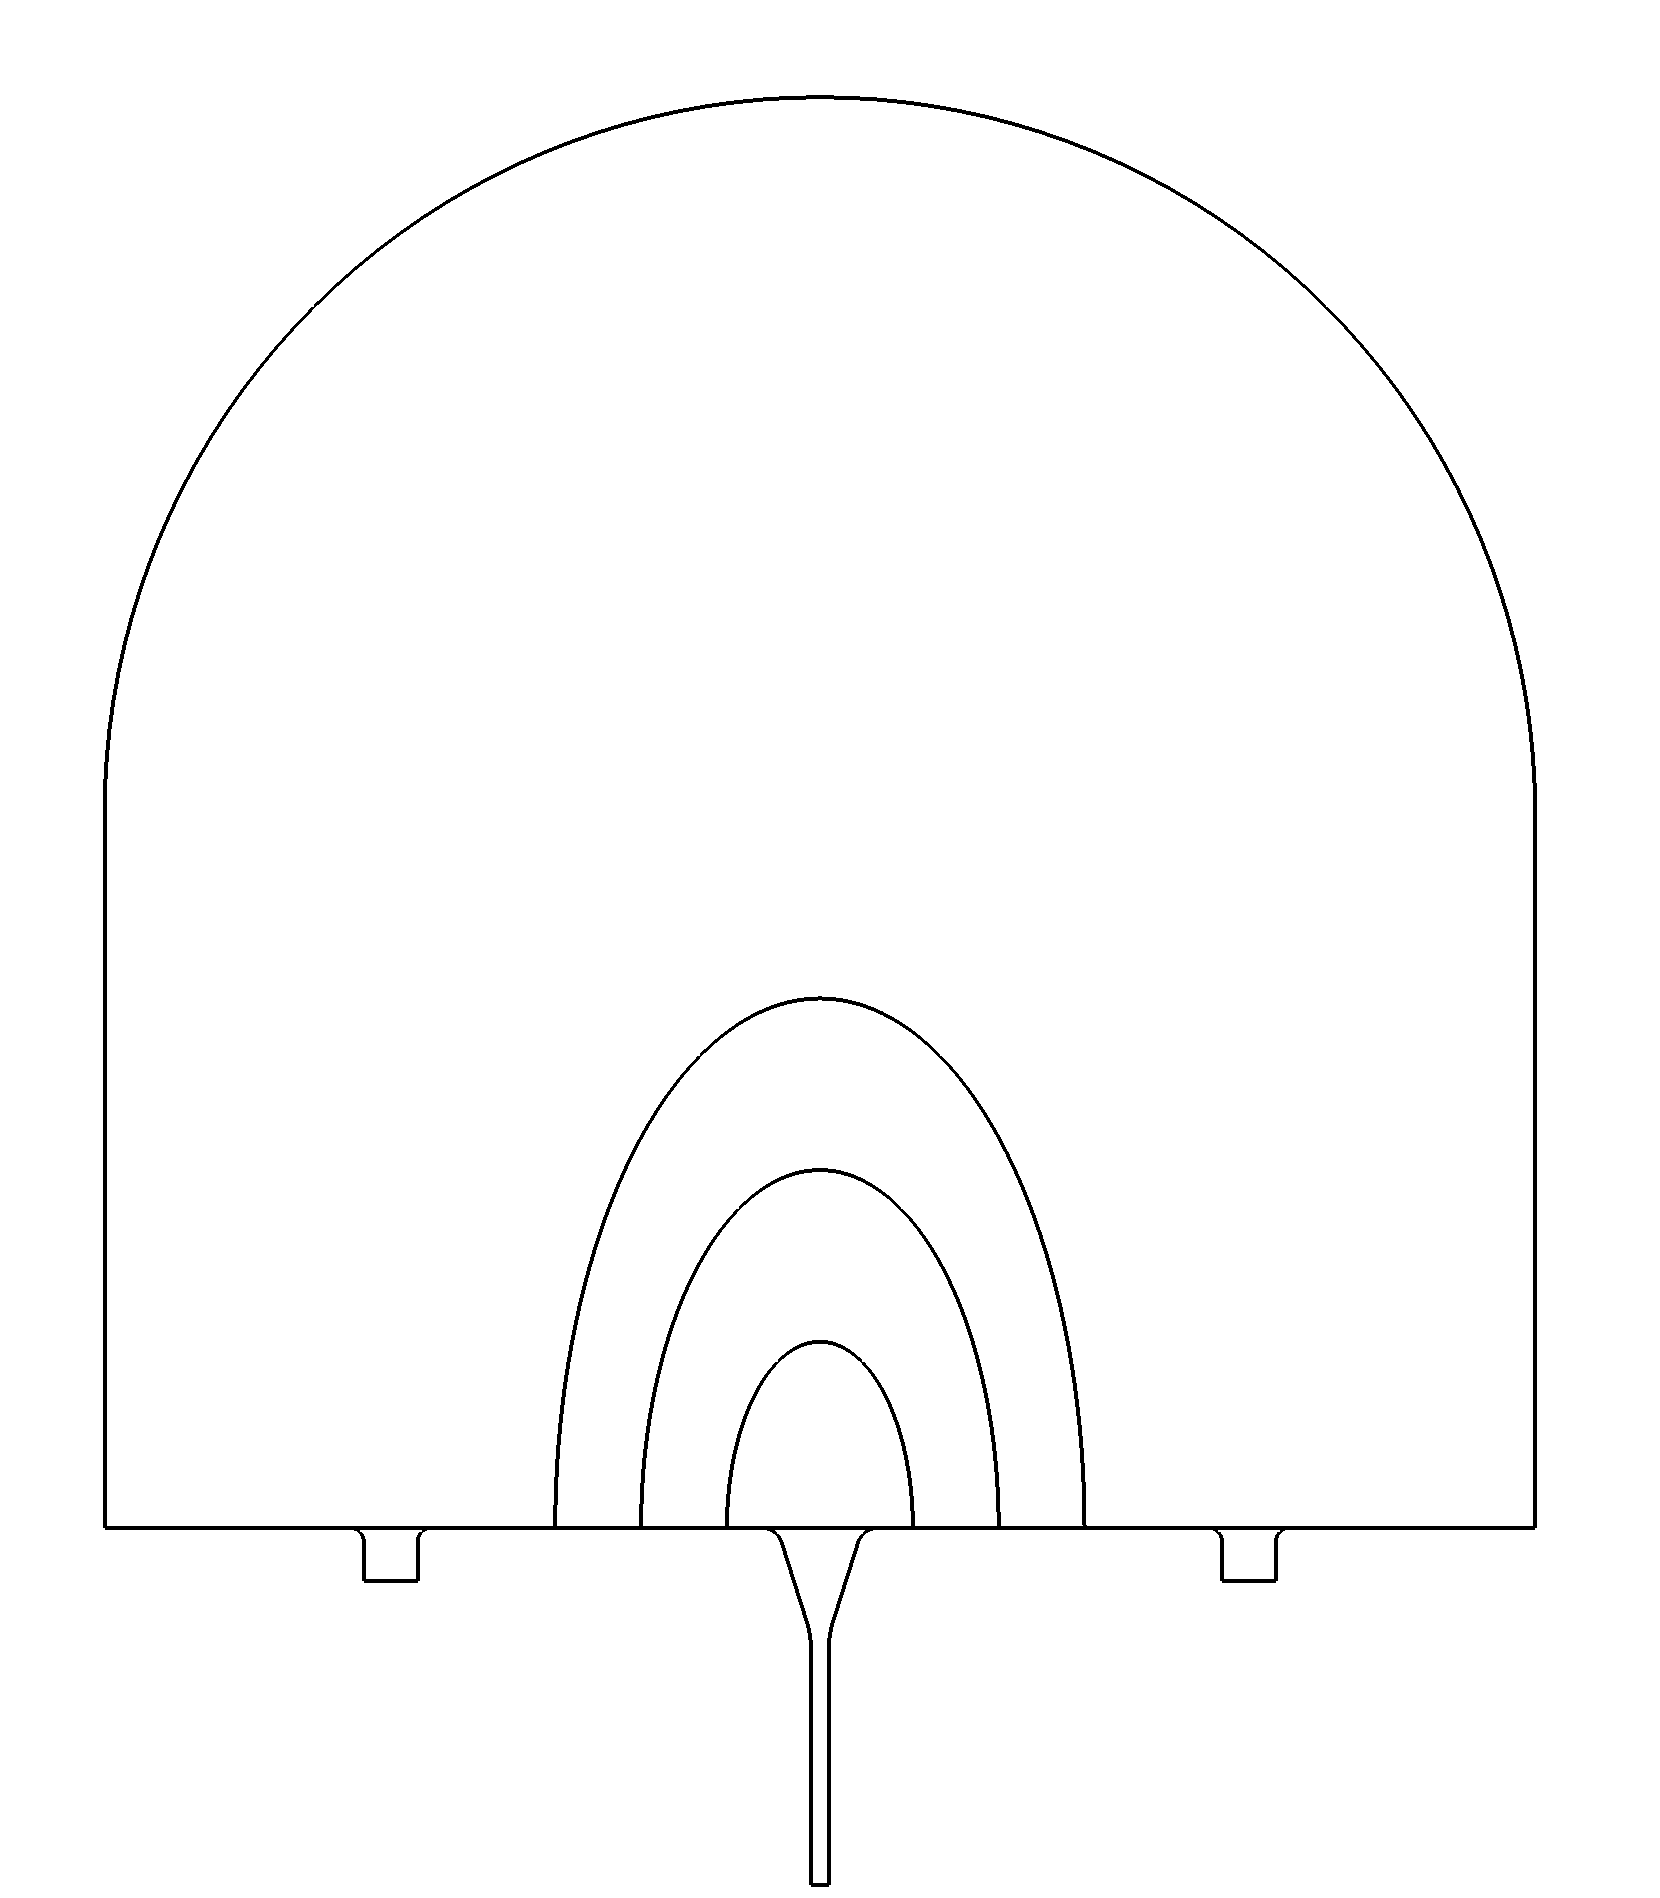
\includegraphics[width=189.6pt,height=216.78pt]{diagrams/placenta-geometry-diagrams/mesh_box-circle.png}};
%Shape: Axis 2D [id:dp020523494814431942] 
\draw  (146.18,293.48) -- (178.98,293.48)(149.46,263.96) -- (149.46,296.76) (171.98,288.48) -- (178.98,293.48) -- (171.98,298.48) (144.46,270.96) -- (149.46,263.96) -- (154.46,270.96)  ;

%Straight Lines [id:da8036713501202459] 
\draw [color={rgb, 255:red, 128; green, 128; blue, 128 }  ,draw opacity=1 ]   (429.5,304.49) -- (219,304.01) ;
\draw [shift={(216,304)}, rotate = 0.13] [fill={rgb, 255:red, 128; green, 128; blue, 128 }  ,fill opacity=1 ][line width=0.08]  [draw opacity=0] (7.14,-3.43) -- (0,0) -- (7.14,3.43) -- cycle    ;
\draw [shift={(432.5,304.5)}, rotate = 180.13] [fill={rgb, 255:red, 128; green, 128; blue, 128 }  ,fill opacity=1 ][line width=0.08]  [draw opacity=0] (7.14,-3.43) -- (0,0) -- (7.14,3.43) -- cycle    ;
%Straight Lines [id:da7908302902450595] 
\draw [color={rgb, 255:red, 155; green, 155; blue, 155 }  ,draw opacity=1 ] [dash pattern={on 0.84pt off 2.51pt}]  (432.5,246.5) -- (432.5,304.5) ;
%Straight Lines [id:da4155602358787114] 
\draw [color={rgb, 255:red, 155; green, 155; blue, 155 }  ,draw opacity=1 ] [dash pattern={on 0.84pt off 2.51pt}]  (216,246) -- (216,304) ;
%Shape: Rectangle [id:dp14174973381317724] 
\draw   (303.75,226.5) -- (343.5,226.5) -- (343.5,300.5) -- (303.75,300.5) -- cycle ;
%Shape: Polygon [id:ds3016551288537974] 
\draw  [fill={rgb, 255:red, 155; green, 155; blue, 155 }  ,fill opacity=0.2 ] (475.75,256.5) -- (343.5,300.5) -- (343.5,226.5) -- (475.75,57) -- cycle ;
%Shape: Rectangle [id:dp9578735364047417] 
\draw  [color={rgb, 255:red, 208; green, 2; blue, 27 }  ,draw opacity=1 ][fill={rgb, 255:red, 255; green, 255; blue, 255 }  ,fill opacity=1 ][line width=2.25] [blur shadow={shadow xshift=0pt,shadow yshift=0pt, shadow blur radius=1.5pt, shadow blur steps=4 ,shadow opacity=100}] (475.75,57) -- (647,57) -- (647,256.5) -- (475.75,256.5) -- cycle ;
%Shape: Rectangle [id:dp23171471463851145] 
\draw   (249.5,238.5) -- (269,238.5) -- (269,256.5) -- (249.5,256.5) -- cycle ;
%Shape: Polygon [id:ds957152197864789] 
\draw  [fill={rgb, 255:red, 155; green, 155; blue, 155 }  ,fill opacity=0.2 ] (249.5,238.5) -- (249.5,256.5) -- (174,154.5) -- (174,59) -- cycle ;
%Shape: Rectangle [id:dp5734000637247996] 
\draw  [color={rgb, 255:red, 74; green, 144; blue, 226 }  ,draw opacity=1 ][fill={rgb, 255:red, 255; green, 255; blue, 255 }  ,fill opacity=1 ][line width=2.25] [blur shadow={shadow xshift=0pt,shadow yshift=0pt, shadow blur radius=1.5pt, shadow blur steps=4 ,shadow opacity=100}] (23.5,59) -- (174,59) -- (174,154.5) -- (23.5,154.5) -- cycle ;
%Image [id:dp7627742527510089] 
\draw (542.33,151) node  {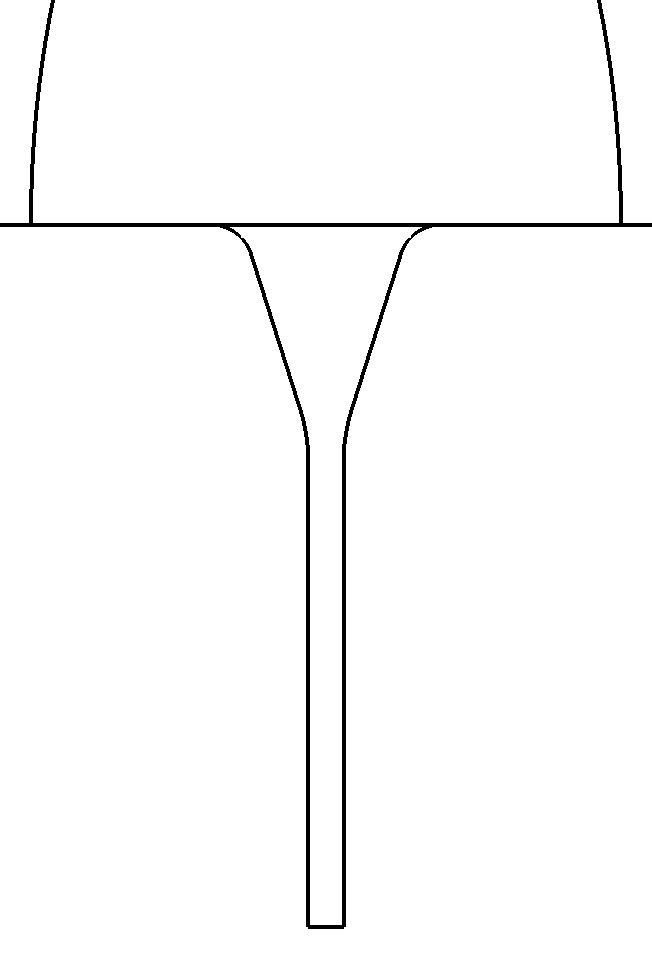
\includegraphics[width=81.5pt,height=121.5pt]{diagrams/placenta-geometry-diagrams/mesh_box-circle_artery.png}};
%Image [id:dp2920261793480039] 
\draw (92.04,105.25) node  {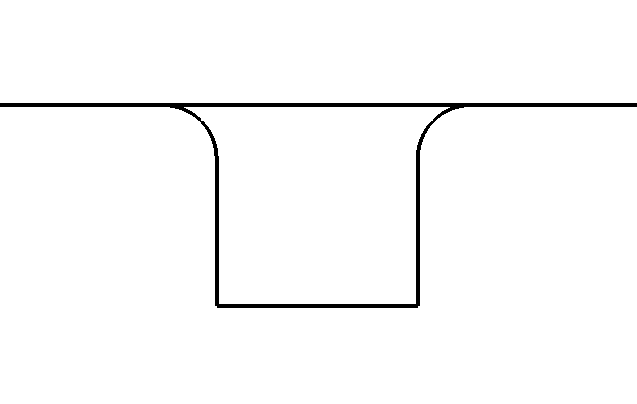
\includegraphics[width=97.56pt,height=61.88pt]{diagrams/placenta-geometry-diagrams/mesh_box-circle_vein.png}};
%Straight Lines [id:da007703491218846725] 
\draw [color={rgb, 255:red, 128; green, 128; blue, 128 }  ,draw opacity=1 ]   (109,130.75) -- (74.75,130.75) ;
\draw [shift={(71.75,130.75)}, rotate = 360] [fill={rgb, 255:red, 128; green, 128; blue, 128 }  ,fill opacity=1 ][line width=0.08]  [draw opacity=0] (5.36,-2.57) -- (0,0) -- (5.36,2.57) -- cycle    ;
\draw [shift={(112,130.75)}, rotate = 180] [fill={rgb, 255:red, 128; green, 128; blue, 128 }  ,fill opacity=1 ][line width=0.08]  [draw opacity=0] (5.36,-2.57) -- (0,0) -- (5.36,2.57) -- cycle    ;
%Straight Lines [id:da6675820105512444] 
\draw [color={rgb, 255:red, 128; green, 128; blue, 128 }  ,draw opacity=1 ]   (122,90.75) -- (122,123.25) ;
\draw [shift={(122,126.25)}, rotate = 270] [fill={rgb, 255:red, 128; green, 128; blue, 128 }  ,fill opacity=1 ][line width=0.08]  [draw opacity=0] (5.36,-2.57) -- (0,0) -- (5.36,2.57) -- cycle    ;
\draw [shift={(122,87.75)}, rotate = 90] [fill={rgb, 255:red, 128; green, 128; blue, 128 }  ,fill opacity=1 ][line width=0.08]  [draw opacity=0] (5.36,-2.57) -- (0,0) -- (5.36,2.57) -- cycle    ;
%Straight Lines [id:da020004946952280278] 
\draw [color={rgb, 255:red, 128; green, 128; blue, 128 }  ,draw opacity=1 ]   (555.5,103) -- (528.25,103) ;
\draw [shift={(525.25,103)}, rotate = 360] [fill={rgb, 255:red, 128; green, 128; blue, 128 }  ,fill opacity=1 ][line width=0.08]  [draw opacity=0] (5.36,-2.57) -- (0,0) -- (5.36,2.57) -- cycle    ;
\draw [shift={(558.5,103)}, rotate = 180] [fill={rgb, 255:red, 128; green, 128; blue, 128 }  ,fill opacity=1 ][line width=0.08]  [draw opacity=0] (5.36,-2.57) -- (0,0) -- (5.36,2.57) -- cycle    ;
%Straight Lines [id:da8088085573407642] 
\draw [color={rgb, 255:red, 155; green, 155; blue, 155 }  ,draw opacity=1 ] [dash pattern={on 0.84pt off 2.51pt}]  (546,144.5) -- (560.75,144.5) ;
%Straight Lines [id:da6668766321328388] 
\draw [color={rgb, 255:red, 155; green, 155; blue, 155 }  ,draw opacity=1 ] [dash pattern={on 0.84pt off 2.51pt}]  (546,224.25) -- (590.75,224.25) ;
%Straight Lines [id:da9239755653729449] 
\draw [color={rgb, 255:red, 128; green, 128; blue, 128 }  ,draw opacity=1 ]   (561.25,141.5) -- (561.25,111) ;
\draw [shift={(561.25,108)}, rotate = 90] [fill={rgb, 255:red, 128; green, 128; blue, 128 }  ,fill opacity=1 ][line width=0.08]  [draw opacity=0] (5.36,-2.57) -- (0,0) -- (5.36,2.57) -- cycle    ;
\draw [shift={(561.25,144.5)}, rotate = 270] [fill={rgb, 255:red, 128; green, 128; blue, 128 }  ,fill opacity=1 ][line width=0.08]  [draw opacity=0] (5.36,-2.57) -- (0,0) -- (5.36,2.57) -- cycle    ;
%Straight Lines [id:da9153150562330312] 
\draw [color={rgb, 255:red, 128; green, 128; blue, 128 }  ,draw opacity=1 ]   (590.75,221.25) -- (590.75,111.25) ;
\draw [shift={(590.75,108.25)}, rotate = 90] [fill={rgb, 255:red, 128; green, 128; blue, 128 }  ,fill opacity=1 ][line width=0.08]  [draw opacity=0] (7.14,-3.43) -- (0,0) -- (7.14,3.43) -- cycle    ;
\draw [shift={(590.75,224.25)}, rotate = 270] [fill={rgb, 255:red, 128; green, 128; blue, 128 }  ,fill opacity=1 ][line width=0.08]  [draw opacity=0] (7.14,-3.43) -- (0,0) -- (7.14,3.43) -- cycle    ;
%Straight Lines [id:da02336395841755401] 
\draw [color={rgb, 255:red, 128; green, 128; blue, 128 }  ,draw opacity=1 ]   (545.25,227.75) -- (539.5,227.75) ;
\draw [shift={(536.5,227.75)}, rotate = 360] [fill={rgb, 255:red, 128; green, 128; blue, 128 }  ,fill opacity=1 ][line width=0.08]  [draw opacity=0] (3.57,-1.72) -- (0,0) -- (3.57,1.72) -- cycle    ;
\draw [shift={(548.25,227.75)}, rotate = 180] [fill={rgb, 255:red, 128; green, 128; blue, 128 }  ,fill opacity=1 ][line width=0.08]  [draw opacity=0] (3.57,-1.72) -- (0,0) -- (3.57,1.72) -- cycle    ;

% Text Node
\draw (182.36,290) node [anchor=west] [inner sep=0.75pt]  [font=\footnotesize]  {$x$};
% Text Node
\draw (150.5,257.55) node [anchor=south] [inner sep=0.75pt]  [font=\footnotesize]  {$y$};
% Text Node
\draw (324.25,307.65) node [anchor=north] [inner sep=0.75pt]  [font=\footnotesize,color={rgb, 255:red, 128; green, 128; blue, 128 }  ,opacity=1 ]  {$40\ \text{mm}$};
% Text Node
\draw (91.88,134.15) node [anchor=north] [inner sep=0.75pt]  [font=\scriptsize,color={rgb, 255:red, 128; green, 128; blue, 128 }  ,opacity=1 ]  {$1.5\ \text{mm}$};
% Text Node
\draw (124,107) node [anchor=west] [inner sep=0.75pt]  [font=\scriptsize,color={rgb, 255:red, 128; green, 128; blue, 128 }  ,opacity=1 ]  {$1.5\ \text{mm}$};
% Text Node
\draw (541.88,99.6) node [anchor=south] [inner sep=0.75pt]  [font=\scriptsize,color={rgb, 255:red, 128; green, 128; blue, 128 }  ,opacity=1 ]  {$2.4\ \text{mm}$};
% Text Node
\draw (563.25,126.25) node [anchor=west] [inner sep=0.75pt]  [font=\tiny,color={rgb, 255:red, 128; green, 128; blue, 128 }  ,opacity=1 ]  {$3\ \text{mm}$};
% Text Node
\draw (592.75,166.25) node [anchor=west] [inner sep=0.75pt]  [font=\scriptsize,color={rgb, 255:red, 128; green, 128; blue, 128 }  ,opacity=1 ]  {$10\ \text{mm}$};
% Text Node
\draw (542.38,232.2) node [anchor=north] [inner sep=0.75pt]  [font=\tiny,color={rgb, 255:red, 128; green, 128; blue, 128 }  ,opacity=1 ]  {$0.5\ \text{mm}$};


\end{tikzpicture}

                    \caption{}
                    \label{fig:box-circle:dimensions}
                \end{subfigure}
                \begin{subfigure}{\textwidth}
                    \centering
                    

\tikzset{every picture/.style={line width=0.75pt}} %set default line width to 0.75pt        

\begin{tikzpicture}[x=0.75pt,y=0.75pt,yscale=-1,xscale=1]
%uncomment if require: \path (0,300); %set diagram left start at 0, and has height of 300

%Image [id:dp22126921700589142] 
\draw (324.42,148.98) node  {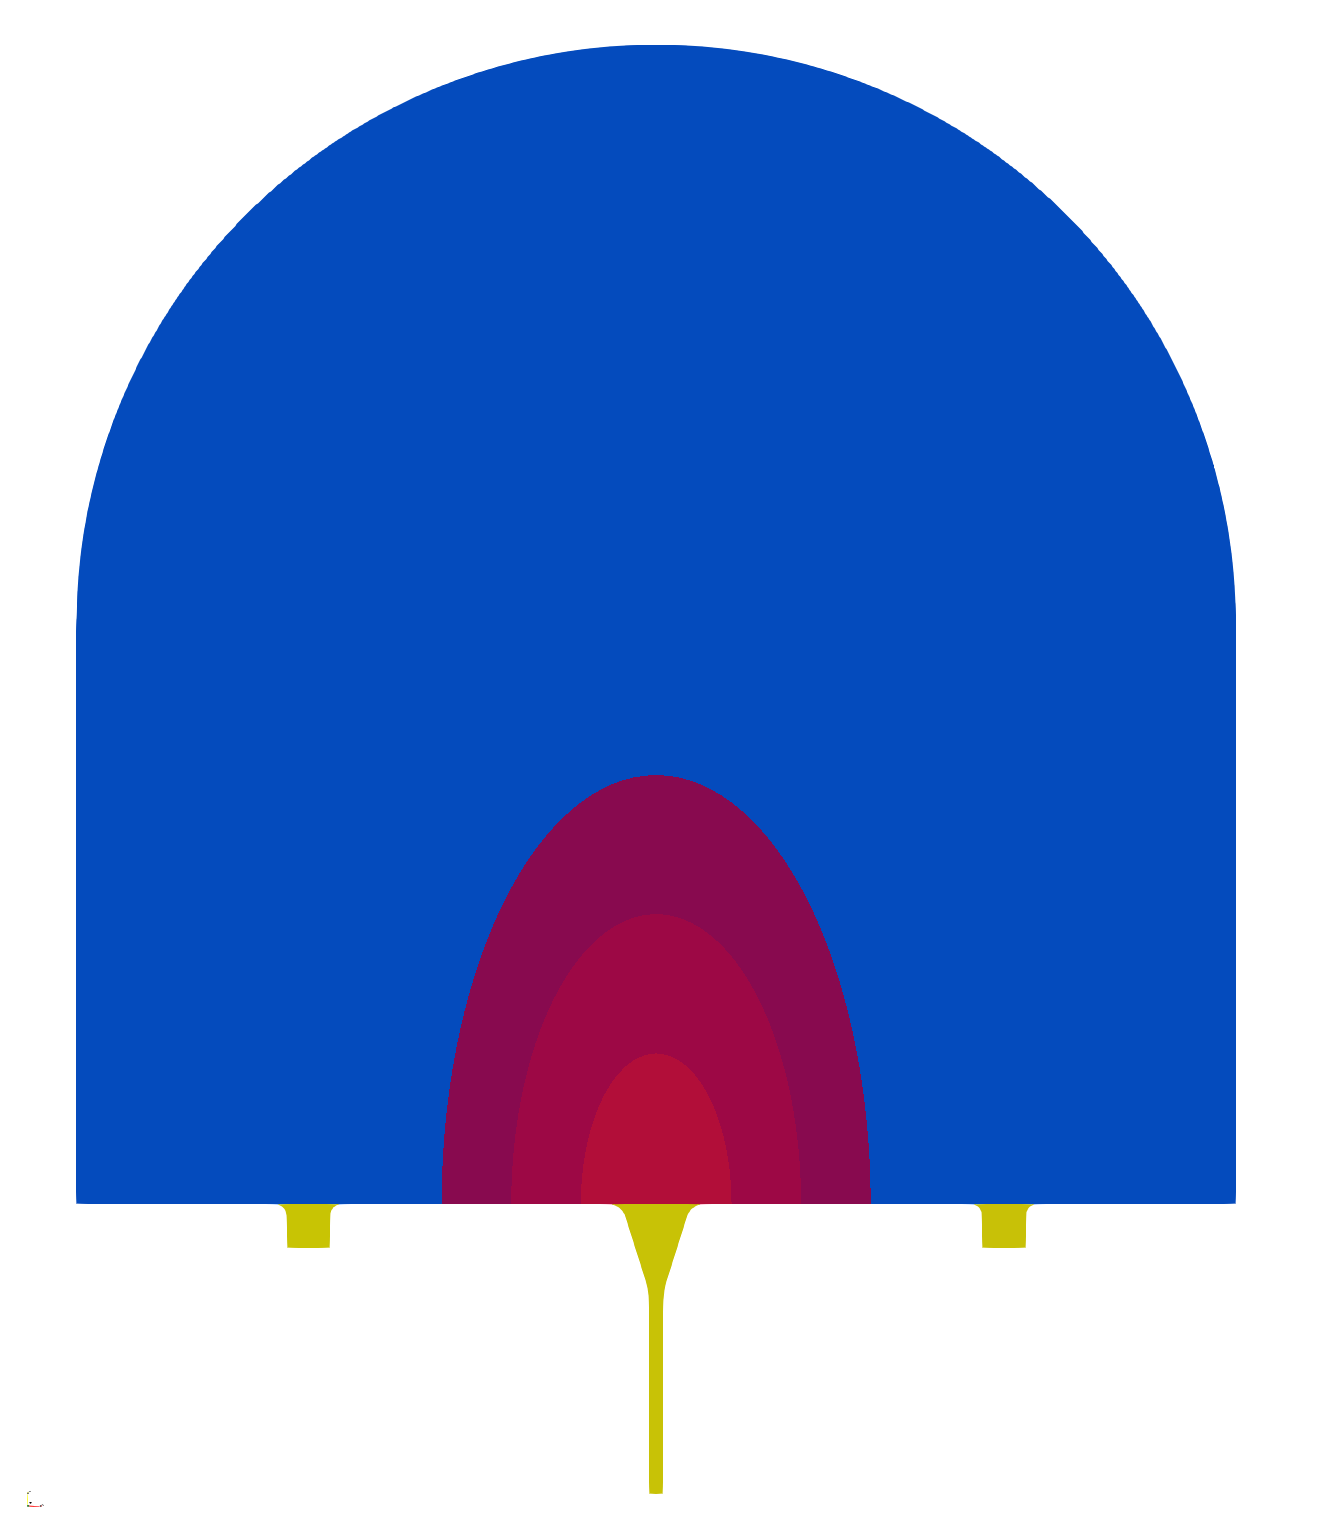
\includegraphics[width=190.54pt,height=218.28pt]{diagrams/placenta-geometry-diagrams/region_box-circle.png}};
%Shape: Rectangle [id:dp11952109232655417] 
\draw   (276.25,144.5) -- (368.5,144.5) -- (368.5,290) -- (276.25,290) -- cycle ;
%Shape: Polygon [id:ds32462111988530795] 
\draw  [fill={rgb, 255:red, 155; green, 155; blue, 155 }  ,fill opacity=0.2 ] (472.75,274.75) -- (368.5,290) -- (368.5,144.5) -- (472.75,47.5) -- cycle ;
%Shape: Rectangle [id:dp5451664654875743] 
\draw  [color={rgb, 255:red, 208; green, 2; blue, 27 }  ,draw opacity=1 ][fill={rgb, 255:red, 255; green, 255; blue, 255 }  ,fill opacity=1 ][line width=2.25] [blur shadow={shadow xshift=0pt,shadow yshift=0pt, shadow blur radius=1.5pt, shadow blur steps=4 ,shadow opacity=100}] (472.75,47.5) -- (628,47.5) -- (628,274.75) -- (472.75,274.75) -- cycle ;
%Shape: Rectangle [id:dp6890601408304888] 
\draw   (246.5,229) -- (266,229) -- (266,247) -- (246.5,247) -- cycle ;
%Shape: Polygon [id:ds42099539199351566] 
\draw  [fill={rgb, 255:red, 155; green, 155; blue, 155 }  ,fill opacity=0.2 ] (246.5,229) -- (246.5,247) -- (171,163.25) -- (171,49.5) -- cycle ;
%Shape: Rectangle [id:dp12209853757269817] 
\draw  [color={rgb, 255:red, 74; green, 144; blue, 226 }  ,draw opacity=1 ][fill={rgb, 255:red, 255; green, 255; blue, 255 }  ,fill opacity=1 ][line width=2.25] [blur shadow={shadow xshift=0pt,shadow yshift=0pt, shadow blur radius=1.5pt, shadow blur steps=4 ,shadow opacity=100}] (31,49.5) -- (171,49.5) -- (171,163.25) -- (31,163.25) -- cycle ;
%Shape: Axis 2D [id:dp5452843462335768] 
\draw  (143.68,262.48) -- (176.48,262.48)(146.96,232.96) -- (146.96,265.76) (169.48,257.48) -- (176.48,262.48) -- (169.48,267.48) (141.96,239.96) -- (146.96,232.96) -- (151.96,239.96)  ;

%Image [id:dp5542528854088136] 
\draw (550,147.64) node  {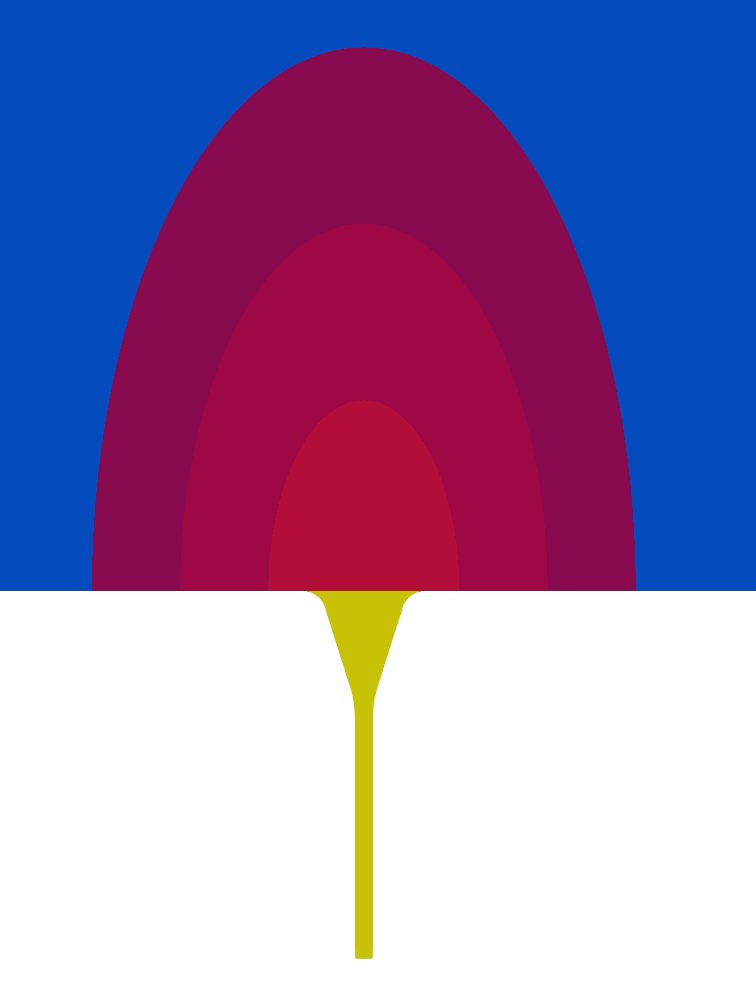
\includegraphics[width=107.25pt,height=141.58pt]{diagrams/placenta-geometry-diagrams/region_box-circle_artery.png}};
%Image [id:dp4703221885051676] 
\draw (101.5,97.38) node  {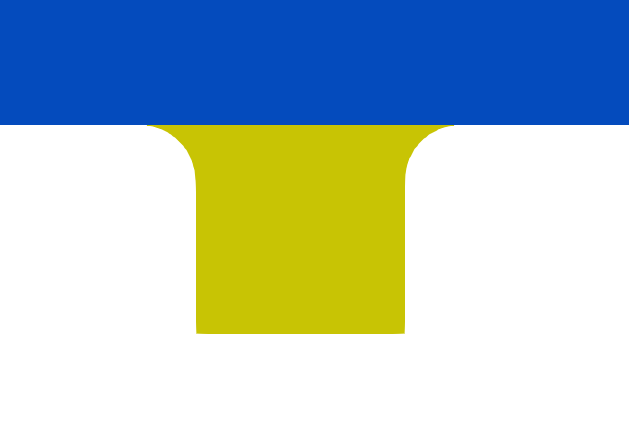
\includegraphics[width=96.75pt,height=65.06pt]{diagrams/placenta-geometry-diagrams/region_box-circle_vein.png}};
%Shape: Arc [id:dp15907837716166395] 
\draw  [draw opacity=0][line width=3.75]  (514.1,164.59) .. controls (514.1,164.5) and (514.1,164.42) .. (514.1,164.34) .. controls (514.1,126.41) and (529.36,95.67) .. (548.18,95.67) .. controls (567,95.67) and (582.25,126.41) .. (582.25,164.34) .. controls (582.25,164.46) and (582.25,164.59) .. (582.25,164.72) -- (548.18,164.34) -- cycle ; \draw  [line width=3.75]  (514.1,164.59) .. controls (514.1,164.5) and (514.1,164.42) .. (514.1,164.34) .. controls (514.1,126.41) and (529.36,95.67) .. (548.18,95.67) .. controls (567,95.67) and (582.25,126.41) .. (582.25,164.34) .. controls (582.25,164.46) and (582.25,164.59) .. (582.25,164.72) ;  
%Straight Lines [id:da31968378407565723] 
\draw    (523,204.5) -- (541.48,192.62) ;
\draw [shift={(544,191)}, rotate = 147.26] [fill={rgb, 255:red, 0; green, 0; blue, 0 }  ][line width=0.08]  [draw opacity=0] (8.93,-4.29) -- (0,0) -- (8.93,4.29) -- cycle    ;
%Straight Lines [id:da21169793883490962] 
\draw [color={rgb, 255:red, 74; green, 144; blue, 226 }  ,draw opacity=1 ][line width=3.75]    (120,122.25) -- (77.25,122.25) ;
%Straight Lines [id:da48410947011907224] 
\draw [color={rgb, 255:red, 208; green, 2; blue, 27 }  ,draw opacity=1 ][line width=2.25]    (549,233.5) -- (545.75,233.5) ;
%Straight Lines [id:da8968866603549419] 
\draw [color={rgb, 255:red, 178; green, 15; blue, 57 }  ,draw opacity=1 ]   (550.25,168.5) -- (595.5,168.5) ;
\draw [shift={(598.5,168.5)}, rotate = 180] [fill={rgb, 255:red, 178; green, 15; blue, 57 }  ,fill opacity=1 ][line width=0.08]  [draw opacity=0] (5.36,-2.57) -- (0,0) -- (5.36,2.57) -- cycle    ;
\draw [shift={(547.25,168.5)}, rotate = 0] [fill={rgb, 255:red, 178; green, 15; blue, 57 }  ,fill opacity=1 ][line width=0.08]  [draw opacity=0] (5.36,-2.57) -- (0,0) -- (5.36,2.57) -- cycle    ;
%Straight Lines [id:da31654998264540546] 
\draw [color={rgb, 255:red, 178; green, 15; blue, 57 }  ,draw opacity=1 ]   (550.5,176.5) -- (579.25,176.5) ;
\draw [shift={(582.25,176.5)}, rotate = 180] [fill={rgb, 255:red, 178; green, 15; blue, 57 }  ,fill opacity=1 ][line width=0.08]  [draw opacity=0] (5.36,-2.57) -- (0,0) -- (5.36,2.57) -- cycle    ;
\draw [shift={(547.5,176.5)}, rotate = 0] [fill={rgb, 255:red, 178; green, 15; blue, 57 }  ,fill opacity=1 ][line width=0.08]  [draw opacity=0] (5.36,-2.57) -- (0,0) -- (5.36,2.57) -- cycle    ;
%Straight Lines [id:da2804690215211083] 
\draw [color={rgb, 255:red, 178; green, 15; blue, 57 }  ,draw opacity=1 ]   (551.5,184.25) -- (562,184.25) ;
\draw [shift={(565,184.25)}, rotate = 180] [fill={rgb, 255:red, 178; green, 15; blue, 57 }  ,fill opacity=1 ][line width=0.08]  [draw opacity=0] (5.36,-2.57) -- (0,0) -- (5.36,2.57) -- cycle    ;
\draw [shift={(548.5,184.25)}, rotate = 0] [fill={rgb, 255:red, 178; green, 15; blue, 57 }  ,fill opacity=1 ][line width=0.08]  [draw opacity=0] (5.36,-2.57) -- (0,0) -- (5.36,2.57) -- cycle    ;
%Straight Lines [id:da2427007571257227] 
\draw [color={rgb, 255:red, 155; green, 155; blue, 155 }  ,draw opacity=1 ] [dash pattern={on 0.84pt off 2.51pt}]  (565,166) -- (565,184.25) ;
%Straight Lines [id:da6267655040295248] 
\draw [color={rgb, 255:red, 155; green, 155; blue, 155 }  ,draw opacity=1 ] [dash pattern={on 0.84pt off 2.51pt}]  (582.25,164.72) -- (582.25,176.75) ;
%Straight Lines [id:da38228961483549484] 
\draw [color={rgb, 255:red, 0; green, 0; blue, 0 }  ,draw opacity=1 ] [dash pattern={on 0.84pt off 2.51pt}]  (119,106.9) -- (77.67,106.9) ;
%Straight Lines [id:da182869504277962] 
\draw [color={rgb, 255:red, 178; green, 15; blue, 57 }  ,draw opacity=1 ]   (65.83,84.1) -- (65.83,102.67) ;
\draw [shift={(65.83,105.67)}, rotate = 270] [fill={rgb, 255:red, 178; green, 15; blue, 57 }  ,fill opacity=1 ][line width=0.08]  [draw opacity=0] (5.36,-2.57) -- (0,0) -- (5.36,2.57) -- cycle    ;
\draw [shift={(65.83,81.1)}, rotate = 90] [fill={rgb, 255:red, 178; green, 15; blue, 57 }  ,fill opacity=1 ][line width=0.08]  [draw opacity=0] (5.36,-2.57) -- (0,0) -- (5.36,2.57) -- cycle    ;
%Straight Lines [id:da6948815579213783] 
\draw [color={rgb, 255:red, 128; green, 128; blue, 128 }  ,draw opacity=1 ] [dash pattern={on 0.84pt off 2.51pt}]  (119.33,98.05) -- (77.45,98.05) ;
%Straight Lines [id:da547314772003725] 
\draw [color={rgb, 255:red, 128; green, 128; blue, 128 }  ,draw opacity=1 ] [dash pattern={on 0.84pt off 2.51pt}]  (119,88.47) -- (77.38,88.47) ;
%Straight Lines [id:da8083416036570497] 
\draw    (134.67,119.02) -- (124.92,116.69) ;
\draw [shift={(122,116)}, rotate = 13.39] [fill={rgb, 255:red, 0; green, 0; blue, 0 }  ][line width=0.08]  [draw opacity=0] (5.36,-2.57) -- (0,0) -- (5.36,2.57) -- cycle    ;

% Text Node
\draw (179.86,259) node [anchor=west] [inner sep=0.75pt]  [font=\footnotesize]  {$x$};
% Text Node
\draw (148,226.55) node [anchor=south] [inner sep=0.75pt]  [font=\footnotesize]  {$y$};
% Text Node
\draw (133.57,114.07) node [anchor=north west][inner sep=0.75pt]  [font=\Large,color={rgb, 255:red, 0; green, 0; blue, 0 }  ,opacity=1 ]  {$\Omega _{\text{v}}$};
% Text Node
\draw (101.21,65.91) node  [font=\normalsize,color={rgb, 255:red, 255; green, 255; blue, 255 }  ,opacity=1 ]  {$\Omega _{\text{IVS}}$};
% Text Node
\draw (547.79,150.91) node  [font=\small,color={rgb, 255:red, 255; green, 255; blue, 255 }  ,opacity=1 ]  {$\Omega _{\text{CC}}$};
% Text Node
\draw (598.79,69.25) node  [font=\large,color={rgb, 255:red, 255; green, 255; blue, 255 }  ,opacity=1 ]  {$\Omega _{\text{IVS}}$};
% Text Node
\draw (524.5,200.4) node [anchor=north east] [inner sep=0.75pt]  [font=\LARGE,color={rgb, 255:red, 0; green, 0; blue, 0 }  ,opacity=1 ]  {$\Omega _{\text{a}}$};
% Text Node
\draw (323.38,90.08) node  [font=\LARGE,color={rgb, 255:red, 255; green, 255; blue, 255 }  ,opacity=1 ]  {$\Omega _{\text{IVS}}$};
% Text Node
\draw (99.38,127.2) node [anchor=north] [inner sep=0.75pt]  [font=\Large,color={rgb, 255:red, 74; green, 144; blue, 226 }  ,opacity=1 ]  {$\Gamma _{\text{out}}$};
% Text Node
\draw (547.5,237.7) node [anchor=north] [inner sep=0.75pt]  [font=\Large,color={rgb, 255:red, 208; green, 2; blue, 27 }  ,opacity=1 ]  {$\Gamma _{\text{in}}$};
% Text Node
\draw (557.54,187.4) node [anchor=north] [inner sep=0.75pt]  [font=\small,color={rgb, 255:red, 178; green, 15; blue, 57 }  ,opacity=1 ]  {$s_{0}$};
% Text Node
\draw (574.29,179.65) node [anchor=north] [inner sep=0.75pt]  [font=\small,color={rgb, 255:red, 178; green, 15; blue, 57 }  ,opacity=1 ]  {$s_{1}$};
% Text Node
\draw (590.79,171.4) node [anchor=north] [inner sep=0.75pt]  [font=\small,color={rgb, 255:red, 178; green, 15; blue, 57 }  ,opacity=1 ]  {$s_{2}$};
% Text Node
\draw (550.29,118.41) node  [font=\small,color={rgb, 255:red, 255; green, 255; blue, 255 }  ,opacity=1 ]  {$\Omega {_{\text{T}^{-}}^{\ }}^{\ }$};
% Text Node
\draw (549.79,78.41) node  [font=\small,color={rgb, 255:red, 255; green, 255; blue, 255 }  ,opacity=1 ]  {$\Omega {_{\text{T}^{+}}^{\ }}^{\ }$};
% Text Node
\draw (62.07,92.59) node [anchor=east] [inner sep=0.75pt]  [font=\scriptsize,color={rgb, 255:red, 0; green, 0; blue, 0 }  ,opacity=1 ]  {$\textcolor[rgb]{0.64,0.04,0.26}{y}\textcolor[rgb]{0.64,0.04,0.26}{_{0}}$};


\end{tikzpicture}

                    \caption{}
                    \label{fig:box-circle:regions}
                \end{subfigure}
                \caption{Not to scale. Diagrams illustrating the 2D placentone geometry introduced in \S\ref{sec:modelling:geometries:2d-placentone}. (a) Diagram illustrating a simple 2D geometry for a single placentone with dimensions. The red box shows a zoomed-in view of the inlet location, and the blue box shows a zoomed-in view of one of the veins. (b) Diagram illustrating subdomains corresponding to $\Omega$ and its subdomains. The coloured boxes again show zoomed-in views with $\Gamma_\text{in}$ and $\Gamma_\text{out}$ indicated. Sizes of the cavity transition region are illustrated using $s_0$, $s_1$, and $s_2$, and sizes of the vein transition region are illustrated only for $y_0$ for ease of presentation; these sizes are used in Appendix \ref{sec:smooth-transition} to define $\Psi$.}
                \label{fig:box-circle}
            \end{figure}

        \subsection{2D placenta} \label{sec:modelling:geometries:2d-placenta}        
            A shortcoming of the single placentone model geometry described above is that flux of blood between neighbouring placentones is necessarily neglected, and additional drainage due to septal wall veins and marginal sinus veins have not been considered in flow models. We therefore present work on a physiologically representative 2D slice of a whole human placenta. This geometry consists of six adjacent placentones that are placed along an arc of a circle and is illustrated in \ref{fig:inverted-circle-slice-6-flat:dimensions}.

            To be precise, we assume a typical 3D placenta to be a spherical cap with a diameter of \qty{220}{\milli\meter} and maximum height of \qty{36.26}{\milli\meter}, containing $30$--$60$ placentones with widths decreasing toward the periphery \cite{benirschkePathologyHumanPlacenta2012,afrakhtehCorrelationPlacentalThickness2013,kaufmannPlacentalVascularizationBlood1988}. We therefore estimated that a 2D planar cross-section could contain approximately 6 placentones. We note that this assumes that this cross-section intersects perfectly through the centre of all inlets and outlets, and note that 6 placentones is possibly an under- or over-estimate of the true number found in a 2D slice; taking the image shown in Figure \ref{fig:placenta:lobules} as an example, we see that the numbers and sizes of placentones may vary greatly depending upon where the slice is taken; values from the literature also suggest that the number of placentones vary greatly from placenta-to-placenta \cite{benirschkePathologyHumanPlacenta2012,kaufmannPlacentalVascularizationBlood1988,serovOptimalVilliDensity2015}. We assume that there are impermeable walls (septal walls) of width \qty{3}{\milli\meter} and heights of either \qty{6.90}{\milli\meter} or \qty{14.07}{\milli\meter} between placentones \cite{AMANITIS2023e68}, with the two choices of height distinguishing between taller walls found between lobes and shorter walls found between lobules. We assume that all 6 placentones are located on an arc of a circle of centre $\vec{p} \equiv (p_1, p_2)^\intercal$, which is constructed such that the maximum height is \qty{36.26}{\milli\meter} \cite{afrakhtehCorrelationPlacentalThickness2013}; we note that the figures quoted here are to two decimal places, as they are averages over many samples. We have also added two corner outlets (called marginal sinuses) of widths \qtyproduct{3}{\milli\meter} in order to model additional drainage in each of the corners \cite{nanaevHumanPlacentaEncircled2000}. Following the work of several previous authors, we assume that placentones contain at most one artery and two veins on the basal plate of each placentone, where arteries diverge as they meet the central cavity \cite{chernyavskyMathematicalModelIntervillous2010,lecarpentierComputationalFluidDynamic2016,burtonRheologicalPhysiologicalConsequences2009}. We will also assume that septal walls contains at most 1 vein on the left side, top, and right side of each septal wall. Furthermore, we reduce the size of the placentones as they get closer to the periphery, with horizontal widths \qty{40}{\milli\meter}, \qty{33.85}{\milli\meter}, and \qty{28.65}{\milli\meter} from inner-most to outer-most placentones, forming a geometric progression. Central cavities are also added above arteries, which are normally-oriented to the basal plate, and decrease in size toward the periphery in proportion to the placentone widths. Each central cavity is created by an ellipse of semi-major axis \qty{10}{\milli\meter} and semi-minor axis \qty{5}{\milli\meter} that is tangential to a line passing directly through its spiral artery -- note that, unlike the 2D placentone, the cavity edges may not be normal where they meet the basal plate. We fillet the domain and split into non-overlapping subdomains, as done for the placentone geometry. These regions are illustrated in Figure \ref{fig:inverted-circle-slice-6-flat:regions}.

            We highlight that this 2D placenta geometry is a first-step towards modelling organ-scale maternal blood that respects larger structural features such as septal walls and marginal sinus veins. In contrast with previous studies on a placentone geometry, we allow the basal plate arteries, basal plate veins, and septal wall veins to be placed in any position along the basal plate, subject to a small number of constraints.

            This thesis will make use of the 2D placentone and placenta geometries in the following places. \S\ref{sec:numerical-methods:blood-flow-experiments:comparison} will initially make use of the placentone geometry with one artery and two veins, all of which remain in nominal positions along the basal plate. Next, \S\ref{sec:numerical-methods:blood-flow-experiments:asymmetric} will take the placenta geometry with one artery and \textit{one} vein per placentone, in order to create an asymmetric flow pattern. \S\ref{sec:nutrient-uptake:variation-of-vessels} will relax the assumption of the regular positioning and number of vessels, instead allowing any combination of vessels in any position. Chapters \ref{sec:numerical-mri} and \ref{sec:contractions} take the asymmetric placenta problem from \S\ref{sec:numerical-methods:blood-flow-experiments:asymmetric} to respectively compute MRI signals from simulated placental flow and compute flow on a contracting placenta.

            \begin{figure}
                \thisfloatpagestyle{empty}
                \begin{subfigure}[b]{\textwidth}
                    \centering
                    

\tikzset{every picture/.style={line width=0.75pt}} %set default line width to 0.75pt        

\begin{tikzpicture}[x=0.75pt,y=0.75pt,yscale=-1,xscale=1]
%uncomment if require: \path (0,398); %set diagram left start at 0, and has height of 398

%Image [id:dp80183306204371] 
\draw (331.09,278) node  {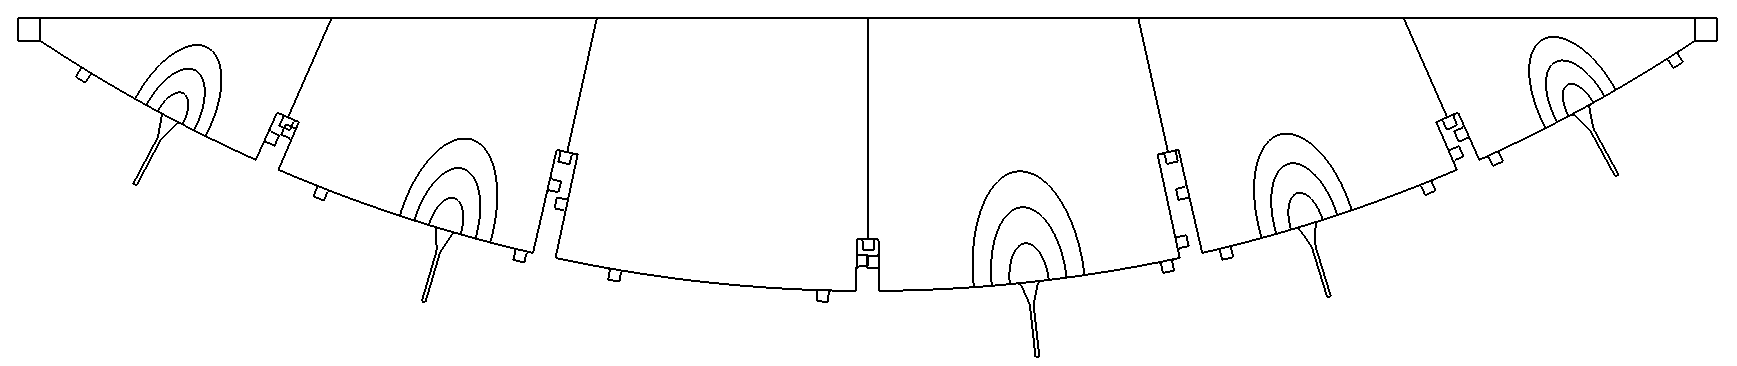
\includegraphics[width=473.38pt,height=100.5pt]{diagrams/placenta-geometry-diagrams/mesh_inverted-circle-slice-6-flat_normal-walls_septal-veins.png}};
%Shape: Polygon [id:ds599560967686122] 
\draw  [fill={rgb, 255:red, 155; green, 155; blue, 155 }  ,fill opacity=0.2 ] (436.42,180.33) -- (227,262.5) -- (215,262.5) -- (311.92,180.33) -- cycle ;
%Straight Lines [id:da3836552587833064] 
\draw [color={rgb, 255:red, 155; green, 155; blue, 155 }  ,draw opacity=1 ] [dash pattern={on 0.84pt off 2.51pt}]  (632.5,226.5) -- (632.5,345) ;
%Straight Lines [id:da8869549916108876] 
\draw [color={rgb, 255:red, 155; green, 155; blue, 155 }  ,draw opacity=1 ] [dash pattern={on 0.84pt off 2.51pt}]  (555,269) -- (555,345) ;
%Straight Lines [id:da08890647812691421] 
\draw [color={rgb, 255:red, 128; green, 128; blue, 128 }  ,draw opacity=1 ]   (558,345) -- (629.5,345) ;
\draw [shift={(632.5,345)}, rotate = 180] [fill={rgb, 255:red, 128; green, 128; blue, 128 }  ,fill opacity=1 ][line width=0.08]  [draw opacity=0] (7.14,-3.43) -- (0,0) -- (7.14,3.43) -- cycle    ;
\draw [shift={(555,345)}, rotate = 0] [fill={rgb, 255:red, 128; green, 128; blue, 128 }  ,fill opacity=1 ][line width=0.08]  [draw opacity=0] (7.14,-3.43) -- (0,0) -- (7.14,3.43) -- cycle    ;
%Straight Lines [id:da4569539433423251] 
\draw [color={rgb, 255:red, 155; green, 155; blue, 155 }  ,draw opacity=1 ] [dash pattern={on 0.84pt off 2.51pt}]  (545.5,273) -- (545.5,345) ;
%Straight Lines [id:da6425775020756577] 
\draw [color={rgb, 255:red, 155; green, 155; blue, 155 }  ,draw opacity=1 ] [dash pattern={on 0.84pt off 2.51pt}]  (453,303.5) -- (453,345) ;
%Straight Lines [id:da84971523704646] 
\draw [color={rgb, 255:red, 155; green, 155; blue, 155 }  ,draw opacity=1 ] [dash pattern={on 0.84pt off 2.51pt}]  (445.5,303.5) -- (445.5,344) ;
%Straight Lines [id:da4522901839526503] 
\draw [color={rgb, 255:red, 155; green, 155; blue, 155 }  ,draw opacity=1 ] [dash pattern={on 0.84pt off 2.51pt}]  (334.5,316) -- (334.5,344) ;
%Straight Lines [id:da886100326010987] 
\draw [color={rgb, 255:red, 128; green, 128; blue, 128 }  ,draw opacity=1 ]   (337.5,345) -- (442,345) ;
\draw [shift={(445,345)}, rotate = 180] [fill={rgb, 255:red, 128; green, 128; blue, 128 }  ,fill opacity=1 ][line width=0.08]  [draw opacity=0] (7.14,-3.43) -- (0,0) -- (7.14,3.43) -- cycle    ;
\draw [shift={(334.5,345)}, rotate = 0] [fill={rgb, 255:red, 128; green, 128; blue, 128 }  ,fill opacity=1 ][line width=0.08]  [draw opacity=0] (7.14,-3.43) -- (0,0) -- (7.14,3.43) -- cycle    ;
%Straight Lines [id:da2739622055496771] 
\draw [color={rgb, 255:red, 155; green, 155; blue, 155 }  ,draw opacity=1 ] [dash pattern={on 0.84pt off 2.51pt}]  (28.5,226.5) -- (28.5,345) ;
%Straight Lines [id:da8223757430798608] 
\draw [color={rgb, 255:red, 155; green, 155; blue, 155 }  ,draw opacity=1 ] [dash pattern={on 0.84pt off 2.51pt}]  (105.87,269.5) -- (105.87,345) ;
%Straight Lines [id:da9585020997428355] 
\draw [color={rgb, 255:red, 128; green, 128; blue, 128 }  ,draw opacity=1 ]   (102.87,345) -- (31.5,345) ;
\draw [shift={(28.5,345)}, rotate = 360] [fill={rgb, 255:red, 128; green, 128; blue, 128 }  ,fill opacity=1 ][line width=0.08]  [draw opacity=0] (7.14,-3.43) -- (0,0) -- (7.14,3.43) -- cycle    ;
\draw [shift={(105.87,345)}, rotate = 180] [fill={rgb, 255:red, 128; green, 128; blue, 128 }  ,fill opacity=1 ][line width=0.08]  [draw opacity=0] (7.14,-3.43) -- (0,0) -- (7.14,3.43) -- cycle    ;
%Straight Lines [id:da7396996741803523] 
\draw [color={rgb, 255:red, 155; green, 155; blue, 155 }  ,draw opacity=1 ] [dash pattern={on 0.84pt off 2.51pt}]  (115.35,273) -- (115.35,345) ;
%Straight Lines [id:da7690060794723255] 
\draw [color={rgb, 255:red, 155; green, 155; blue, 155 }  ,draw opacity=1 ] [dash pattern={on 0.84pt off 2.51pt}]  (207.7,303) -- (207.7,345) ;
%Straight Lines [id:da1750801006916194] 
\draw [color={rgb, 255:red, 155; green, 155; blue, 155 }  ,draw opacity=1 ] [dash pattern={on 0.84pt off 2.51pt}]  (215.19,305) -- (215.19,344) ;
%Straight Lines [id:da36519166335869224] 
\draw [color={rgb, 255:red, 155; green, 155; blue, 155 }  ,draw opacity=1 ] [dash pattern={on 0.84pt off 2.51pt}]  (326,316.5) -- (326,344) ;
%Straight Lines [id:da5227117484890365] 
\draw [color={rgb, 255:red, 128; green, 128; blue, 128 }  ,draw opacity=1 ]   (323,345) -- (218.69,345) ;
\draw [shift={(215.69,345)}, rotate = 360] [fill={rgb, 255:red, 128; green, 128; blue, 128 }  ,fill opacity=1 ][line width=0.08]  [draw opacity=0] (7.14,-3.43) -- (0,0) -- (7.14,3.43) -- cycle    ;
\draw [shift={(326,345)}, rotate = 180] [fill={rgb, 255:red, 128; green, 128; blue, 128 }  ,fill opacity=1 ][line width=0.08]  [draw opacity=0] (7.14,-3.43) -- (0,0) -- (7.14,3.43) -- cycle    ;
%Straight Lines [id:da9869684148666715] 
\draw [color={rgb, 255:red, 128; green, 128; blue, 128 }  ,draw opacity=1 ]   (204.2,345) -- (118.35,345) ;
\draw [shift={(115.35,345)}, rotate = 360] [fill={rgb, 255:red, 128; green, 128; blue, 128 }  ,fill opacity=1 ][line width=0.08]  [draw opacity=0] (7.14,-3.43) -- (0,0) -- (7.14,3.43) -- cycle    ;
\draw [shift={(207.2,345)}, rotate = 180] [fill={rgb, 255:red, 128; green, 128; blue, 128 }  ,fill opacity=1 ][line width=0.08]  [draw opacity=0] (7.14,-3.43) -- (0,0) -- (7.14,3.43) -- cycle    ;
%Shape: Rectangle [id:dp7784307888916284] 
\draw   (379,303.5) -- (396.5,303.5) -- (396.5,341.5) -- (379,341.5) -- cycle ;
%Shape: Rectangle [id:dp7413532166529391] 
\draw   (18,215.27) -- (35.5,215.27) -- (35.5,228.77) -- (18,228.77) -- cycle ;
%Shape: Rectangle [id:dp1083356594712217] 
\draw   (305.17,310.67) -- (322.67,310.67) -- (322.67,326.17) -- (305.17,326.17) -- cycle ;
%Shape: Polygon [id:ds13903772067200593] 
\draw  [fill={rgb, 255:red, 155; green, 155; blue, 155 }  ,fill opacity=0.2 ] (635,183) -- (396.5,303.5) -- (379,303.5) -- (463.75,183) -- cycle ;
%Shape: Polygon [id:ds6960752336656928] 
\draw  [fill={rgb, 255:red, 155; green, 155; blue, 155 }  ,fill opacity=0.2 ] (139.25,187.75) -- (35.5,215.27) -- (18,215.27) -- (14.75,187.75) -- cycle ;
%Shape: Polygon [id:ds16525050807756858] 
\draw  [fill={rgb, 255:red, 155; green, 155; blue, 155 }  ,fill opacity=0.2 ] (436.42,180.33) -- (322.67,310.67) -- (305.17,310.67) -- (311.92,180.33) -- cycle ;
%Shape: Rectangle [id:dp6070840373099016] 
\draw  [color={rgb, 255:red, 208; green, 2; blue, 27 }  ,draw opacity=1 ][fill={rgb, 255:red, 255; green, 255; blue, 255 }  ,fill opacity=1 ][line width=2.25] [blur shadow={shadow xshift=0pt,shadow yshift=0pt, shadow blur radius=1.5pt, shadow blur steps=4 ,shadow opacity=100}] (463.75,22.5) -- (635,22.5) -- (635,183) -- (463.75,183) -- cycle ;
%Image [id:dp7341682961381069] 
\draw (523.25,97.77) node  {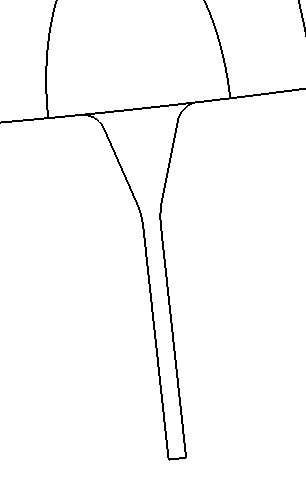
\includegraphics[width=54.75pt,height=89.28pt]{diagrams/placenta-geometry-diagrams/mesh_inverted-circle-slice-6-flat_normal-walls-septal-veins_artery.png}};
%Straight Lines [id:da2560686325124286] 
\draw [color={rgb, 255:red, 155; green, 155; blue, 155 }  ,draw opacity=1 ] [dash pattern={on 0.84pt off 2.51pt}]  (532.75,63) -- (575,57.75) ;
%Straight Lines [id:da862538474933769] 
\draw [color={rgb, 255:red, 155; green, 155; blue, 155 }  ,draw opacity=1 ] [dash pattern={on 0.84pt off 2.51pt}]  (531.25,150.75) -- (585.75,143.5) ;
%Straight Lines [id:da07631904575656989] 
\draw [color={rgb, 255:red, 128; green, 128; blue, 128 }  ,draw opacity=1 ]   (585.36,137.02) -- (575.64,61.98) ;
\draw [shift={(575.25,59)}, rotate = 82.61] [fill={rgb, 255:red, 128; green, 128; blue, 128 }  ,fill opacity=1 ][line width=0.08]  [draw opacity=0] (7.14,-3.43) -- (0,0) -- (7.14,3.43) -- cycle    ;
\draw [shift={(585.75,140)}, rotate = 262.61] [fill={rgb, 255:red, 128; green, 128; blue, 128 }  ,fill opacity=1 ][line width=0.08]  [draw opacity=0] (7.14,-3.43) -- (0,0) -- (7.14,3.43) -- cycle    ;
%Straight Lines [id:da9334742103638392] 
\draw [color={rgb, 255:red, 128; green, 128; blue, 128 }  ,draw opacity=1 ]   (526.19,150.18) -- (492.5,129.5) ;
\draw [shift={(528.75,151.75)}, rotate = 211.54] [fill={rgb, 255:red, 128; green, 128; blue, 128 }  ,fill opacity=1 ][line width=0.08]  [draw opacity=0] (6.25,-3) -- (0,0) -- (6.25,3) -- cycle    ;
%Straight Lines [id:da644000948100526] 
\draw [color={rgb, 255:red, 128; green, 128; blue, 128 }  ,draw opacity=1 ]   (535.18,86.02) -- (533.07,65.98) ;
\draw [shift={(532.75,63)}, rotate = 83.96] [fill={rgb, 255:red, 128; green, 128; blue, 128 }  ,fill opacity=1 ][line width=0.08]  [draw opacity=0] (5.36,-2.57) -- (0,0) -- (5.36,2.57) -- cycle    ;
\draw [shift={(535.5,89)}, rotate = 263.96] [fill={rgb, 255:red, 128; green, 128; blue, 128 }  ,fill opacity=1 ][line width=0.08]  [draw opacity=0] (5.36,-2.57) -- (0,0) -- (5.36,2.57) -- cycle    ;
%Straight Lines [id:da058958443439840025] 
\draw [color={rgb, 255:red, 155; green, 155; blue, 155 }  ,draw opacity=1 ] [dash pattern={on 0.84pt off 2.51pt}]  (526,89.75) -- (535.5,89) ;
%Straight Lines [id:da635774139796158] 
\draw [color={rgb, 255:red, 128; green, 128; blue, 128 }  ,draw opacity=1 ]   (528.02,57.33) -- (509.23,59.42) ;
\draw [shift={(506.25,59.75)}, rotate = 353.66] [fill={rgb, 255:red, 128; green, 128; blue, 128 }  ,fill opacity=1 ][line width=0.08]  [draw opacity=0] (5.36,-2.57) -- (0,0) -- (5.36,2.57) -- cycle    ;
\draw [shift={(531,57)}, rotate = 173.66] [fill={rgb, 255:red, 128; green, 128; blue, 128 }  ,fill opacity=1 ][line width=0.08]  [draw opacity=0] (5.36,-2.57) -- (0,0) -- (5.36,2.57) -- cycle    ;
%Shape: Rectangle [id:dp12087627646558885] 
\draw  [color={rgb, 255:red, 74; green, 144; blue, 226 }  ,draw opacity=1 ][fill={rgb, 255:red, 255; green, 255; blue, 255 }  ,fill opacity=1 ][line width=2.25] [blur shadow={shadow xshift=0pt,shadow yshift=0pt, shadow blur radius=1.5pt, shadow blur steps=4 ,shadow opacity=100}] (311.92,51.5) -- (436.42,51.5) -- (436.42,180.33) -- (311.92,180.33) -- cycle ;
%Image [id:dp11084122971065935] 
\draw (362.92,87.84) node  {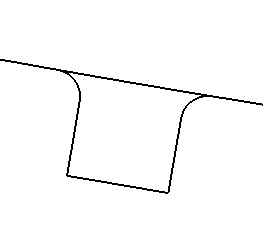
\includegraphics[width=56.25pt,height=51.76pt]{diagrams/placenta-geometry-diagrams/mesh_inverted-circle-slice-6-flat_normal-walls-septal-veins_vein.png}};
%Straight Lines [id:da4260411781736031] 
\draw [color={rgb, 255:red, 128; green, 128; blue, 128 }  ,draw opacity=1 ]   (371.2,114.18) -- (344.25,110.16) ;
\draw [shift={(341.28,109.72)}, rotate = 8.49] [fill={rgb, 255:red, 128; green, 128; blue, 128 }  ,fill opacity=1 ][line width=0.08]  [draw opacity=0] (5.36,-2.57) -- (0,0) -- (5.36,2.57) -- cycle    ;
\draw [shift={(374.17,114.63)}, rotate = 188.49] [fill={rgb, 255:red, 128; green, 128; blue, 128 }  ,fill opacity=1 ][line width=0.08]  [draw opacity=0] (5.36,-2.57) -- (0,0) -- (5.36,2.57) -- cycle    ;
%Straight Lines [id:da13622705064859697] 
\draw [color={rgb, 255:red, 128; green, 128; blue, 128 }  ,draw opacity=1 ]   (383.91,85.29) -- (380.42,105.63) ;
\draw [shift={(379.92,108.58)}, rotate = 279.73] [fill={rgb, 255:red, 128; green, 128; blue, 128 }  ,fill opacity=1 ][line width=0.08]  [draw opacity=0] (5.36,-2.57) -- (0,0) -- (5.36,2.57) -- cycle    ;
\draw [shift={(384.42,82.33)}, rotate = 99.73] [fill={rgb, 255:red, 128; green, 128; blue, 128 }  ,fill opacity=1 ][line width=0.08]  [draw opacity=0] (5.36,-2.57) -- (0,0) -- (5.36,2.57) -- cycle    ;
%Shape: Rectangle [id:dp043044360722185315] 
\draw  [color={rgb, 255:red, 74; green, 144; blue, 226 }  ,draw opacity=1 ][fill={rgb, 255:red, 255; green, 255; blue, 255 }  ,fill opacity=1 ][line width=2.25] [blur shadow={shadow xshift=0pt,shadow yshift=0pt, shadow blur radius=1.5pt, shadow blur steps=4 ,shadow opacity=100}] (14.75,110.5) -- (139.25,110.5) -- (139.25,187.75) -- (14.75,187.75) -- cycle ;
%Image [id:dp43909768466905374] 
\draw (88.25,149.86) node [xscale=-1] {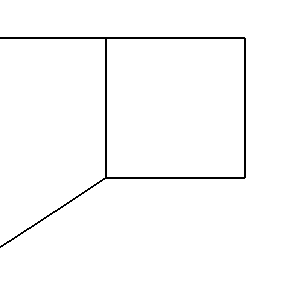
\includegraphics[width=52.5pt,height=53.05pt]{diagrams/placenta-geometry-diagrams/mesh_inverted-circle-slice-6-flat_normal-walls-septal-veins_marginal-sinus.png}};
%Straight Lines [id:da33088686310200743] 
\draw [color={rgb, 255:red, 128; green, 128; blue, 128 }  ,draw opacity=1 ]   (94,161.75) -- (66.75,161.75) ;
\draw [shift={(63.75,161.75)}, rotate = 360] [fill={rgb, 255:red, 128; green, 128; blue, 128 }  ,fill opacity=1 ][line width=0.08]  [draw opacity=0] (5.36,-2.57) -- (0,0) -- (5.36,2.57) -- cycle    ;
\draw [shift={(97,161.75)}, rotate = 180] [fill={rgb, 255:red, 128; green, 128; blue, 128 }  ,fill opacity=1 ][line width=0.08]  [draw opacity=0] (5.36,-2.57) -- (0,0) -- (5.36,2.57) -- cycle    ;
%Straight Lines [id:da3164833140775334] 
\draw [color={rgb, 255:red, 128; green, 128; blue, 128 }  ,draw opacity=1 ]   (57.75,125.5) -- (57.75,152.75) ;
\draw [shift={(57.75,155.75)}, rotate = 270] [fill={rgb, 255:red, 128; green, 128; blue, 128 }  ,fill opacity=1 ][line width=0.08]  [draw opacity=0] (5.36,-2.57) -- (0,0) -- (5.36,2.57) -- cycle    ;
\draw [shift={(57.75,122.5)}, rotate = 90] [fill={rgb, 255:red, 128; green, 128; blue, 128 }  ,fill opacity=1 ][line width=0.08]  [draw opacity=0] (5.36,-2.57) -- (0,0) -- (5.36,2.57) -- cycle    ;
%Shape: Rectangle [id:dp3214087399382912] 
\draw  [color={rgb, 255:red, 65; green, 117; blue, 5 }  ,draw opacity=1 ][dash pattern={on 2.53pt off 3.02pt}][line width=2.25]  (264.5,303) -- (281.5,303) -- (281.5,320) -- (264.5,320) -- cycle ;
%Shape: Axis 2D [id:dp5493960903283415] 
\draw  (10.68,368.48) -- (43.48,368.48)(13.96,338.96) -- (13.96,371.76) (36.48,363.48) -- (43.48,368.48) -- (36.48,373.48) (8.96,345.96) -- (13.96,338.96) -- (18.96,345.96)  ;

%Straight Lines [id:da8673543563072263] 
\draw [color={rgb, 255:red, 65; green, 117; blue, 5 }  ,draw opacity=1 ]   (244.5,173) -- (273.01,293.58) ;
\draw [shift={(273.7,296.5)}, rotate = 256.7] [fill={rgb, 255:red, 65; green, 117; blue, 5 }  ,fill opacity=1 ][line width=0.08]  [draw opacity=0] (8.93,-4.29) -- (0,0) -- (8.93,4.29) -- cycle    ;
%Straight Lines [id:da15777572686334396] 
\draw [color={rgb, 255:red, 128; green, 128; blue, 128 }  ,draw opacity=1 ]   (456.5,345) -- (542.5,345) ;
\draw [shift={(545.5,345)}, rotate = 180] [fill={rgb, 255:red, 128; green, 128; blue, 128 }  ,fill opacity=1 ][line width=0.08]  [draw opacity=0] (7.14,-3.43) -- (0,0) -- (7.14,3.43) -- cycle    ;
\draw [shift={(453.5,345)}, rotate = 0] [fill={rgb, 255:red, 128; green, 128; blue, 128 }  ,fill opacity=1 ][line width=0.08]  [draw opacity=0] (7.14,-3.43) -- (0,0) -- (7.14,3.43) -- cycle    ;
%Straight Lines [id:da20967786638483576] 
\draw [color={rgb, 255:red, 128; green, 128; blue, 128 }  ,draw opacity=1 ]   (126.53,260.24) -- (121.97,270.51) ;
\draw [shift={(120.75,273.25)}, rotate = 293.96] [fill={rgb, 255:red, 128; green, 128; blue, 128 }  ,fill opacity=1 ][line width=0.08]  [draw opacity=0] (3.57,-1.72) -- (0,0) -- (3.57,1.72) -- cycle    ;
\draw [shift={(127.75,257.5)}, rotate = 113.96] [fill={rgb, 255:red, 128; green, 128; blue, 128 }  ,fill opacity=1 ][line width=0.08]  [draw opacity=0] (3.57,-1.72) -- (0,0) -- (3.57,1.72) -- cycle    ;
%Straight Lines [id:da999991789814658] 
\draw [color={rgb, 255:red, 128; green, 128; blue, 128 }  ,draw opacity=1 ]   (228.14,272.19) -- (222.1,301.15) ;
\draw [shift={(221.49,304.09)}, rotate = 281.77] [fill={rgb, 255:red, 128; green, 128; blue, 128 }  ,fill opacity=1 ][line width=0.08]  [draw opacity=0] (3.57,-1.72) -- (0,0) -- (3.57,1.72) -- cycle    ;
\draw [shift={(228.75,269.25)}, rotate = 101.77] [fill={rgb, 255:red, 128; green, 128; blue, 128 }  ,fill opacity=1 ][line width=0.08]  [draw opacity=0] (3.57,-1.72) -- (0,0) -- (3.57,1.72) -- cycle    ;
%Shape: Rectangle [id:dp842610769802747] 
\draw   (215,262.5) -- (227,262.5) -- (227,272.5) -- (215,272.5) -- cycle ;
%Shape: Rectangle [id:dp34481258515956204] 
\draw  [color={rgb, 255:red, 65; green, 117; blue, 5 }  ,draw opacity=1 ][dash pattern={on 2.53pt off 3.02pt}][line width=2.25]  (94,260.5) -- (106,260.5) -- (106,272) -- (94,272) -- cycle ;
%Straight Lines [id:da484653672836302] 
\draw [color={rgb, 255:red, 65; green, 117; blue, 5 }  ,draw opacity=1 ]   (187.5,196.5) -- (107.93,254.24) ;
\draw [shift={(105.5,256)}, rotate = 324.03] [fill={rgb, 255:red, 65; green, 117; blue, 5 }  ,fill opacity=1 ][line width=0.08]  [draw opacity=0] (8.93,-4.29) -- (0,0) -- (8.93,4.29) -- cycle    ;

% Text Node
\draw (67.18,348.4) node [anchor=north] [inner sep=0.75pt]  [font=\footnotesize,color={rgb, 255:red, 128; green, 128; blue, 128 }  ,opacity=1 ]  {$28.65\ \text{mm}$};
% Text Node
\draw (161.28,348.4) node [anchor=north] [inner sep=0.75pt]  [font=\footnotesize,color={rgb, 255:red, 128; green, 128; blue, 128 }  ,opacity=1 ]  {$33.85\ \text{mm}$};
% Text Node
\draw (270.84,348.4) node [anchor=north] [inner sep=0.75pt]  [font=\footnotesize,color={rgb, 255:red, 128; green, 128; blue, 128 }  ,opacity=1 ]  {$40\ \text{mm}$};
% Text Node
\draw (389.75,348.4) node [anchor=north] [inner sep=0.75pt]  [font=\footnotesize,color={rgb, 255:red, 128; green, 128; blue, 128 }  ,opacity=1 ]  {$40\ \text{mm}$};
% Text Node
\draw (499.5,348.4) node [anchor=north] [inner sep=0.75pt]  [font=\footnotesize,color={rgb, 255:red, 128; green, 128; blue, 128 }  ,opacity=1 ]  {$33.85\ \text{mm}$};
% Text Node
\draw (593.75,348.4) node [anchor=north] [inner sep=0.75pt]  [font=\footnotesize,color={rgb, 255:red, 128; green, 128; blue, 128 }  ,opacity=1 ]  {$28.65\ \text{mm}$};
% Text Node
\draw (582.5,99.5) node [anchor=west] [inner sep=0.75pt]  [font=\footnotesize,color={rgb, 255:red, 128; green, 128; blue, 128 }  ,opacity=1 ]  {$10\ \text{mm}$};
% Text Node
\draw (512.64,126.72) node [anchor=south east] [inner sep=0.75pt]  [font=\scriptsize,color={rgb, 255:red, 128; green, 128; blue, 128 }  ,opacity=1 ]  {$0.5\ \text{mm}$};
% Text Node
\draw (536.13,76) node [anchor=west] [inner sep=0.75pt]  [font=\scriptsize,color={rgb, 255:red, 128; green, 128; blue, 128 }  ,opacity=1 ]  {$3\ \text{mm}$};
% Text Node
\draw (518.63,54.98) node [anchor=south] [inner sep=0.75pt]  [font=\scriptsize,color={rgb, 255:red, 128; green, 128; blue, 128 }  ,opacity=1 ]  {$2.4\ \text{mm}$};
% Text Node
\draw (80.38,165.15) node [anchor=north] [inner sep=0.75pt]  [font=\scriptsize,color={rgb, 255:red, 128; green, 128; blue, 128 }  ,opacity=1 ]  {$3\ \text{mm}$};
% Text Node
\draw (55.75,139.13) node [anchor=east] [inner sep=0.75pt]  [font=\scriptsize,color={rgb, 255:red, 128; green, 128; blue, 128 }  ,opacity=1 ]  {$3\ \text{mm}$};
% Text Node
\draw (357.22,115.53) node [anchor=north] [inner sep=0.75pt]  [font=\scriptsize,color={rgb, 255:red, 128; green, 128; blue, 128 }  ,opacity=1 ,rotate=-8.49]  {$1.5\ \text{mm}$};
% Text Node
\draw (384.14,95.75) node [anchor=west] [inner sep=0.75pt]  [font=\scriptsize,color={rgb, 255:red, 128; green, 128; blue, 128 }  ,opacity=1 ,rotate=-8.49]  {$1.5\ \text{mm}$};
% Text Node
\draw (46.86,365) node [anchor=west] [inner sep=0.75pt]  [font=\footnotesize]  {$x$};
% Text Node
\draw (15,332.55) node [anchor=south] [inner sep=0.75pt]  [font=\footnotesize]  {$y$};
% Text Node
\draw (373.4,139.41) node [anchor=north] [inner sep=0.75pt]  [font=\small] [align=left] {\textcolor[rgb]{0.29,0.56,0.89}{basal plate and}\\\textcolor[rgb]{0.29,0.56,0.89}{septal wall veins}};
% Text Node
\draw (545.5,174.4) node [anchor=south] [inner sep=0.75pt]  [font=\small,color={rgb, 255:red, 208; green, 2; blue, 27 }  ,opacity=1 ] [align=left] {spiral artery};
% Text Node
\draw (126.02,266.74) node [anchor=west] [inner sep=0.75pt]  [font=\tiny,color={rgb, 255:red, 128; green, 128; blue, 128 }  ,opacity=1 ,rotate=-23.4]  {$6.90\ \text{mm}$};
% Text Node
\draw (227.07,287.11) node [anchor=west] [inner sep=0.75pt]  [font=\tiny,color={rgb, 255:red, 128; green, 128; blue, 128 }  ,opacity=1 ,rotate=-12.55]  {$14.07\ \text{mm}$};
% Text Node
\draw (202.23,156.01) node [anchor=north west][inner sep=0.75pt]  [font=\small,color={rgb, 255:red, 65; green, 117; blue, 5 }  ,opacity=1 ] [align=left] {omitted artery};
% Text Node
\draw (153.73,179.51) node [anchor=north west][inner sep=0.75pt]  [font=\small,color={rgb, 255:red, 65; green, 117; blue, 5 }  ,opacity=1 ] [align=left] {omitted vein};


\end{tikzpicture}

                    \caption{}
                    \label{fig:inverted-circle-slice-6-flat:dimensions}
                \end{subfigure}
                \begin{subfigure}[b]{\textwidth}
                    \centering
                    

\tikzset{every picture/.style={line width=0.75pt}} %set default line width to 0.75pt        

\begin{tikzpicture}[x=0.75pt,y=0.75pt,yscale=-1,xscale=1]
%uncomment if require: \path (0,287); %set diagram left start at 0, and has height of 287

%Image [id:dp6789989035032795] 
\draw (331.45,190.67) node  {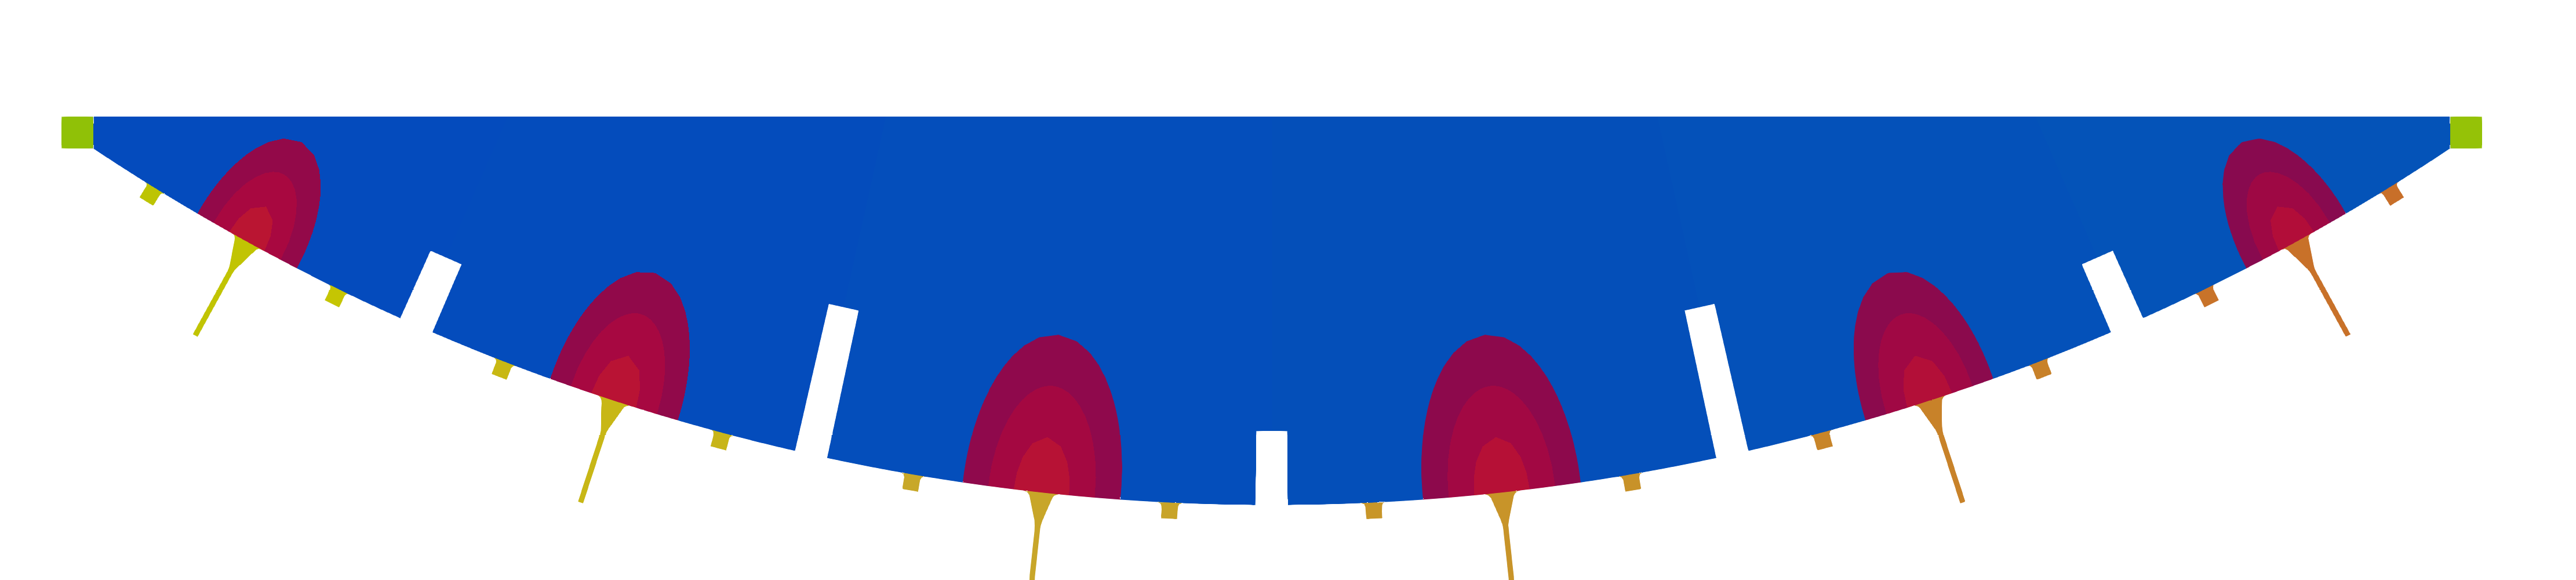
\includegraphics[width=482.17pt,height=108.5pt]{diagrams/placenta-geometry-diagrams/region_inverted-circle-slice-6-flat_normal-walls.png}};
%Shape: Polygon [id:ds5403154356225157] 
\draw  [fill={rgb, 255:red, 155; green, 155; blue, 155 }  ,fill opacity=0.2 ] (472.82,276.51) -- (410.33,270) -- (410.33,197.67) -- (472.82,13.58) -- cycle ;
%Shape: Rectangle [id:dp4374039436651571] 
\draw   (359.25,197.67) -- (410.33,197.67) -- (410.33,270) -- (359.25,270) -- cycle ;
%Shape: Rectangle [id:dp8847560919034154] 
\draw   (19.67,140.67) -- (37.17,140.67) -- (37.17,158.42) -- (19.67,158.42) -- cycle ;
%Shape: Rectangle [id:dp5761346961280844] 
\draw   (230.08,231.83) -- (247.58,231.83) -- (247.58,247.33) -- (230.08,247.33) -- cycle ;
%Shape: Polygon [id:ds6386627939021934] 
\draw  [fill={rgb, 255:red, 155; green, 155; blue, 155 }  ,fill opacity=0.2 ] (171.58,112.75) -- (37.17,140.67) -- (19.67,140.67) -- (15.25,112.75) -- cycle ;
%Shape: Polygon [id:ds9675166776770578] 
\draw  [fill={rgb, 255:red, 155; green, 155; blue, 155 }  ,fill opacity=0.2 ] (384.08,130) -- (247.58,231.83) -- (230.08,231.83) -- (259.58,130) -- cycle ;
%Shape: Rectangle [id:dp40877732662413346] 
\draw  [color={rgb, 255:red, 74; green, 144; blue, 226 }  ,draw opacity=1 ][fill={rgb, 255:red, 255; green, 255; blue, 255 }  ,fill opacity=1 ][line width=2.25] [blur shadow={shadow xshift=0pt,shadow yshift=0pt, shadow blur radius=1.5pt, shadow blur steps=4 ,shadow opacity=100}] (259.58,27.8) -- (384.08,27.8) -- (384.08,130) -- (259.58,130) -- cycle ;
%Shape: Rectangle [id:dp3581407575862343] 
\draw  [color={rgb, 255:red, 74; green, 144; blue, 226 }  ,draw opacity=1 ][fill={rgb, 255:red, 255; green, 255; blue, 255 }  ,fill opacity=1 ][line width=2.25] [blur shadow={shadow xshift=0pt,shadow yshift=0pt, shadow blur radius=1.5pt, shadow blur steps=4 ,shadow opacity=100}] (15.25,19.67) -- (171.58,19.67) -- (171.58,112.75) -- (15.25,112.75) -- cycle ;
%Image [id:dp5821978380209227] 
\draw (106.1,65.26) node  {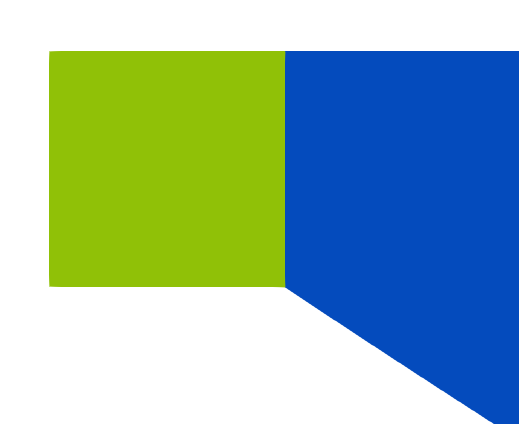
\includegraphics[width=75.15pt,height=61.39pt]{diagrams/placenta-geometry-diagrams/region_inverted-circle-slice-6-flat_normal-walls_marginal-sinus.png}};
%Straight Lines [id:da3775297991043933] 
\draw [color={rgb, 255:red, 74; green, 144; blue, 226 }  ,draw opacity=1 ][line width=3.75]    (330.25,101.5) -- (302,97.25) ;
%Straight Lines [id:da9001565707068373] 
\draw [color={rgb, 255:red, 74; green, 144; blue, 226 }  ,draw opacity=1 ][line width=3.75]    (65.25,79.75) -- (65.25,34.25) ;
%Shape: Axis 2D [id:dp5537933186782882] 
\draw  (10.68,267.79) -- (43.48,267.79)(13.96,238.27) -- (13.96,271.07) (36.48,262.79) -- (43.48,267.79) -- (36.48,272.79) (8.96,245.27) -- (13.96,238.27) -- (18.96,245.27)  ;

%Shape: Rectangle [id:dp6146437218873158] 
\draw  [color={rgb, 255:red, 208; green, 2; blue, 27 }  ,draw opacity=1 ][fill={rgb, 255:red, 255; green, 255; blue, 255 }  ,fill opacity=1 ][line width=2.25] [blur shadow={shadow xshift=0pt,shadow yshift=0pt, shadow blur radius=1.5pt, shadow blur steps=4 ,shadow opacity=100}] (472.82,13.58) -- (645.15,13.58) -- (645.15,276.51) -- (472.82,276.51) -- cycle ;
%Image [id:dp8106950500710235] 
\draw (560.93,139.16) node  {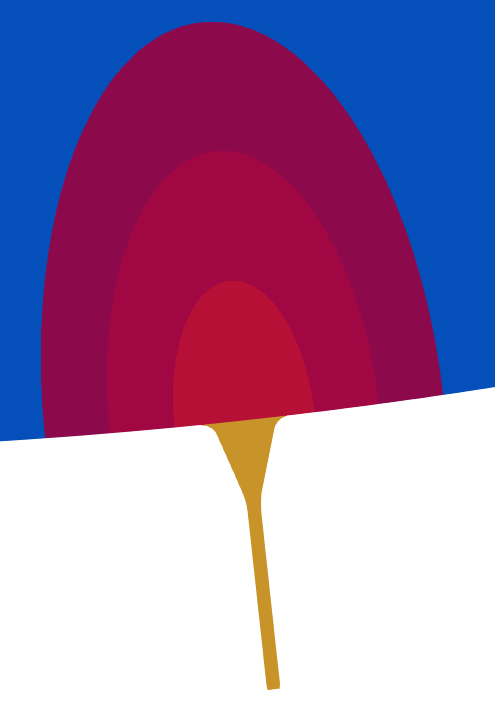
\includegraphics[width=117.17pt,height=171.38pt]{diagrams/placenta-geometry-diagrams/region_inverted-circle-slice-6-flat_normal-walls_artery.png}};
%Shape: Arc [id:dp897401775896993] 
\draw  [draw opacity=0][line width=3.75]  (518.97,160.96) .. controls (518.96,160.86) and (518.95,160.76) .. (518.94,160.66) .. controls (514.6,115.21) and (529.36,76.62) .. (551.91,74.46) .. controls (574.31,72.32) and (595.97,106.92) .. (600.53,151.92) -- (559.78,156.76) -- cycle ; \draw  [line width=3.75]  (518.97,160.96) .. controls (518.96,160.86) and (518.95,160.76) .. (518.94,160.66) .. controls (514.6,115.21) and (529.36,76.62) .. (551.91,74.46) .. controls (574.31,72.32) and (595.97,106.92) .. (600.53,151.92) ;  
%Straight Lines [id:da8094844692675482] 
\draw    (526.82,210.91) -- (556.86,194.36) ;
\draw [shift={(559.48,192.91)}, rotate = 151.14] [fill={rgb, 255:red, 0; green, 0; blue, 0 }  ][line width=0.08]  [draw opacity=0] (8.93,-4.29) -- (0,0) -- (8.93,4.29) -- cycle    ;
%Straight Lines [id:da3729402376326847] 
\draw [color={rgb, 255:red, 208; green, 2; blue, 27 }  ,draw opacity=1 ][line width=2.25]    (571.15,241.16) -- (567.15,241.66) ;
%Straight Lines [id:da14537836403413262] 
\draw [color={rgb, 255:red, 155; green, 155; blue, 155 }  ,draw opacity=1 ] [dash pattern={on 0.84pt off 2.51pt}]  (583.37,175.64) -- (581.15,154.91) ;
%Straight Lines [id:da6003461463769395] 
\draw [color={rgb, 255:red, 155; green, 155; blue, 155 }  ,draw opacity=1 ] [dash pattern={on 0.84pt off 2.51pt}]  (602.13,164.6) -- (600.53,151.92) ;
%Image [id:dp29326967503664414] 
\draw (320.41,80.83) node  {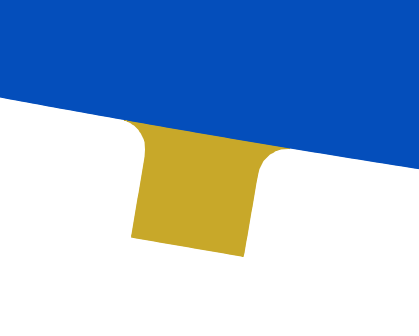
\includegraphics[width=79.62pt,height=63.85pt]{diagrams/placenta-geometry-diagrams/region_inverted-circle-slice-6-flat_normal-walls_vein.png}};
%Straight Lines [id:da9436862634001915] 
\draw [color={rgb, 255:red, 178; green, 15; blue, 57 }  ,draw opacity=1 ]   (566.73,177.64) -- (580.39,176) ;
\draw [shift={(583.37,175.64)}, rotate = 173.14] [fill={rgb, 255:red, 178; green, 15; blue, 57 }  ,fill opacity=1 ][line width=0.08]  [draw opacity=0] (5.36,-2.57) -- (0,0) -- (5.36,2.57) -- cycle    ;
\draw [shift={(563.75,178)}, rotate = 353.14] [fill={rgb, 255:red, 178; green, 15; blue, 57 }  ,fill opacity=1 ][line width=0.08]  [draw opacity=0] (5.36,-2.57) -- (0,0) -- (5.36,2.57) -- cycle    ;
%Straight Lines [id:da9114914997274575] 
\draw [color={rgb, 255:red, 178; green, 15; blue, 57 }  ,draw opacity=1 ]   (564.98,169.14) -- (599.15,164.96) ;
\draw [shift={(602.13,164.6)}, rotate = 173.03] [fill={rgb, 255:red, 178; green, 15; blue, 57 }  ,fill opacity=1 ][line width=0.08]  [draw opacity=0] (5.36,-2.57) -- (0,0) -- (5.36,2.57) -- cycle    ;
\draw [shift={(562,169.5)}, rotate = 353.03] [fill={rgb, 255:red, 178; green, 15; blue, 57 }  ,fill opacity=1 ][line width=0.08]  [draw opacity=0] (5.36,-2.57) -- (0,0) -- (5.36,2.57) -- cycle    ;
%Straight Lines [id:da8852053594450542] 
\draw [color={rgb, 255:red, 178; green, 15; blue, 57 }  ,draw opacity=1 ]   (564.48,160.39) -- (619.02,153.86) ;
\draw [shift={(622,153.5)}, rotate = 173.17] [fill={rgb, 255:red, 178; green, 15; blue, 57 }  ,fill opacity=1 ][line width=0.08]  [draw opacity=0] (5.36,-2.57) -- (0,0) -- (5.36,2.57) -- cycle    ;
\draw [shift={(561.5,160.75)}, rotate = 353.17] [fill={rgb, 255:red, 178; green, 15; blue, 57 }  ,fill opacity=1 ][line width=0.08]  [draw opacity=0] (5.36,-2.57) -- (0,0) -- (5.36,2.57) -- cycle    ;
%Straight Lines [id:da9553990232091423] 
\draw [color={rgb, 255:red, 74; green, 144; blue, 226 }  ,draw opacity=1 ][line width=3.75]    (329.25,103) -- (300.5,97.5) ;
%Straight Lines [id:da9713029290513338] 
\draw    (353.4,105.62) -- (336.4,95.9) ;
\draw [shift={(333.8,94.42)}, rotate = 29.74] [fill={rgb, 255:red, 0; green, 0; blue, 0 }  ][line width=0.08]  [draw opacity=0] (7.14,-3.43) -- (0,0) -- (7.14,3.43) -- cycle    ;
%Straight Lines [id:da5454083808690029] 
\draw [color={rgb, 255:red, 0; green, 0; blue, 0 }  ,draw opacity=1 ] [dash pattern={on 0.84pt off 2.51pt}]  (339.25,89.52) -- (303.5,82.27) ;
%Straight Lines [id:da8936020822292747] 
\draw [color={rgb, 255:red, 178; green, 15; blue, 57 }  ,draw opacity=1 ]   (341.4,78.94) -- (339.85,86.58) ;
\draw [shift={(339.25,89.52)}, rotate = 281.5] [fill={rgb, 255:red, 178; green, 15; blue, 57 }  ,fill opacity=1 ][line width=0.08]  [draw opacity=0] (3.57,-1.72) -- (0,0) -- (3.57,1.72) -- cycle    ;
\draw [shift={(342,76)}, rotate = 101.5] [fill={rgb, 255:red, 178; green, 15; blue, 57 }  ,fill opacity=1 ][line width=0.08]  [draw opacity=0] (3.57,-1.72) -- (0,0) -- (3.57,1.72) -- cycle    ;
%Straight Lines [id:da49992139569120564] 
\draw [color={rgb, 255:red, 0; green, 0; blue, 0 }  ,draw opacity=1 ] [dash pattern={on 0.84pt off 2.51pt}]  (91.6,77.97) -- (91.91,44.01) -- (92,33.57) ;
%Straight Lines [id:da35794129578966505] 
\draw    (55,93.02) -- (71.76,82.51) ;
\draw [shift={(74.3,80.92)}, rotate = 147.91] [fill={rgb, 255:red, 0; green, 0; blue, 0 }  ][line width=0.08]  [draw opacity=0] (7.14,-3.43) -- (0,0) -- (7.14,3.43) -- cycle    ;
%Straight Lines [id:da44499881038098454] 
\draw [color={rgb, 255:red, 178; green, 15; blue, 57 }  ,draw opacity=1 ]   (94.5,82.8) -- (108,82.98) ;
\draw [shift={(111,83.02)}, rotate = 180.73] [fill={rgb, 255:red, 178; green, 15; blue, 57 }  ,fill opacity=1 ][line width=0.08]  [draw opacity=0] (5.36,-2.57) -- (0,0) -- (5.36,2.57) -- cycle    ;
\draw [shift={(91.5,82.77)}, rotate = 0.73] [fill={rgb, 255:red, 178; green, 15; blue, 57 }  ,fill opacity=1 ][line width=0.08]  [draw opacity=0] (5.36,-2.57) -- (0,0) -- (5.36,2.57) -- cycle    ;
%Straight Lines [id:da602787461013311] 
\draw [color={rgb, 255:red, 128; green, 128; blue, 128 }  ,draw opacity=1 ] [dash pattern={on 0.84pt off 2.51pt}]  (98.15,77.87) -- (98.55,33.47) ;
%Straight Lines [id:da9481149805723406] 
\draw [color={rgb, 255:red, 128; green, 128; blue, 128 }  ,draw opacity=1 ] [dash pattern={on 0.84pt off 2.51pt}]  (104.65,77.87) -- (105.05,33.47) ;
%Straight Lines [id:da30724585431443985] 
\draw [color={rgb, 255:red, 128; green, 128; blue, 128 }  ,draw opacity=1 ] [dash pattern={on 0.84pt off 2.51pt}]  (332.25,83.02) -- (304.25,77.52) ;
%Straight Lines [id:da9604038006149647] 
\draw [color={rgb, 255:red, 128; green, 128; blue, 128 }  ,draw opacity=1 ] [dash pattern={on 0.84pt off 2.51pt}]  (333.25,78.02) -- (303.75,72.52) ;

% Text Node
\draw (326.38,181.58) node  [font=\LARGE,color={rgb, 255:red, 255; green, 255; blue, 255 }  ,opacity=1 ]  {$\Omega _{\text{IVS}}$};
% Text Node
\draw (355.09,102.52) node [anchor=north west][inner sep=0.75pt]  [font=\small,color={rgb, 255:red, 0; green, 0; blue, 0 }  ,opacity=1 ]  {$\Omega _{\text{v}}$};
% Text Node
\draw (337.04,55.71) node  [font=\LARGE,color={rgb, 255:red, 255; green, 255; blue, 255 }  ,opacity=1 ]  {$\Omega _{\text{IVS}}$};
% Text Node
\draw (56.84,82.4) node [anchor=north east] [inner sep=0.75pt]  [font=\Large,color={rgb, 255:red, 0; green, 0; blue, 0 }  ,opacity=1 ]  {$\Omega _{\text{v}}$};
% Text Node
\draw (133.71,58.91) node  [font=\normalsize,color={rgb, 255:red, 255; green, 255; blue, 255 }  ,opacity=1 ]  {$\Omega _{\text{IVS}}$};
% Text Node
\draw (316.29,105.22) node [anchor=north] [inner sep=0.75pt]  [font=\small,color={rgb, 255:red, 74; green, 144; blue, 226 }  ,opacity=1 ]  {$\Gamma _{\text{out}}$};
% Text Node
\draw (59.86,58.16) node [anchor=east] [inner sep=0.75pt]  [font=\large,color={rgb, 255:red, 74; green, 144; blue, 226 }  ,opacity=1 ]  {$\Gamma _{\text{out}}$};
% Text Node
\draw (46.86,264.31) node [anchor=west] [inner sep=0.75pt]  [font=\footnotesize]  {$x$};
% Text Node
\draw (15,231.86) node [anchor=south] [inner sep=0.75pt]  [font=\footnotesize]  {$y$};
% Text Node
\draw (558.69,142.08) node  [font=\normalsize,color={rgb, 255:red, 255; green, 255; blue, 255 }  ,opacity=1 ]  {$\Omega _{\text{CC}}$};
% Text Node
\draw (612.44,46.16) node  [font=\large,color={rgb, 255:red, 255; green, 255; blue, 255 }  ,opacity=1 ]  {$\Omega _{\text{IVS}}$};
% Text Node
\draw (524.82,214.31) node [anchor=north east] [inner sep=0.75pt]  [font=\LARGE,color={rgb, 255:red, 0; green, 0; blue, 0 }  ,opacity=1 ]  {$\Omega _{\text{a}}$};
% Text Node
\draw (572.4,245.56) node [anchor=north] [inner sep=0.75pt]  [font=\Large,color={rgb, 255:red, 208; green, 2; blue, 27 }  ,opacity=1 ]  {$\Gamma _{\text{in}}$};
% Text Node
\draw (574.99,179.12) node [anchor=north] [inner sep=0.75pt]  [font=\normalsize,color={rgb, 255:red, 0; green, 0; blue, 0 }  ,opacity=1 ,rotate=-353.1]  {$\textcolor[rgb]{0.64,0.04,0.26}{r}\textcolor[rgb]{0.64,0.04,0.26}{_{0}}$};
% Text Node
\draw (594.74,168.12) node [anchor=north] [inner sep=0.75pt]  [font=\normalsize,color={rgb, 255:red, 0; green, 0; blue, 0 }  ,opacity=1 ,rotate=-353.1]  {$\textcolor[rgb]{0.64,0.04,0.26}{r}\textcolor[rgb]{0.64,0.04,0.26}{_{1}}$};
% Text Node
\draw (612.99,157.62) node [anchor=north] [inner sep=0.75pt]  [font=\normalsize,color={rgb, 255:red, 0; green, 0; blue, 0 }  ,opacity=1 ,rotate=-353.1]  {$\textcolor[rgb]{0.64,0.04,0.26}{r}\textcolor[rgb]{0.64,0.04,0.26}{_{2}}$};
% Text Node
\draw (555.94,99.83) node  [font=\normalsize,color={rgb, 255:red, 255; green, 255; blue, 255 }  ,opacity=1 ]  {$\Omega {_{\text{T}^{-}}^{\ }}^{\ }$};
% Text Node
\draw (553.19,54.08) node  [font=\normalsize,color={rgb, 255:red, 255; green, 255; blue, 255 }  ,opacity=1 ]  {$\Omega {_{\text{T}^{+}}^{\ }}^{\ }$};
% Text Node
\draw (344.31,82.55) node [anchor=west] [inner sep=0.75pt]  [font=\scriptsize,color={rgb, 255:red, 0; green, 0; blue, 0 }  ,opacity=1 ,rotate=-9.23]  {$\textcolor[rgb]{0.64,0.04,0.26}{y}\textcolor[rgb]{0.64,0.04,0.26}{_{0}}$};
% Text Node
\draw (101.81,85.16) node [anchor=north] [inner sep=0.75pt]  [font=\scriptsize,color={rgb, 255:red, 0; green, 0; blue, 0 }  ,opacity=1 ]  {$\textcolor[rgb]{0.64,0.04,0.26}{y}\textcolor[rgb]{0.64,0.04,0.26}{_{0}}$};


\end{tikzpicture}

                    \caption{}
                    \label{fig:inverted-circle-slice-6-flat:regions}
                \end{subfigure}
                \caption{Not to scale. Diagrams illustrating the 2D placenta geometry introduced in \S\ref{sec:modelling:geometries:2d-placenta}. (a) Diagram illustrating the dimensions associated with the 2D placenta geometry. This shows larger placentones with diameter $\qty{40}{\milli\metre}$ near the centre, placentones of diameter $\qty{33.85}{\milli\metre}$ in the middle, and smaller placentones of diameter $\qty{28.65}{\milli\metre}$ near the periphery. Walls of two different heights are included between the six placentones. The red box shows a zoomed-in view of the spiral artery's dimensions, which are now rotated to be perpendicular to the basal plate. One blue box shows the dimensions associated with the smaller basal plate and septal wall veins, whilst the other shows the dimensions associated with the larger marginal sinus vein. Overall, each placentone contains at most one artery and two basal plate veins, and each wall contains at most three septal wall veins. Green arrows show how arteries and veins may be omitted. (b) Diagram illustrating the sub-regions of $\Omega$ on the 2D placenta geometry, with transition region sizes indicated. The coloured boxes again show zoomed-in views with $\Gamma_\text{in}$ and $\Gamma_\text{out}$ indicated.}
                \label{fig:inverted-circle-slice-6-flat}
            \end{figure}

        % \subsection{3D placentone} \label{sec:modelling:geometries:3d-placentone}        
        %     Extending a single placentone into 3D, we simply rotate the IVS from \S\ref{sec:modelling:geometries:2d-placentone} around the $y$-axis, tracing out a cylinder with hemi-sphere on top. We place arteries and veins in the same relative locations, with each of the arteries and veins created by separately rotating each around the $y$-axis. We position a hemi-ellipsoidal region above the artery to model the central cavity. The dimensions and regions for this geometry are similar to those in the 2D placentone geometry, and are shown in Figure \ref{fig:box-circle-3d}.

        %     \begin{figure}
        %         \begin{subfigure}[b]{0.45\textwidth}
        %             \centering
        %             

\tikzset{every picture/.style={line width=0.75pt}} %set default line width to 0.75pt        

\begin{tikzpicture}[x=0.75pt,y=0.75pt,yscale=-1,xscale=1]
%uncomment if require: \path (0,324); %set diagram left start at 0, and has height of 324

%Straight Lines [id:da9524976530618017] 
\draw [color={rgb, 255:red, 65; green, 117; blue, 5 }  ,draw opacity=1 ]   (122.5,252.4) -- (281.5,253.73) ;
%Straight Lines [id:da49820750096655764] 
\draw [color={rgb, 255:red, 65; green, 117; blue, 5 }  ,draw opacity=1 ]   (159.16,252.4) -- (365.24,253.73) ;
%Straight Lines [id:da7065792347971342] 
\draw [color={rgb, 255:red, 65; green, 117; blue, 5 }  ,draw opacity=1 ]   (171.61,239.96) -- (375.24,239.73) ;
%Straight Lines [id:da8798365790071001] 
\draw [color={rgb, 255:red, 65; green, 117; blue, 5 }  ,draw opacity=1 ]   (171.61,239.96) -- (291.5,239.73) ;
%Straight Lines [id:da3792710550066729] 
\draw [color={rgb, 255:red, 65; green, 117; blue, 5 }  ,draw opacity=1 ]   (153.95,224.4) -- (365.24,182.86) ;
%Straight Lines [id:da9782944295344631] 
\draw [color={rgb, 255:red, 65; green, 117; blue, 5 }  ,draw opacity=1 ]   (131.83,224.4) -- (281.5,182.86) ;
%Straight Lines [id:da1518456627263618] 
\draw [color={rgb, 255:red, 65; green, 117; blue, 5 }  ,draw opacity=1 ]   (141.31,214.92) -- (291.5,168.19) ;
%Straight Lines [id:da941837570489849] 
\draw [color={rgb, 255:red, 65; green, 117; blue, 5 }  ,draw opacity=1 ]   (163.43,214.92) -- (375.24,168.19) ;
%Shape: Rectangle [id:dp6289718704196621] 
\draw  [color={rgb, 255:red, 65; green, 117; blue, 5 }  ,draw opacity=1 ][fill={rgb, 255:red, 255; green, 255; blue, 255 }  ,fill opacity=1 ][blur shadow={shadow xshift=0pt,shadow yshift=0pt, shadow blur radius=6.75pt, shadow blur steps=9 ,shadow opacity=100}] (291.5,168.19) -- (375.24,168.19) -- (375.24,239.73) -- (291.5,239.73) -- cycle ;
%Shape: Rectangle [id:dp30397440390041663] 
\draw  [color={rgb, 255:red, 65; green, 117; blue, 5 }  ,draw opacity=1 ][fill={rgb, 255:red, 255; green, 255; blue, 255 }  ,fill opacity=1 ][blur shadow={shadow xshift=0pt,shadow yshift=0pt, shadow blur radius=6.75pt, shadow blur steps=9 ,shadow opacity=100}] (281.5,182.86) -- (365.24,182.86) -- (365.24,253.73) -- (281.5,253.73) -- cycle ;
%Shape: Ellipse [id:dp37045868579866537] 
\draw   (44.25,221.25) .. controls (44.25,202.2) and (90.14,186.75) .. (146.75,186.75) .. controls (203.36,186.75) and (249.25,202.2) .. (249.25,221.25) .. controls (249.25,240.3) and (203.36,255.75) .. (146.75,255.75) .. controls (90.14,255.75) and (44.25,240.3) .. (44.25,221.25) -- cycle ;
%Shape: Arc [id:dp20060971662189897] 
\draw  [draw opacity=0] (120.98,221.7) .. controls (120.98,221.54) and (120.98,221.37) .. (120.98,221.21) .. controls (120.98,194.62) and (132.46,173.06) .. (146.63,173.06) .. controls (160.79,173.06) and (172.28,194.62) .. (172.28,221.21) .. controls (172.28,221.37) and (172.28,221.53) .. (172.28,221.69) -- (146.63,221.21) -- cycle ; \draw   (120.98,221.7) .. controls (120.98,221.54) and (120.98,221.37) .. (120.98,221.21) .. controls (120.98,194.62) and (132.46,173.06) .. (146.63,173.06) .. controls (160.79,173.06) and (172.28,194.62) .. (172.28,221.21) .. controls (172.28,221.37) and (172.28,221.53) .. (172.28,221.69) ;  
%Shape: Arc [id:dp782422935446454] 
\draw  [draw opacity=0] (44.02,126.48) .. controls (44.01,125.86) and (44,125.23) .. (44,124.6) .. controls (44,67.88) and (89.98,21.9) .. (146.7,21.9) .. controls (203.42,21.9) and (249.4,67.88) .. (249.4,124.6) .. controls (249.4,125.1) and (249.4,125.59) .. (249.39,126.09) -- (146.7,124.6) -- cycle ; \draw   (44.02,126.48) .. controls (44.01,125.86) and (44,125.23) .. (44,124.6) .. controls (44,67.88) and (89.98,21.9) .. (146.7,21.9) .. controls (203.42,21.9) and (249.4,67.88) .. (249.4,124.6) .. controls (249.4,125.1) and (249.4,125.59) .. (249.39,126.09) ;  
%Straight Lines [id:da96635676010308] 
\draw    (44,124.6) -- (44.25,221.25) ;
%Straight Lines [id:da2112067980893868] 
\draw    (249.39,123.24) -- (249.64,219.89) ;
%Shape: Ellipse [id:dp458676898897862] 
\draw  [draw opacity=0] (120.88,221.25) .. controls (120.88,216.44) and (132.46,212.54) .. (146.75,212.54) .. controls (161.04,212.54) and (172.62,216.44) .. (172.62,221.25) .. controls (172.62,226.06) and (161.04,229.96) .. (146.75,229.96) .. controls (132.46,229.96) and (120.88,226.06) .. (120.88,221.25) -- cycle ;
%Shape: Polygon [id:ds5597865340322787] 
\draw  [draw opacity=0] (84.73,213.6) -- (91.27,211.4) -- (91.27,224.65) -- (84.73,222.45) -- (78.19,224.65) -- (78.19,211.4) -- cycle ;
%Shape: Ellipse [id:dp7533297813492346] 
\draw   (78.19,211.4) .. controls (78.19,210.18) and (81.11,209.2) .. (84.73,209.2) .. controls (88.34,209.2) and (91.27,210.18) .. (91.27,211.4) .. controls (91.27,212.62) and (88.34,213.6) .. (84.73,213.6) .. controls (81.11,213.6) and (78.19,212.62) .. (78.19,211.4) -- cycle ;
%Shape: Ellipse [id:dp3087074759300781] 
\draw   (78.19,224.65) .. controls (78.19,223.44) and (81.11,222.45) .. (84.73,222.45) .. controls (88.34,222.45) and (91.27,223.44) .. (91.27,224.65) .. controls (91.27,225.87) and (88.34,226.85) .. (84.73,226.85) .. controls (81.11,226.85) and (78.19,225.87) .. (78.19,224.65) -- cycle ;
%Straight Lines [id:da9127417087811072] 
\draw    (91.27,211.4) -- (91.27,217.05) -- (91.27,224.65) ;
%Straight Lines [id:da758486436917319] 
\draw    (78.19,211.4) -- (78.19,224.65) ;
%Shape: Polygon [id:ds5726004508628542] 
\draw  [draw opacity=0] (145.98,223.41) -- (153.46,220.9) -- (153.46,236.05) -- (145.98,233.53) -- (138.5,236.05) -- (138.5,220.9) -- cycle ;
%Straight Lines [id:da24684899278609218] 
\draw    (138.5,220.9) -- (138.5,240.73) ;
%Straight Lines [id:da15150982673640367] 
\draw    (153.46,220.9) -- (154.03,241.64) ;
%Shape: Ellipse [id:dp14857116338846232] 
\draw   (138.5,220.9) .. controls (138.5,219.51) and (141.85,218.38) .. (145.98,218.38) .. controls (150.11,218.38) and (153.46,219.51) .. (153.46,220.9) .. controls (153.46,222.29) and (150.11,223.41) .. (145.98,223.41) .. controls (141.85,223.41) and (138.5,222.29) .. (138.5,220.9) -- cycle ;
%Shape: Ellipse [id:dp06650555705144767] 
\draw   (120.53,221.69) .. controls (120.53,216.88) and (132.11,212.98) .. (146.4,212.98) .. controls (160.69,212.98) and (172.28,216.88) .. (172.28,221.69) .. controls (172.28,226.5) and (160.69,230.4) .. (146.4,230.4) .. controls (132.11,230.4) and (120.53,226.5) .. (120.53,221.69) -- cycle ;
%Straight Lines [id:da9426142997164602] 
\draw [color={rgb, 255:red, 155; green, 155; blue, 155 }  ,draw opacity=1 ]   (74.61,212.68) -- (74.61,225.74) ;
\draw [shift={(74.61,228.74)}, rotate = 270] [fill={rgb, 255:red, 155; green, 155; blue, 155 }  ,fill opacity=1 ][line width=0.08]  [draw opacity=0] (3.57,-1.72) -- (0,0) -- (3.57,1.72) -- cycle    ;
\draw [shift={(74.61,209.68)}, rotate = 90] [fill={rgb, 255:red, 155; green, 155; blue, 155 }  ,fill opacity=1 ][line width=0.08]  [draw opacity=0] (3.57,-1.72) -- (0,0) -- (3.57,1.72) -- cycle    ;
%Straight Lines [id:da3906843086192191] 
\draw [color={rgb, 255:red, 155; green, 155; blue, 155 }  ,draw opacity=1 ]   (90.06,205.55) -- (79.49,205.55) ;
\draw [shift={(76.49,205.55)}, rotate = 360] [fill={rgb, 255:red, 155; green, 155; blue, 155 }  ,fill opacity=1 ][line width=0.08]  [draw opacity=0] (3.57,-1.72) -- (0,0) -- (3.57,1.72) -- cycle    ;
\draw [shift={(93.06,205.55)}, rotate = 180] [fill={rgb, 255:red, 155; green, 155; blue, 155 }  ,fill opacity=1 ][line width=0.08]  [draw opacity=0] (3.57,-1.72) -- (0,0) -- (3.57,1.72) -- cycle    ;
%Shape: Arc [id:dp7418376396627786] 
\draw  [draw opacity=0] (154.03,241.64) .. controls (153.25,242.83) and (150.1,243.72) .. (146.33,243.72) .. controls (141.97,243.72) and (138.44,242.53) .. (138.44,241.06) .. controls (138.44,240.95) and (138.46,240.84) .. (138.5,240.73) -- (146.33,241.06) -- cycle ; \draw   (154.03,241.64) .. controls (153.25,242.83) and (150.1,243.72) .. (146.33,243.72) .. controls (141.97,243.72) and (138.44,242.53) .. (138.44,241.06) .. controls (138.44,240.95) and (138.46,240.84) .. (138.5,240.73) ;  
%Shape: Ellipse [id:dp3833791898367582] 
\draw  [color={rgb, 255:red, 155; green, 155; blue, 155 }  ,draw opacity=1 ][dash pattern={on 4.5pt off 4.5pt}] (44.39,123.24) .. controls (44.39,104.18) and (90.28,88.74) .. (146.89,88.74) .. controls (203.5,88.74) and (249.39,104.18) .. (249.39,123.24) .. controls (249.39,142.29) and (203.5,157.74) .. (146.89,157.74) .. controls (90.28,157.74) and (44.39,142.29) .. (44.39,123.24) -- cycle ;
%Straight Lines [id:da5394046308099298] 
\draw [color={rgb, 255:red, 155; green, 155; blue, 155 }  ,draw opacity=1 ]   (149.64,119.89) -- (225.88,66.97) ;
\draw [shift={(228.34,65.26)}, rotate = 145.23] [fill={rgb, 255:red, 155; green, 155; blue, 155 }  ,fill opacity=1 ][line width=0.08]  [draw opacity=0] (6.25,-3) -- (0,0) -- (6.25,3) -- cycle    ;
%Straight Lines [id:da09576927903878119] 
\draw [color={rgb, 255:red, 155; green, 155; blue, 155 }  ,draw opacity=1 ]   (255.93,216.43) -- (255.55,123.46) ;
\draw [shift={(255.54,120.46)}, rotate = 89.77] [fill={rgb, 255:red, 155; green, 155; blue, 155 }  ,fill opacity=1 ][line width=0.08]  [draw opacity=0] (6.25,-3) -- (0,0) -- (6.25,3) -- cycle    ;
\draw [shift={(255.94,219.43)}, rotate = 269.77] [fill={rgb, 255:red, 155; green, 155; blue, 155 }  ,fill opacity=1 ][line width=0.08]  [draw opacity=0] (6.25,-3) -- (0,0) -- (6.25,3) -- cycle    ;
%Straight Lines [id:da3246746964570175] 
\draw [color={rgb, 255:red, 155; green, 155; blue, 155 }  ,draw opacity=1 ]   (169.21,151.96) -- (124.54,151.96) ;
\draw [shift={(121.54,151.96)}, rotate = 360] [fill={rgb, 255:red, 155; green, 155; blue, 155 }  ,fill opacity=1 ][line width=0.08]  [draw opacity=0] (6.25,-3) -- (0,0) -- (6.25,3) -- cycle    ;
\draw [shift={(172.21,151.96)}, rotate = 180] [fill={rgb, 255:red, 155; green, 155; blue, 155 }  ,fill opacity=1 ][line width=0.08]  [draw opacity=0] (6.25,-3) -- (0,0) -- (6.25,3) -- cycle    ;
%Straight Lines [id:da03118113260084332] 
\draw [color={rgb, 255:red, 155; green, 155; blue, 155 }  ,draw opacity=1 ] [dash pattern={on 0.84pt off 2.51pt}]  (121.54,151.96) -- (120.88,221.25) ;
%Straight Lines [id:da006336132751199486] 
\draw [color={rgb, 255:red, 155; green, 155; blue, 155 }  ,draw opacity=1 ] [dash pattern={on 0.84pt off 2.51pt}]  (172.21,151.96) -- (172.28,221.69) ;
%Straight Lines [id:da01853720670222203] 
\draw    (301,210.73) -- (301,234.07) ;
%Straight Lines [id:da0930152357666123] 
\draw    (333.05,210.73) -- (333.05,233.07) ;
%Straight Lines [id:da8870267403745837] 
\draw [color={rgb, 255:red, 155; green, 155; blue, 155 }  ,draw opacity=1 ]   (339,231) -- (339,217.25) ;
\draw [shift={(339,214.25)}, rotate = 90] [fill={rgb, 255:red, 155; green, 155; blue, 155 }  ,fill opacity=1 ][line width=0.08]  [draw opacity=0] (3.57,-1.72) -- (0,0) -- (3.57,1.72) -- cycle    ;
\draw [shift={(339,234)}, rotate = 270] [fill={rgb, 255:red, 155; green, 155; blue, 155 }  ,fill opacity=1 ][line width=0.08]  [draw opacity=0] (3.57,-1.72) -- (0,0) -- (3.57,1.72) -- cycle    ;
%Straight Lines [id:da8080201451770339] 
\draw [color={rgb, 255:red, 155; green, 155; blue, 155 }  ,draw opacity=1 ]   (304,202.5) -- (329,202.5) ;
\draw [shift={(332,202.5)}, rotate = 180] [fill={rgb, 255:red, 155; green, 155; blue, 155 }  ,fill opacity=1 ][line width=0.08]  [draw opacity=0] (3.57,-1.72) -- (0,0) -- (3.57,1.72) -- cycle    ;
\draw [shift={(301,202.5)}, rotate = 0] [fill={rgb, 255:red, 155; green, 155; blue, 155 }  ,fill opacity=1 ][line width=0.08]  [draw opacity=0] (3.57,-1.72) -- (0,0) -- (3.57,1.72) -- cycle    ;
%Shape: Ellipse [id:dp6313800829005536] 
\draw   (301,210.73) .. controls (301,207.75) and (308.17,205.33) .. (317.02,205.33) .. controls (325.87,205.33) and (333.05,207.75) .. (333.05,210.73) .. controls (333.05,213.7) and (325.87,216.12) .. (317.02,216.12) .. controls (308.17,216.12) and (301,213.7) .. (301,210.73) -- cycle ;
%Shape: Cube [id:dp17941447561191692] 
\draw  [color={rgb, 255:red, 65; green, 117; blue, 5 }  ,draw opacity=1 ][dash pattern={on 4.5pt off 4.5pt}] (122.5,223.36) -- (134.94,210.92) -- (171.61,210.92) -- (171.61,239.96) -- (159.16,252.4) -- (122.5,252.4) -- cycle ; \draw  [color={rgb, 255:red, 65; green, 117; blue, 5 }  ,draw opacity=1 ][dash pattern={on 4.5pt off 4.5pt}] (171.61,210.92) -- (159.16,223.36) -- (122.5,223.36) ; \draw  [color={rgb, 255:red, 65; green, 117; blue, 5 }  ,draw opacity=1 ][dash pattern={on 4.5pt off 4.5pt}] (159.16,223.36) -- (159.16,252.4) ;
%Shape: Polygon [id:ds6410027398322382] 
\draw  [color={rgb, 255:red, 65; green, 117; blue, 5 }  ,draw opacity=1 ][fill={rgb, 255:red, 255; green, 255; blue, 255 }  ,fill opacity=1 ] (291.5,168.19) -- (375.24,168.19) -- (365.24,182.86) -- (281.5,182.86) -- cycle ;
%Shape: Polygon [id:ds8811633029418593] 
\draw  [color={rgb, 255:red, 65; green, 117; blue, 5 }  ,draw opacity=1 ][fill={rgb, 255:red, 255; green, 255; blue, 255 }  ,fill opacity=1 ] (375.24,168.19) -- (374.67,239.07) -- (365.24,253.73) -- (365.24,182.86) -- cycle ;
%Straight Lines [id:da7676462536028303] 
\draw [color={rgb, 255:red, 155; green, 155; blue, 155 }  ,draw opacity=1 ]   (243.58,223.57) -- (207.99,220.74) ;
\draw [shift={(205,220.5)}, rotate = 4.55] [fill={rgb, 255:red, 155; green, 155; blue, 155 }  ,fill opacity=1 ][line width=0.08]  [draw opacity=0] (3.57,-1.72) -- (0,0) -- (3.57,1.72) -- cycle    ;
\draw [shift={(246.57,223.81)}, rotate = 184.55] [fill={rgb, 255:red, 155; green, 155; blue, 155 }  ,fill opacity=1 ][line width=0.08]  [draw opacity=0] (3.57,-1.72) -- (0,0) -- (3.57,1.72) -- cycle    ;
%Shape: Polygon [id:ds9095287089027209] 
\draw  [draw opacity=0] (200.06,226.27) -- (206.6,224.07) -- (206.6,237.32) -- (200.06,235.12) -- (193.52,237.32) -- (193.52,224.07) -- cycle ;
%Shape: Ellipse [id:dp5863481435378046] 
\draw   (193.52,224.07) .. controls (193.52,222.85) and (196.45,221.87) .. (200.06,221.87) .. controls (203.67,221.87) and (206.6,222.85) .. (206.6,224.07) .. controls (206.6,225.28) and (203.67,226.27) .. (200.06,226.27) .. controls (196.45,226.27) and (193.52,225.28) .. (193.52,224.07) -- cycle ;
%Shape: Ellipse [id:dp7930637252469577] 
\draw   (193.52,237.32) .. controls (193.52,236.1) and (196.45,235.12) .. (200.06,235.12) .. controls (203.67,235.12) and (206.6,236.1) .. (206.6,237.32) .. controls (206.6,238.53) and (203.67,239.52) .. (200.06,239.52) .. controls (196.45,239.52) and (193.52,238.53) .. (193.52,237.32) -- cycle ;
%Straight Lines [id:da44353809048931914] 
\draw    (206.6,224.07) -- (206.6,229.72) -- (206.6,237.32) ;
%Straight Lines [id:da9528011425410694] 
\draw    (193.52,224.07) -- (193.52,237.32) ;
%Shape: Arc [id:dp4442622677841004] 
\draw  [draw opacity=0] (332.65,232.87) .. controls (332.91,233.25) and (333.05,233.65) .. (333.05,234.07) .. controls (333.05,237.05) and (325.87,239.46) .. (317.02,239.46) .. controls (308.17,239.46) and (301,237.05) .. (301,234.07) -- (317.02,234.07) -- cycle ; \draw   (332.65,232.87) .. controls (332.91,233.25) and (333.05,233.65) .. (333.05,234.07) .. controls (333.05,237.05) and (325.87,239.46) .. (317.02,239.46) .. controls (308.17,239.46) and (301,237.05) .. (301,234.07) ;  
%Straight Lines [id:da2791889710789952] 
\draw    (32.04,238.53) -- (32.04,265.81) ;
\draw [shift={(32.04,236.53)}, rotate = 90] [color={rgb, 255:red, 0; green, 0; blue, 0 }  ][line width=0.75]    (7.65,-3.43) .. controls (4.86,-1.61) and (2.31,-0.47) .. (0,0) .. controls (2.31,0.47) and (4.86,1.61) .. (7.65,3.43)   ;
%Straight Lines [id:da8611093621202961] 
\draw    (59.8,267.88) -- (32.04,265.81) ;
\draw [shift={(61.79,268.03)}, rotate = 184.27] [color={rgb, 255:red, 0; green, 0; blue, 0 }  ][line width=0.75]    (7.65,-3.43) .. controls (4.86,-1.61) and (2.31,-0.47) .. (0,0) .. controls (2.31,0.47) and (4.86,1.61) .. (7.65,3.43)   ;
%Straight Lines [id:da054772923257707884] 
\draw    (18.57,280.21) -- (32.04,265.81) ;
\draw [shift={(17.21,281.67)}, rotate = 313.09] [color={rgb, 255:red, 0; green, 0; blue, 0 }  ][line width=0.75]    (7.65,-3.43) .. controls (4.86,-1.61) and (2.31,-0.47) .. (0,0) .. controls (2.31,0.47) and (4.86,1.61) .. (7.65,3.43)   ;

% Text Node
\draw (84.79,194.6) node [anchor=south] [inner sep=0.75pt]  [font=\small,color={rgb, 255:red, 128; green, 128; blue, 128 }  ,opacity=1 ] [align=left] {{\tiny 1.5mm}};
% Text Node
\draw (71.59,215.87) node [anchor=east] [inner sep=0.75pt]  [font=\small,color={rgb, 255:red, 128; green, 128; blue, 128 }  ,opacity=1 ] [align=left] {{\tiny 1.5mm}};
% Text Node
\draw (183.09,99.91) node [anchor=north] [inner sep=0.75pt]  [font=\scriptsize,color={rgb, 255:red, 155; green, 155; blue, 155 }  ,opacity=1 ,rotate=-325.37] [align=left] {20mm};
% Text Node
\draw (259.08,149.29) node [anchor=west] [inner sep=0.75pt]  [font=\scriptsize,color={rgb, 255:red, 155; green, 155; blue, 155 }  ,opacity=1 ,rotate=-0.5] [align=left] {20mm};
% Text Node
\draw (147.78,149.94) node [anchor=south] [inner sep=0.75pt]  [font=\scriptsize,color={rgb, 255:red, 155; green, 155; blue, 155 }  ,opacity=1 ,rotate=-0.5] [align=left] {10mm};
% Text Node
\draw (342.25,224.88) node [anchor=west] [inner sep=0.75pt]  [font=\tiny,color={rgb, 255:red, 155; green, 155; blue, 155 }  ,opacity=1 ]  {$\text{3mm}$};
% Text Node
\draw (317.3,198.3) node [anchor=south] [inner sep=0.75pt]  [font=\tiny,color={rgb, 255:red, 155; green, 155; blue, 155 }  ,opacity=1 ]  {$\text{2.5mm}$};
% Text Node
\draw (225.56,232.66) node [anchor=south] [inner sep=0.75pt]  [font=\small,color={rgb, 255:red, 128; green, 128; blue, 128 }  ,opacity=1 ,rotate=-4.32] [align=left] {{\tiny 8mm}};
% Text Node
\draw (33.14,229.88) node [anchor=south] [inner sep=0.75pt]  [font=\footnotesize]  {$y$};
% Text Node
\draw (63.75,266.58) node [anchor=west] [inner sep=0.75pt]  [font=\footnotesize]  {$x$};
% Text Node
\draw (13.67,284.95) node [anchor=west] [inner sep=0.75pt]  [font=\scriptsize]  {$z$};


\end{tikzpicture}

        %             \caption{}
        %             \label{fig:box-circle-3d:dimensions}
        %         \end{subfigure}
        %         \hfill
        %         \begin{subfigure}[b]{0.45\textwidth}
        %             \centering
        %             

\tikzset{every picture/.style={line width=0.75pt}} %set default line width to 0.75pt        

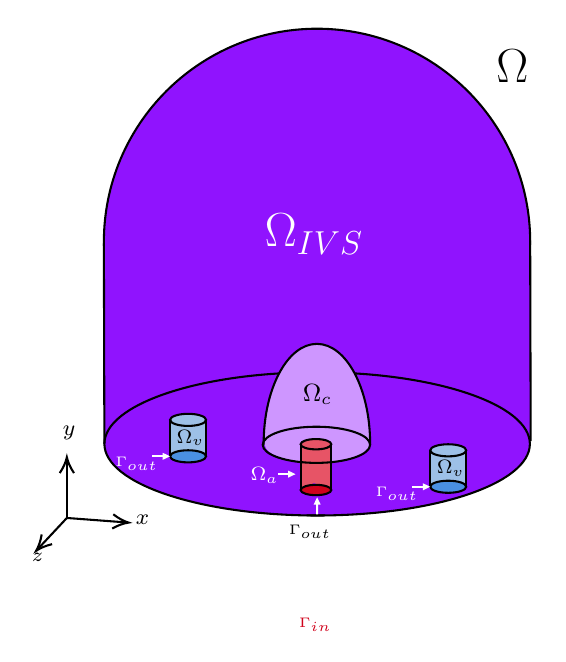
\begin{tikzpicture}[x=0.75pt,y=0.75pt,yscale=-1,xscale=1]
%uncomment if require: \path (0,300); %set diagram left start at 0, and has height of 300

%Shape: Polygon [id:ds01690740321670181] 
\draw  [draw opacity=0][fill={rgb, 255:red, 144; green, 19; blue, 254 }  ,fill opacity=1 ] (249.39,123.24) -- (249.64,219.89) -- (149,187.3) -- (44.25,221.25) -- (44,124.6) -- cycle ;
%Shape: Ellipse [id:dp07097539184655921] 
\draw  [fill={rgb, 255:red, 144; green, 19; blue, 254 }  ,fill opacity=1 ] (44.25,221.25) .. controls (44.25,202.2) and (90.14,186.75) .. (146.75,186.75) .. controls (203.36,186.75) and (249.25,202.2) .. (249.25,221.25) .. controls (249.25,240.3) and (203.36,255.75) .. (146.75,255.75) .. controls (90.14,255.75) and (44.25,240.3) .. (44.25,221.25) -- cycle ;
%Shape: Arc [id:dp2751562142003694] 
\draw  [draw opacity=0][fill={rgb, 255:red, 206; green, 150; blue, 255 }  ,fill opacity=1 ] (120.98,221.7) .. controls (120.98,221.54) and (120.98,221.37) .. (120.98,221.21) .. controls (120.98,194.62) and (132.46,173.06) .. (146.63,173.06) .. controls (160.79,173.06) and (172.28,194.62) .. (172.28,221.21) .. controls (172.28,221.37) and (172.28,221.53) .. (172.28,221.69) -- (146.63,221.21) -- cycle ; \draw   (120.98,221.7) .. controls (120.98,221.54) and (120.98,221.37) .. (120.98,221.21) .. controls (120.98,194.62) and (132.46,173.06) .. (146.63,173.06) .. controls (160.79,173.06) and (172.28,194.62) .. (172.28,221.21) .. controls (172.28,221.37) and (172.28,221.53) .. (172.28,221.69) ;  
%Shape: Polygon [id:ds05551048064302422] 
\draw  [draw opacity=0][fill={rgb, 255:red, 157; green, 192; blue, 231 }  ,fill opacity=1 ] (209.9,227.26) -- (218.57,224.34) -- (218.57,241.91) -- (209.9,238.99) -- (201.24,241.91) -- (201.24,224.34) -- cycle ;
%Straight Lines [id:da2434758497711771] 
\draw    (26.17,229.67) -- (26.17,256.94) ;
\draw [shift={(26.17,227.67)}, rotate = 90] [color={rgb, 255:red, 0; green, 0; blue, 0 }  ][line width=0.75]    (7.65,-3.43) .. controls (4.86,-1.61) and (2.31,-0.47) .. (0,0) .. controls (2.31,0.47) and (4.86,1.61) .. (7.65,3.43)   ;
%Straight Lines [id:da34708087552976474] 
\draw    (53.92,259.02) -- (26.17,256.94) ;
\draw [shift={(55.92,259.17)}, rotate = 184.27] [color={rgb, 255:red, 0; green, 0; blue, 0 }  ][line width=0.75]    (7.65,-3.43) .. controls (4.86,-1.61) and (2.31,-0.47) .. (0,0) .. controls (2.31,0.47) and (4.86,1.61) .. (7.65,3.43)   ;
%Straight Lines [id:da30935515392198853] 
\draw    (12.7,271.34) -- (26.17,256.94) ;
\draw [shift={(11.33,272.8)}, rotate = 313.09] [color={rgb, 255:red, 0; green, 0; blue, 0 }  ][line width=0.75]    (7.65,-3.43) .. controls (4.86,-1.61) and (2.31,-0.47) .. (0,0) .. controls (2.31,0.47) and (4.86,1.61) .. (7.65,3.43)   ;
%Shape: Arc [id:dp4353496030990409] 
\draw  [draw opacity=0][fill={rgb, 255:red, 144; green, 19; blue, 254 }  ,fill opacity=1 ] (44.01,125.8) .. controls (44,125.17) and (44,124.55) .. (44,123.92) .. controls (44,67.2) and (89.98,21.22) .. (146.7,21.22) .. controls (203.42,21.22) and (249.4,67.2) .. (249.4,123.92) .. controls (249.4,124.42) and (249.39,124.91) .. (249.39,125.41) -- (146.7,123.92) -- cycle ; \draw   (44.01,125.8) .. controls (44,125.17) and (44,124.55) .. (44,123.92) .. controls (44,67.2) and (89.98,21.22) .. (146.7,21.22) .. controls (203.42,21.22) and (249.4,67.2) .. (249.4,123.92) .. controls (249.4,124.42) and (249.39,124.91) .. (249.39,125.41) ;  
%Straight Lines [id:da13806152488339984] 
\draw    (44,124.6) -- (44.25,221.25) ;
%Straight Lines [id:da6383479755639994] 
\draw    (249.39,123.24) -- (249.64,219.89) ;
%Shape: Ellipse [id:dp9307891644906987] 
\draw  [fill={rgb, 255:red, 157; green, 192; blue, 231 }  ,fill opacity=1 ] (201.24,224.34) .. controls (201.24,222.73) and (205.12,221.43) .. (209.9,221.43) .. controls (214.69,221.43) and (218.57,222.73) .. (218.57,224.34) .. controls (218.57,225.95) and (214.69,227.26) .. (209.9,227.26) .. controls (205.12,227.26) and (201.24,225.95) .. (201.24,224.34) -- cycle ;
%Shape: Ellipse [id:dp9565465123212877] 
\draw  [fill={rgb, 255:red, 74; green, 144; blue, 226 }  ,fill opacity=1 ] (201.24,241.91) .. controls (201.24,240.29) and (205.12,238.99) .. (209.9,238.99) .. controls (214.69,238.99) and (218.57,240.29) .. (218.57,241.91) .. controls (218.57,243.52) and (214.69,244.82) .. (209.9,244.82) .. controls (205.12,244.82) and (201.24,243.52) .. (201.24,241.91) -- cycle ;
%Shape: Ellipse [id:dp9395551579921961] 
\draw  [draw opacity=0][fill={rgb, 255:red, 206; green, 150; blue, 255 }  ,fill opacity=1 ] (121.57,221.69) .. controls (121.57,216.98) and (132.92,213.16) .. (146.92,213.16) .. controls (160.93,213.16) and (172.28,216.98) .. (172.28,221.69) .. controls (172.28,226.4) and (160.93,230.23) .. (146.92,230.23) .. controls (132.92,230.23) and (121.57,226.4) .. (121.57,221.69) -- cycle ;
%Straight Lines [id:da37394575581946365] 
\draw    (218.57,224.34) -- (218.57,241.91) ;
%Straight Lines [id:da5923482443180503] 
\draw    (201.24,224.34) -- (201.24,241.91) ;
%Shape: Polygon [id:ds36655981362937773] 
\draw  [draw opacity=0][fill={rgb, 255:red, 231; green, 84; blue, 102 }  ,fill opacity=1 ] (146.19,223.89) -- (153.57,221.41) -- (153.57,243.47) -- (145.22,240.09) -- (138.8,243.47) -- (138.8,221.41) -- cycle ;
%Straight Lines [id:da12421975552257325] 
\draw    (138.8,221.41) -- (138.8,243.47) ;
%Straight Lines [id:da06433371565445012] 
\draw    (153.57,221.41) -- (153.57,243.47) ;
%Shape: Ellipse [id:dp9306496239950879] 
\draw  [fill={rgb, 255:red, 231; green, 84; blue, 102 }  ,fill opacity=1 ] (138.8,221.41) .. controls (138.8,220.04) and (142.11,218.92) .. (146.19,218.92) .. controls (150.26,218.92) and (153.57,220.04) .. (153.57,221.41) .. controls (153.57,222.78) and (150.26,223.89) .. (146.19,223.89) .. controls (142.11,223.89) and (138.8,222.78) .. (138.8,221.41) -- cycle ;
%Straight Lines [id:da9919027107135354] 
\draw [color={rgb, 255:red, 255; green, 255; blue, 255 }  ,draw opacity=1 ]   (133.33,235.83) -- (127.67,235.83) ;
\draw [shift={(136.33,235.83)}, rotate = 180] [fill={rgb, 255:red, 255; green, 255; blue, 255 }  ,fill opacity=1 ][line width=0.08]  [draw opacity=0] (3.57,-1.72) -- (0,0) -- (3.57,1.72) -- cycle    ;
%Shape: Ellipse [id:dp6340587055082747] 
\draw   (120.53,221.69) .. controls (120.53,216.88) and (132.11,212.98) .. (146.4,212.98) .. controls (160.69,212.98) and (172.28,216.88) .. (172.28,221.69) .. controls (172.28,226.5) and (160.69,230.4) .. (146.4,230.4) .. controls (132.11,230.4) and (120.53,226.5) .. (120.53,221.69) -- cycle ;
%Straight Lines [id:da4747494457620296] 
\draw [color={rgb, 255:red, 255; green, 255; blue, 255 }  ,draw opacity=1 ]   (198.24,241.91) -- (192.57,241.91) ;
\draw [shift={(201.24,241.91)}, rotate = 180] [fill={rgb, 255:red, 255; green, 255; blue, 255 }  ,fill opacity=1 ][line width=0.08]  [draw opacity=0] (3.57,-1.72) -- (0,0) -- (3.57,1.72) -- cycle    ;
%Shape: Polygon [id:ds6448294514764339] 
\draw  [draw opacity=0][fill={rgb, 255:red, 157; green, 192; blue, 231 }  ,fill opacity=1 ] (84.57,212.59) -- (93.24,209.68) -- (93.24,227.24) -- (84.57,224.32) -- (75.9,227.24) -- (75.9,209.68) -- cycle ;
%Shape: Ellipse [id:dp5042958695035071] 
\draw  [fill={rgb, 255:red, 157; green, 192; blue, 231 }  ,fill opacity=1 ] (75.9,209.68) .. controls (75.9,208.07) and (79.78,206.76) .. (84.57,206.76) .. controls (89.36,206.76) and (93.24,208.07) .. (93.24,209.68) .. controls (93.24,211.29) and (89.36,212.59) .. (84.57,212.59) .. controls (79.78,212.59) and (75.9,211.29) .. (75.9,209.68) -- cycle ;
%Shape: Ellipse [id:dp621045676508921] 
\draw  [fill={rgb, 255:red, 74; green, 144; blue, 226 }  ,fill opacity=1 ] (75.9,227.24) .. controls (75.9,225.63) and (79.78,224.32) .. (84.57,224.32) .. controls (89.36,224.32) and (93.24,225.63) .. (93.24,227.24) .. controls (93.24,228.85) and (89.36,230.16) .. (84.57,230.16) .. controls (79.78,230.16) and (75.9,228.85) .. (75.9,227.24) -- cycle ;
%Straight Lines [id:da6241652370301061] 
\draw    (93.24,209.68) -- (93.24,227.24) ;
%Straight Lines [id:da7595036939515529] 
\draw    (75.9,209.68) -- (75.9,227.24) ;
%Straight Lines [id:da6580144119581173] 
\draw [color={rgb, 255:red, 255; green, 255; blue, 255 }  ,draw opacity=1 ]   (72.9,227.24) -- (67.24,227.24) ;
\draw [shift={(75.9,227.24)}, rotate = 180] [fill={rgb, 255:red, 255; green, 255; blue, 255 }  ,fill opacity=1 ][line width=0.08]  [draw opacity=0] (3.57,-1.72) -- (0,0) -- (3.57,1.72) -- cycle    ;
%Straight Lines [id:da516421428956964] 
\draw [color={rgb, 255:red, 255; green, 255; blue, 255 }  ,draw opacity=1 ]   (146.76,249.98) -- (146.75,255.75) ;
\draw [shift={(146.76,246.98)}, rotate = 90.08] [fill={rgb, 255:red, 255; green, 255; blue, 255 }  ,fill opacity=1 ][line width=0.08]  [draw opacity=0] (3.57,-1.72) -- (0,0) -- (3.57,1.72) -- cycle    ;
%Shape: Arc [id:dp001845141988116028] 
\draw  [draw opacity=0] (150.65,255.68) .. controls (149.31,255.7) and (147.97,255.71) .. (146.63,255.71) .. controls (144.98,255.71) and (143.34,255.7) .. (141.7,255.67) -- (146.63,221.21) -- cycle ; \draw   (150.65,255.68) .. controls (149.31,255.7) and (147.97,255.71) .. (146.63,255.71) .. controls (144.98,255.71) and (143.34,255.7) .. (141.7,255.67) ;  
%Shape: Ellipse [id:dp7362360871362295] 
\draw  [fill={rgb, 255:red, 208; green, 2; blue, 27 }  ,fill opacity=1 ] (138.8,243.47) .. controls (138.8,242.1) and (142.11,240.98) .. (146.19,240.98) .. controls (150.26,240.98) and (153.57,242.1) .. (153.57,243.47) .. controls (153.57,244.84) and (150.26,245.95) .. (146.19,245.95) .. controls (142.11,245.95) and (138.8,244.84) .. (138.8,243.47) -- cycle ;

% Text Node
\draw (27.27,221.01) node [anchor=south] [inner sep=0.75pt]  [font=\footnotesize]  {$y$};
% Text Node
\draw (57.88,257.72) node [anchor=west] [inner sep=0.75pt]  [font=\footnotesize]  {$x$};
% Text Node
\draw (7.79,276.08) node [anchor=west] [inner sep=0.75pt]  [font=\scriptsize]  {$z$};
% Text Node
\draw (145.32,120.23) node  [font=\LARGE,color={rgb, 255:red, 255; green, 255; blue, 255 }  ,opacity=1 ]  {$\Omega _{\text{IVS}}$};
% Text Node
\draw (146.92,197.43) node  [font=\small,color={rgb, 255:red, 0; green, 0; blue, 0 }  ,opacity=1 ]  {$\Omega _{\text{c}}$};
% Text Node
\draw (129.63,236.34) node [anchor=east] [inner sep=0.75pt]  [font=\scriptsize,color={rgb, 255:red, 255; green, 255; blue, 255 }  ,opacity=1 ]  {$\Omega _{\text{a}}$};
% Text Node
\draw (211.09,233.02) node  [font=\scriptsize,color={rgb, 255:red, 0; green, 0; blue, 0 }  ,opacity=1 ]  {$\Omega _{\text{v}}$};
% Text Node
\draw (240.82,39.23) node  [font=\LARGE,color={rgb, 255:red, 0; green, 0; blue, 0 }  ,opacity=1 ]  {$\Omega $};
% Text Node
\draw (145.93,303.53) node [anchor=north] [inner sep=0.75pt]  [font=\tiny,color={rgb, 255:red, 208; green, 2; blue, 27 }  ,opacity=1 ]  {$\Gamma _{\text{in}}$};
% Text Node
\draw (196.83,240.77) node [anchor=north east] [inner sep=0.75pt]  [font=\tiny,color={rgb, 255:red, 255; green, 255; blue, 255 }  ,opacity=1 ]  {$\Gamma _{\text{out}}$};
% Text Node
\draw (85.75,218.35) node  [font=\scriptsize,color={rgb, 255:red, 0; green, 0; blue, 0 }  ,opacity=1 ]  {$\Omega _{\text{v}}$};
% Text Node
\draw (71.5,226.1) node [anchor=north east] [inner sep=0.75pt]  [font=\tiny,color={rgb, 255:red, 255; green, 255; blue, 255 }  ,opacity=1 ]  {$\Gamma _{\text{out}}$};
% Text Node
\draw (155,268.36) node [anchor=south east] [inner sep=0.75pt]  [font=\tiny,color={rgb, 255:red, 0; green, 0; blue, 0 }  ,opacity=1 ]  {$\Gamma _{\text{out}}$};


\end{tikzpicture}

        %             \caption{}
        %             \label{fig:box-circle-3d:regions}
        %         \end{subfigure}
        %         \caption{Not to scale. (a) Diagram illustrating a simple 3D placentone geometry with dimensions. Red shows the inlet location and blue shows outlet locations. (b) Diagram illustrating subdomains with $\Omega$.}
        %         \label{fig:box-circle-3d}
        %     \end{figure}

    \section{Blood flow model} \label{sec:modelling:blood-flow}        
        Previous authors using macro-scale models for maternal blood flow take flow through the villous tree as porous flow, and to treat other flows as `free' flow. Here, we will introduce a model that respects this approach, and make comparisons to other popular choices in the literature \cite{lecarpentierComputationalFluidDynamic2016,chernyavskyMathematicalModelIntervillous2010,meklerImpactTissuePorosity2022,erianMaternalPlacentalBlood1977,saghianAssociationPlacentalJets2017} through \S\ref{sec:modelling:blood-flow:s+b}--\ref{sec:modelling:blood-flow:ns+nsb}.
            
        One of the main contributions of this thesis is to use the Navier-Stokes-Darcy (NSD) equations to model maternal blood flow on a 2D placenta geometry. Whilst there is work that uses NSD and related models \cite{angotPenalizationMethodTake1999,fuchsbergerIncorporationObstaclesFluid2022,engelsFluSINovelParallel2016,jiaModelingAnalysisCarbonate2021}, as far as we are aware there is only one work that uses a single Navier-Stokes-type PDE to model flow in the context of the placenta \cite{meklerImpactTissuePorosity2022}. This approach is advantageous for the numerical methods we will employ, gives a physiologically sensible transition region between `free' and porous flow, and avoids non-physical boundary layers that may occur when coupling, for example, the Navier-Stokes and Brinkman equations \cite{brinkmanCalculationViscousForce1949}. To be clear, our model of maternal blood flow is: find $\vec{u}, p$ such that
        \begin{subequations}
            \begin{align}
                \begin{split}
                    \rho \pdv{\vec{u}}{t} + \Psi \frac{\mu}{k} \vec{u} + \rho (\vec{u} \cdot \vec{\nabla}) \vec{u} - \mu \nabla^2 \vec{u} + \vec{\nabla} p = \vec{f}_\text{f} &~ \text{in } \Omega,
                    \label{eq:nsb:momentum}
                \end{split}\\
                \begin{split}
                    \vec{\nabla} \cdot \vec{u} = 0 &~ \text{in } \Omega,
                    \label{eq:nsb:incompressibility}%
                \end{split}%
            \end{align}%
            \label{eq:nsb}%
        \end{subequations}%
        where the problem is supplemented with a suitable initial condition and boundary conditions (to be given in \S\ref{sec:modelling:blood-flow:boundary-conditions}), $\rho$ is the density of the fluid, $\mu$ is the dynamic viscosity, $\vec{f}_\text{f}$ is a body force acting on the flow, and the coefficient of the reaction term varies spatially, i.e., $\Psi(\vec{x}) \frac{\mu}{k}$. We assign $\Psi = 1$ in areas of villous tree, $\Psi = 0$ in areas of no villous tree, with a smooth transition on the region in between. The shape of this smooth transition follows a $\tanh$ profile. Figure \ref{fig:permeability} illustrates an example of the profile of $\Psi$ in the placentone geometry, and Appendix \ref{sec:smooth-transition} contains the details on the precise definition of this function.

        \begin{figure}
            \centering
            

\tikzset{every picture/.style={line width=0.75pt}} %set default line width to 0.75pt        

\begin{tikzpicture}[x=0.75pt,y=0.75pt,yscale=-1,xscale=1]
%uncomment if require: \path (0,300); %set diagram left start at 0, and has height of 300

%Shape: Rectangle [id:dp05948589068926391] 
\draw  [color={rgb, 255:red, 144; green, 19; blue, 254 }  ,draw opacity=1 ][fill={rgb, 255:red, 255; green, 255; blue, 255 }  ,fill opacity=1 ][line width=2.25] [blur shadow={shadow xshift=0pt,shadow yshift=0pt, shadow blur radius=1.5pt, shadow blur steps=4 ,shadow opacity=100}] (23,74.5) -- (160,74.5) -- (160,218) -- (23,218) -- cycle ;
%Image [id:dp5741033059414491] 
\draw (279.44,145.67) node  {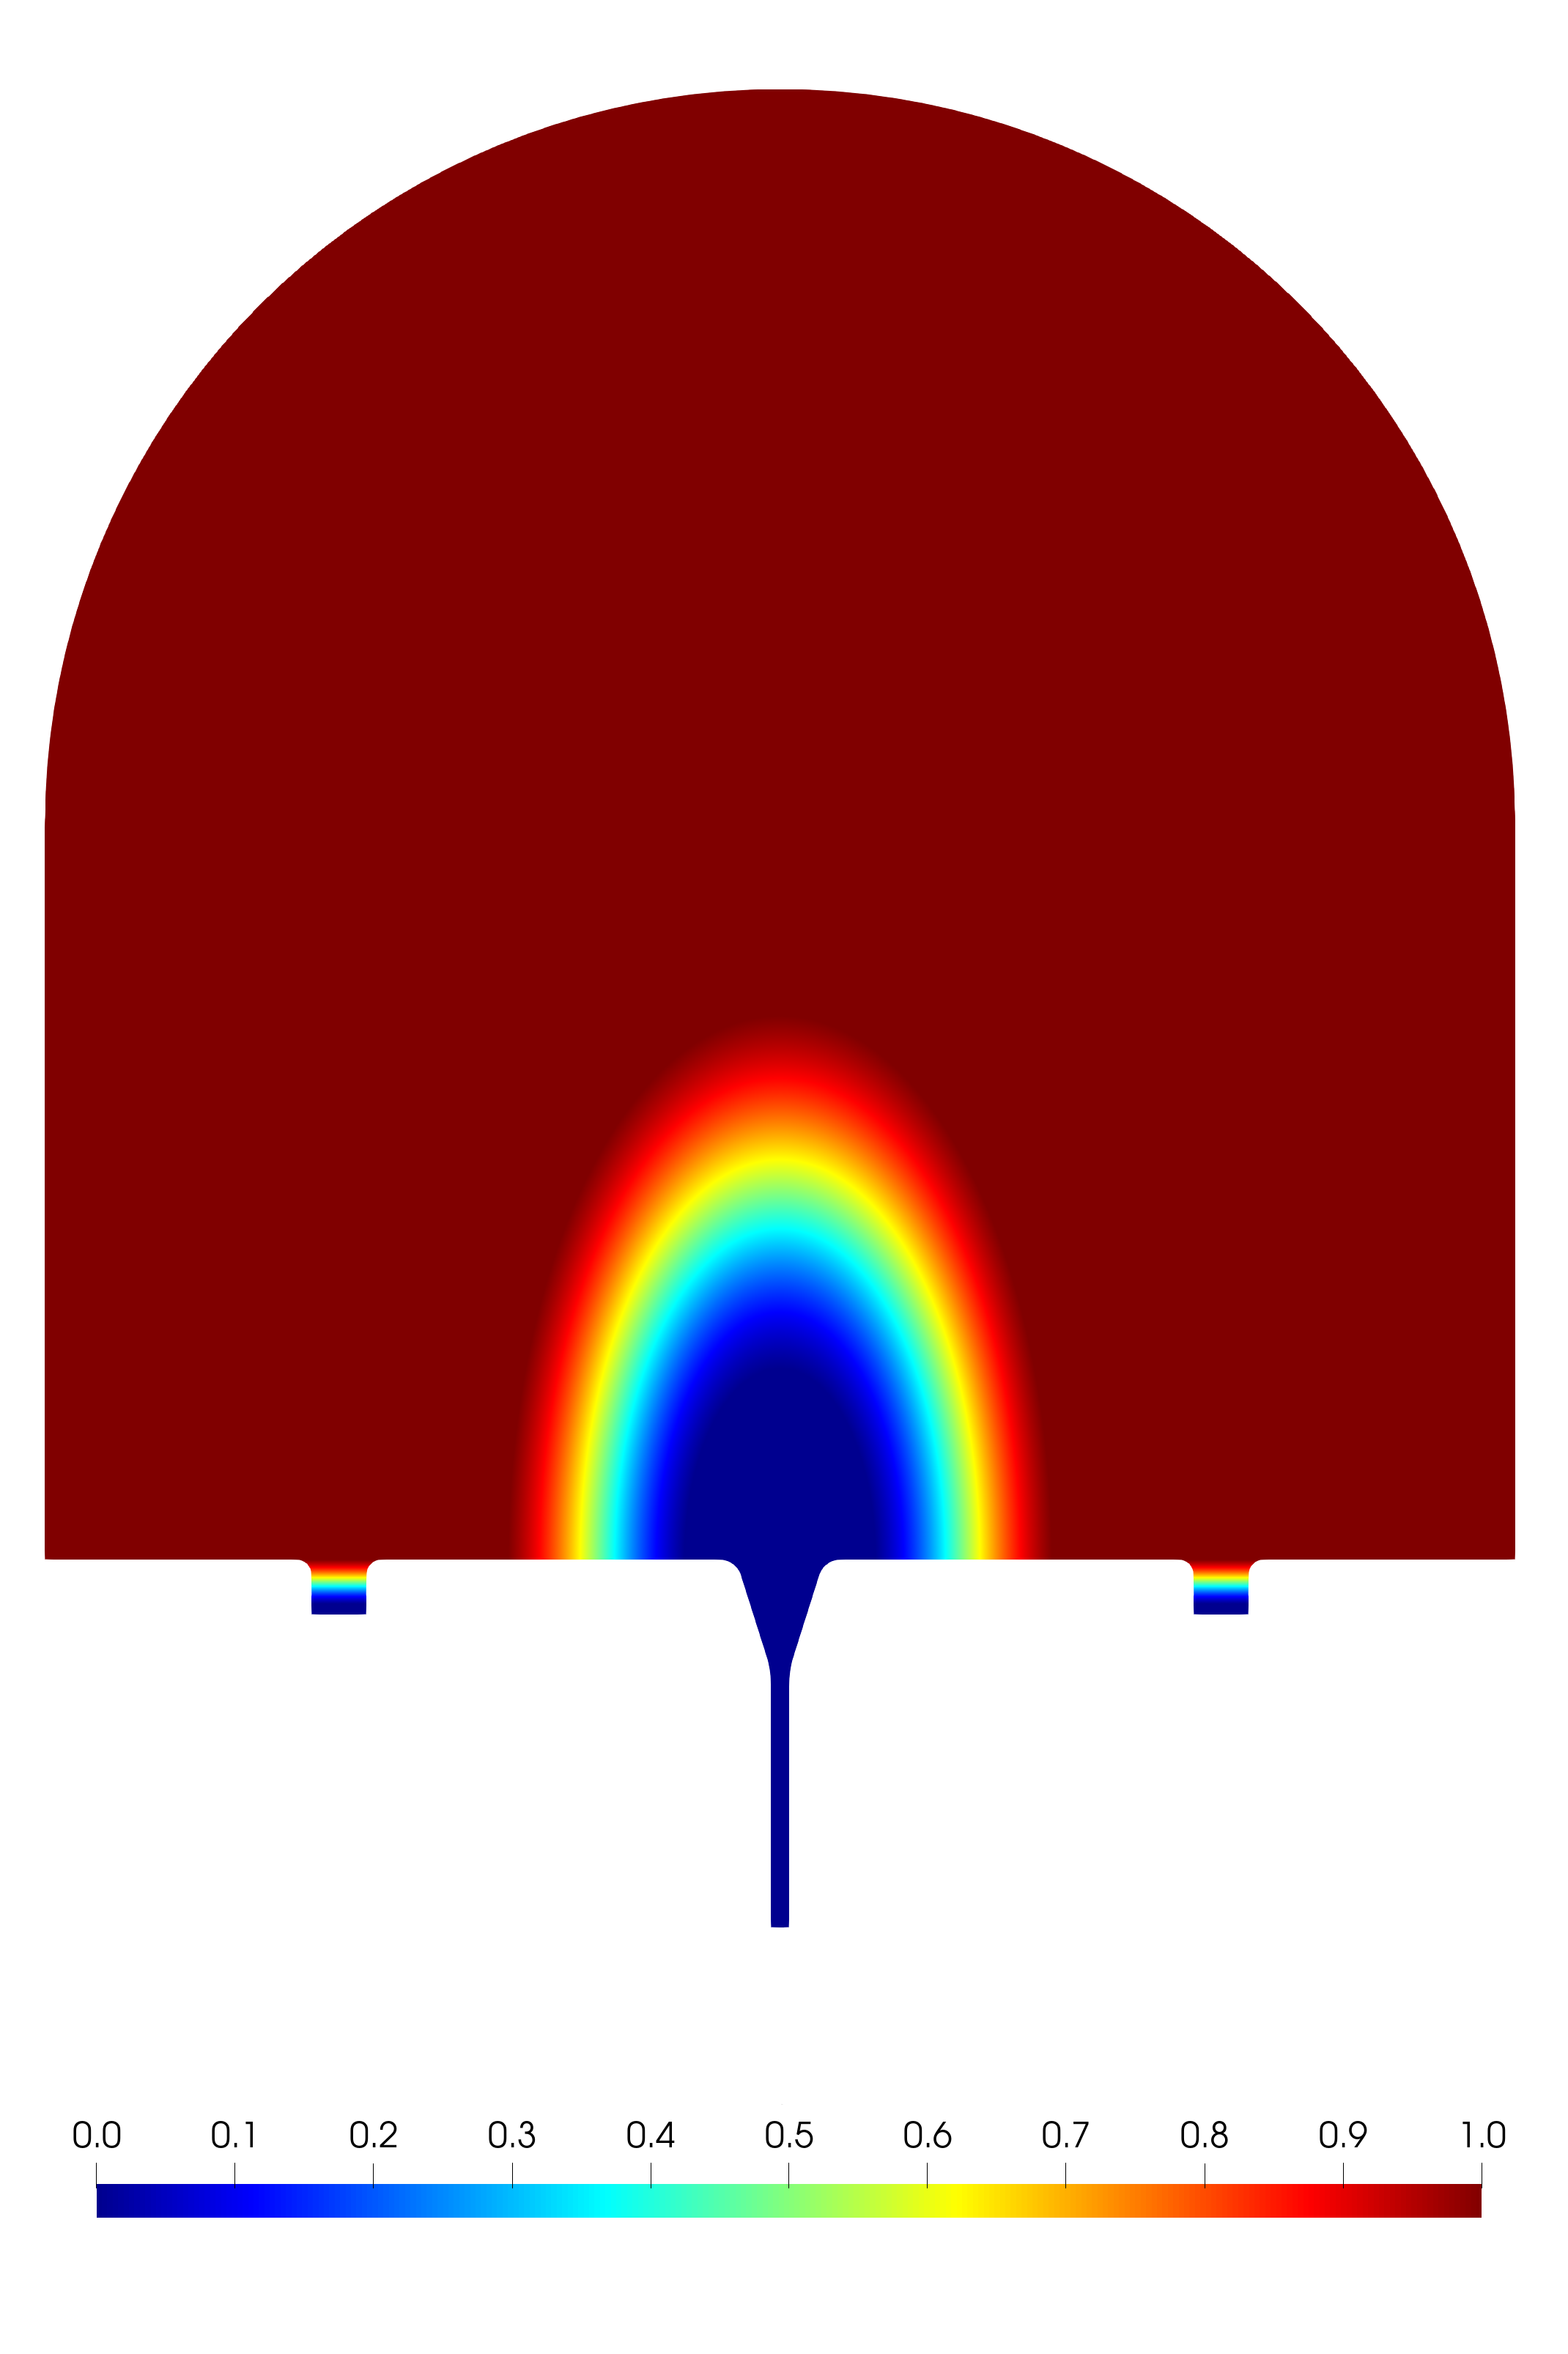
\includegraphics[width=142.91pt,height=214.5pt]{diagrams/results-modelling/velocity-transport/meshandsoln_cg_permeability_placenta_nsb_permeability-linear.png}};
%Image [id:dp5031667319380262] 
\draw (90.5,171.72) node  {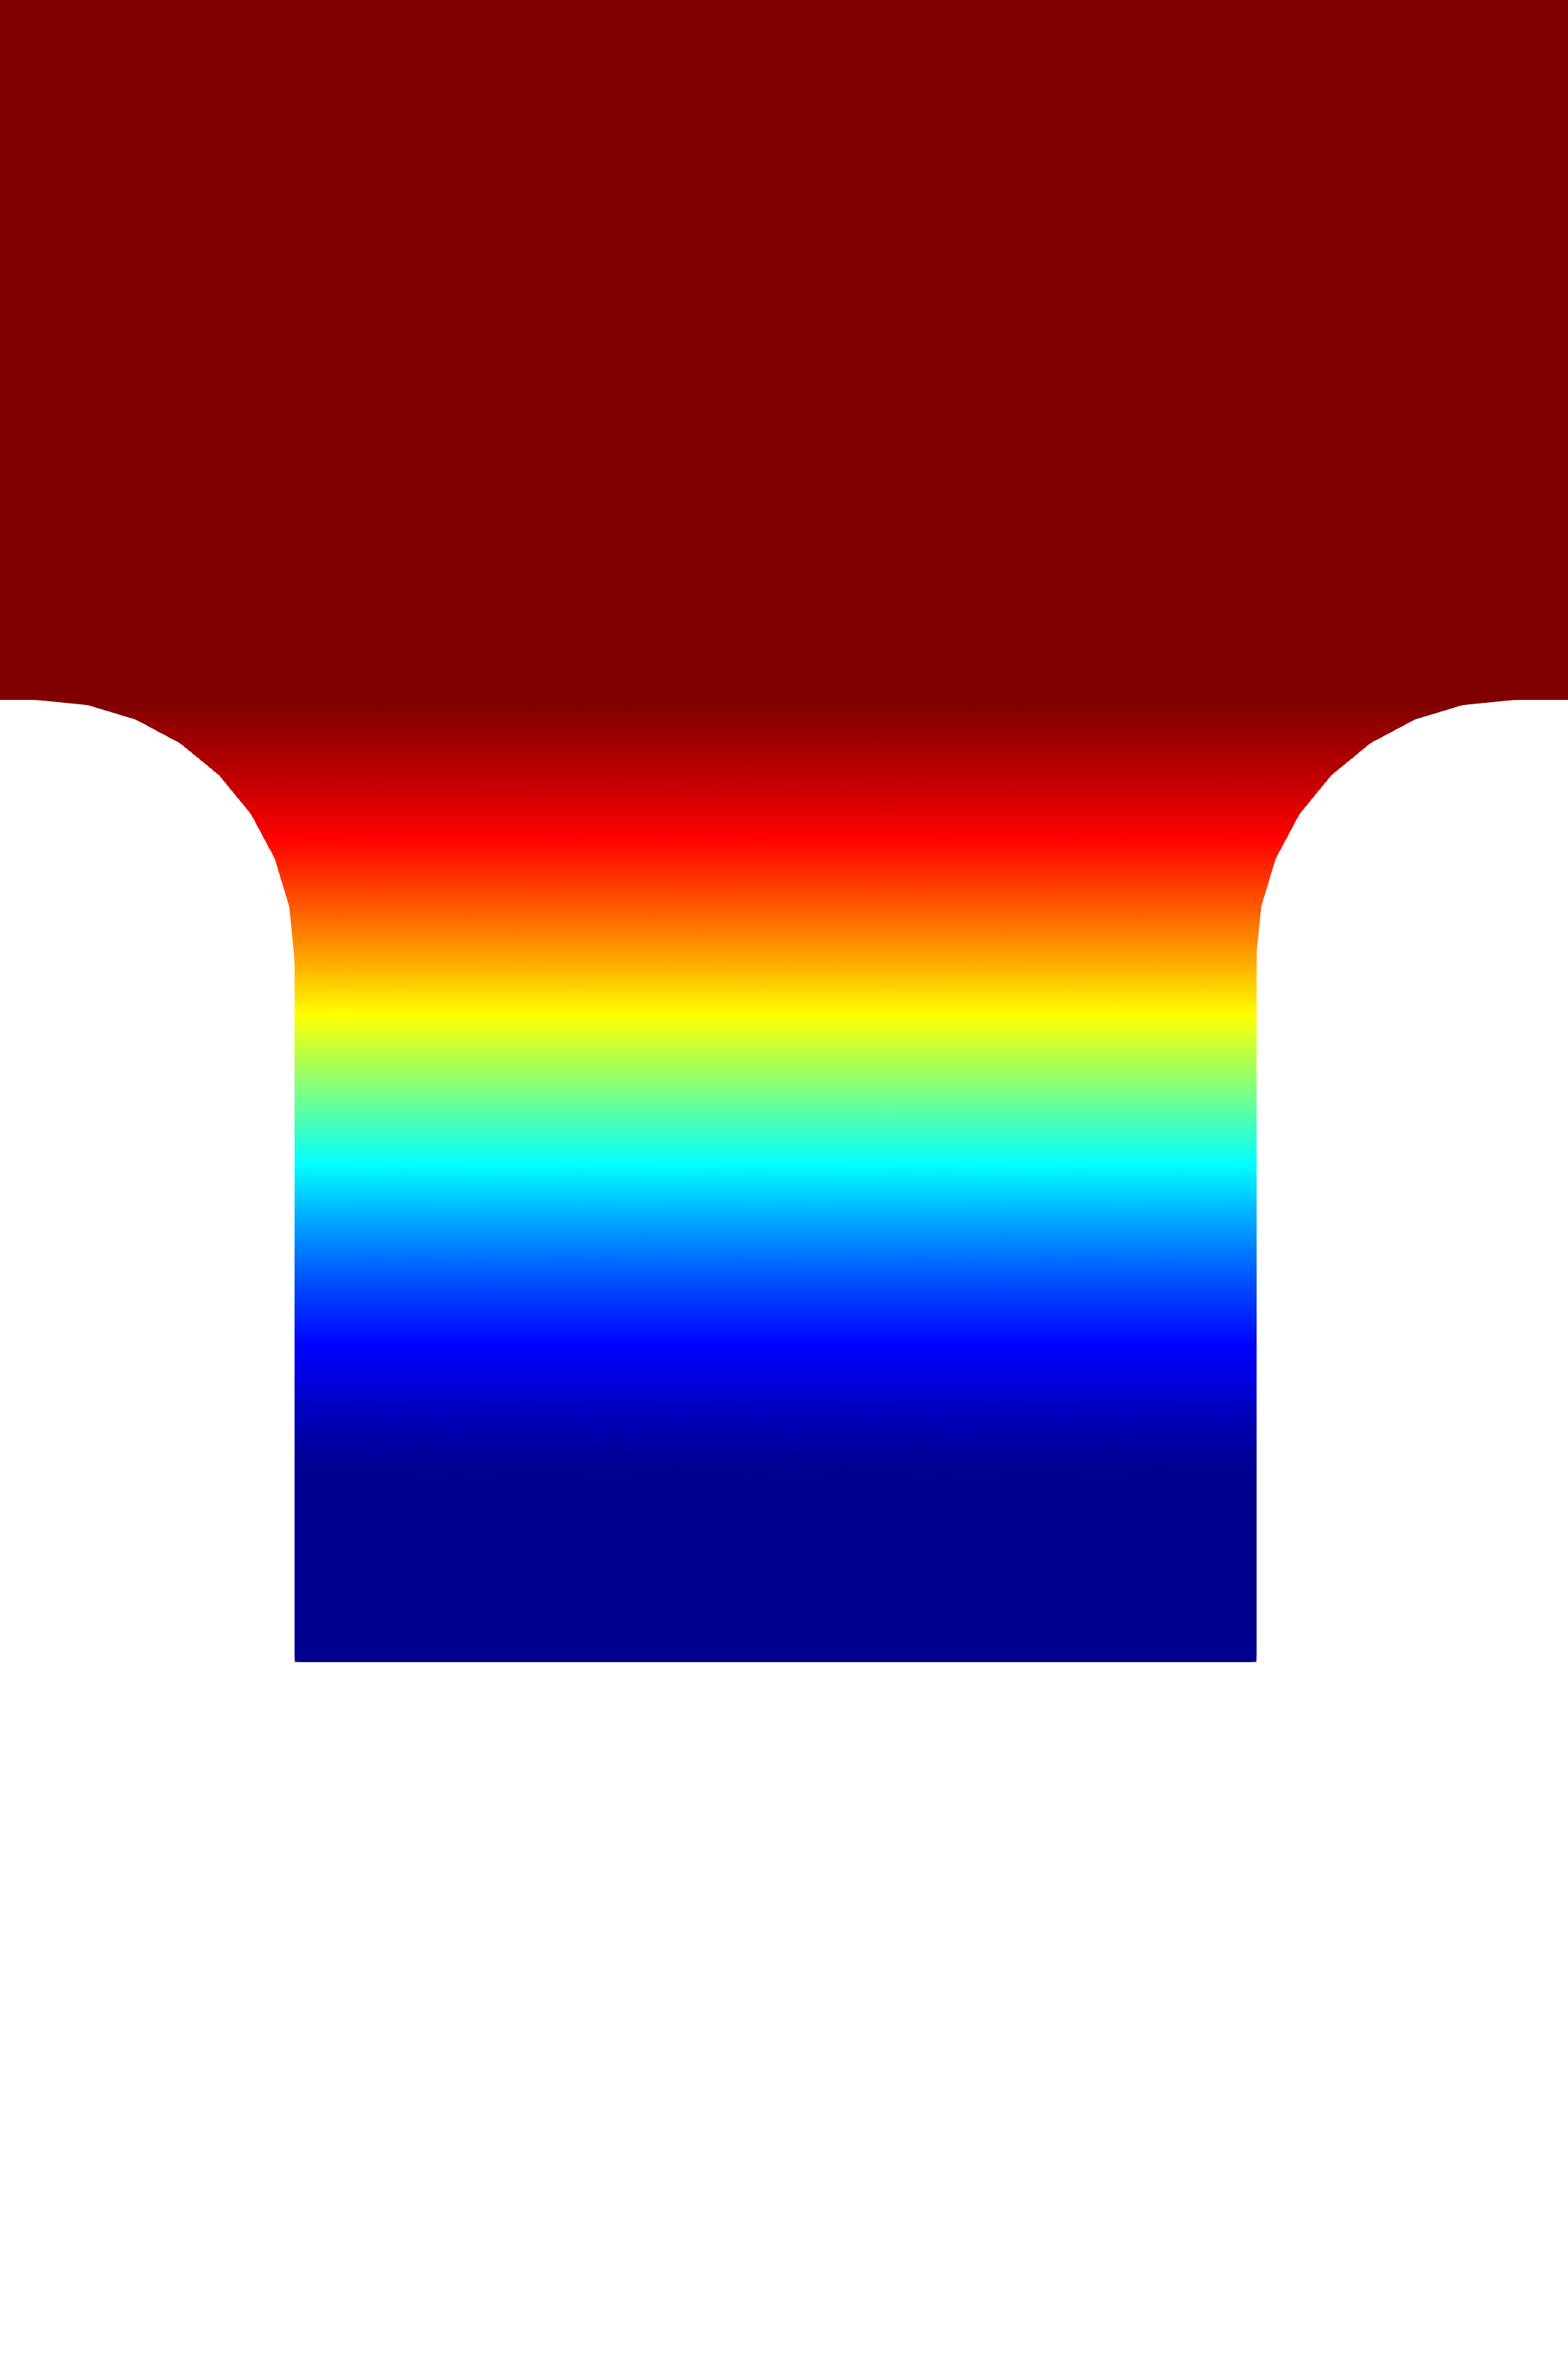
\includegraphics[width=82.5pt,height=123.83pt]{diagrams/results-modelling/velocity-transport/meshandsoln_cg_permeability_placenta_nsb_permeability-linear_vein.png}};
%Shape: Polygon [id:ds7395586031334473] 
\draw  [fill={rgb, 255:red, 155; green, 155; blue, 155 }  ,fill opacity=0.2 ] (421.25,250.25) -- (317,245.5) -- (317,120) -- (421.25,23) -- cycle ;
%Shape: Rectangle [id:dp1357774358505115] 
\draw   (240.75,120) -- (317,120) -- (317,245.5) -- (240.75,245.5) -- cycle ;
%Shape: Rectangle [id:dp02134536760375405] 
\draw  [color={rgb, 255:red, 144; green, 19; blue, 254 }  ,draw opacity=1 ][fill={rgb, 255:red, 255; green, 255; blue, 255 }  ,fill opacity=1 ][line width=2.25] [blur shadow={shadow xshift=0pt,shadow yshift=0pt, shadow blur radius=1.5pt, shadow blur steps=4 ,shadow opacity=100}] (421.25,23) -- (576.5,23) -- (576.5,250.5) -- (421.25,250.5) -- cycle ;
%Image [id:dp27582567302078576] 
\draw (497.74,131.58) node  {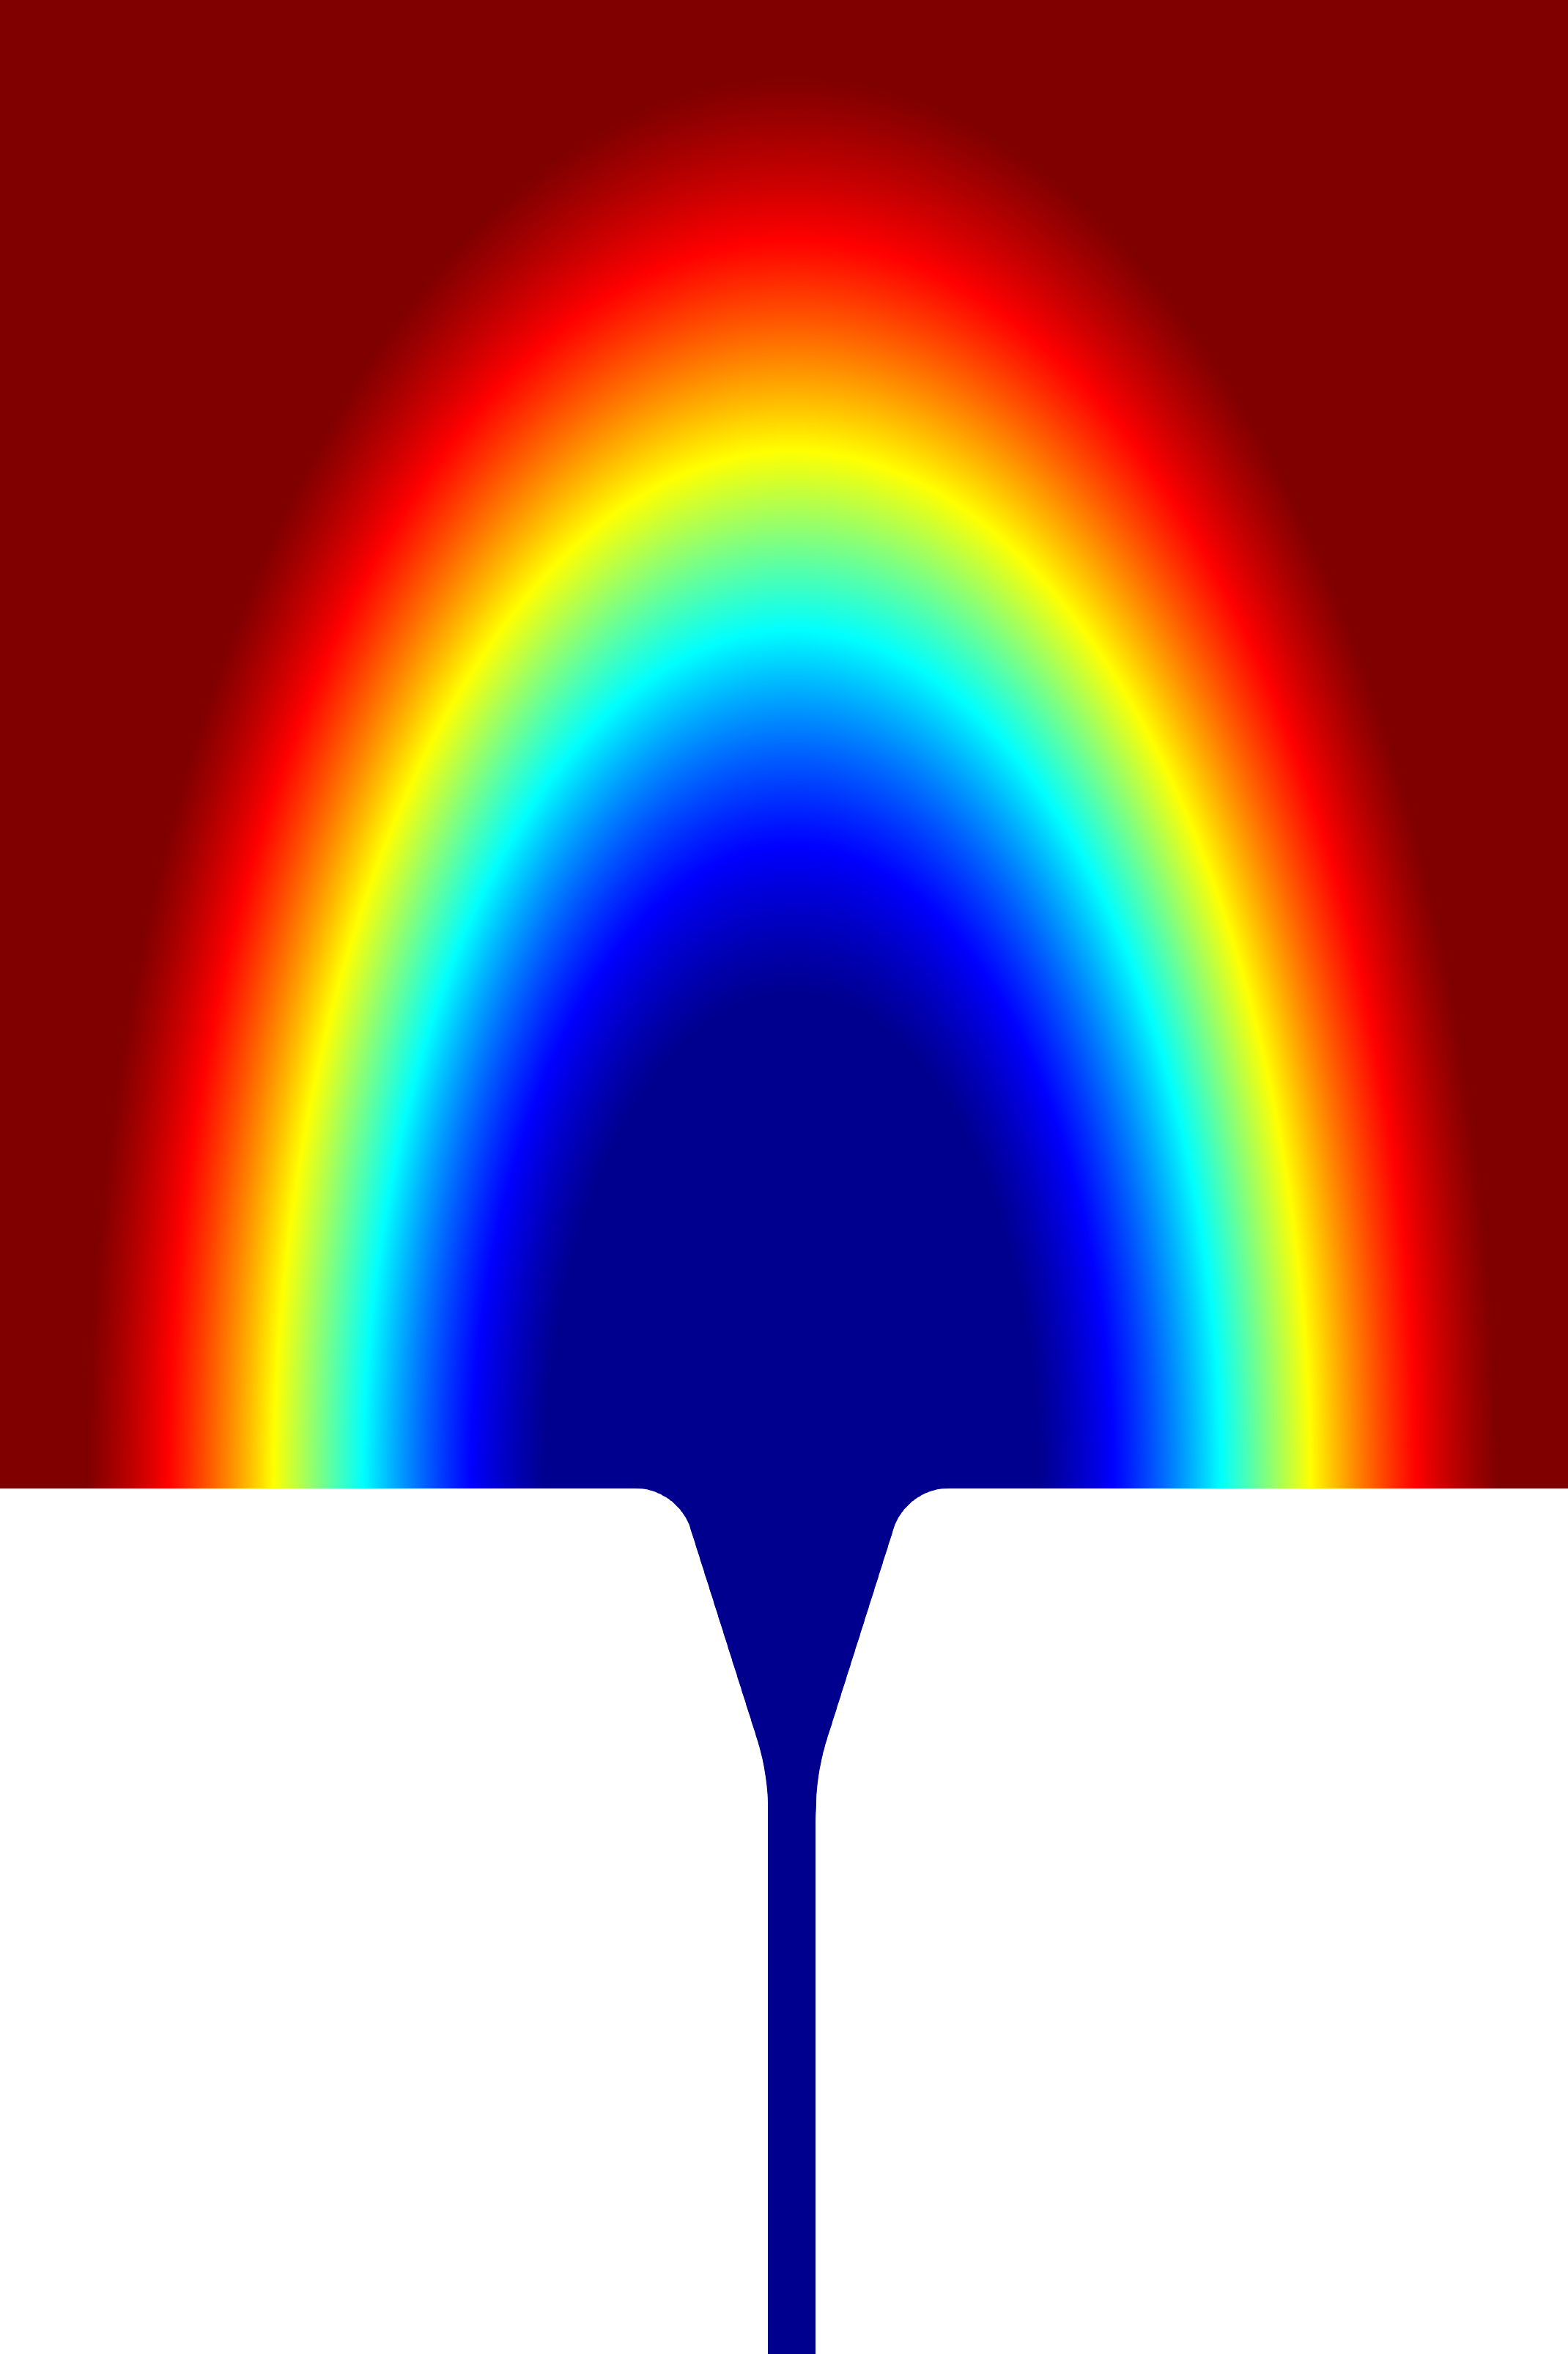
\includegraphics[width=101.85pt,height=152.88pt]{diagrams/results-modelling/velocity-transport/meshandsoln_cg_permeability_placenta_nsb_permeability-linear_cavity.png}};
%Shape: Polygon [id:ds4671748834121485] 
\draw  [fill={rgb, 255:red, 155; green, 155; blue, 155 }  ,fill opacity=0.2 ] (217.75,202.5) -- (160,218) -- (160,74.5) -- (217.75,186.5) -- cycle ;
%Shape: Rectangle [id:dp28400651386966036] 
\draw   (217.75,186.5) -- (231,186.5) -- (231,202.5) -- (217.75,202.5) -- cycle ;




\end{tikzpicture}

            \caption{Diagram illustrating $\Psi$ on a placentone as described in \S\ref{sec:modelling:blood-flow}. Blue regions correspond to $\Psi = 0$ and red regions correspond to $\Psi = 1$. The definition of $\Psi$ is formally presented in Appendix \ref{sec:smooth-transition}. The value is dependent upon the subregions of $\Omega$ and transition sizes that are illustrated in Figure \ref{fig:box-circle}.}
            \label{fig:permeability}
        \end{figure}
            
        Through the remainder of \S\ref{sec:modelling:blood-flow}, we will define three alternative blood flow models, as these form common choices in the current literature, and present the boundary conditions and parameters we will use in these problems. Approximations to these problems will then be compared later in \S\ref{sec:numerical-methods:blood-flow-experiments}; for simplicity, these comparisons will consider only the steady-state equations. We will consider:
        \begin{itemize}
            \item \S\ref{sec:modelling:blood-flow:boundary-conditions}: Boundary conditions and model parameters common to all flow problems,
            \item \S\ref{sec:modelling:blood-flow:s+b}: Brinkman in $\Omega_\text{IVS} \cup \Omega_{T^+}$ and Stokes in $\Omega \setminus (\Omega_\text{IVS} \cup \Omega_{T^+})$,
            \item \S\ref{sec:modelling:blood-flow:ns+b}: Brinkman in $\Omega_\text{IVS} \cup \Omega_{T^+}$ and Navier-Stokes in $\Omega \setminus (\Omega_\text{IVS} \cup \Omega_{T^+})$,
            \item \S\ref{sec:modelling:blood-flow:ns+nsb}: Navier-Stokes-Darcy in $\Omega_\text{IVS} \cup \Omega_{T^+}$ and Navier-Stokes in $\Omega \setminus (\Omega_\text{IVS} \cup \Omega_{T^+})$.
        \end{itemize}

        \subsection{Boundary conditions and placenta parameters} \label{sec:modelling:blood-flow:boundary-conditions}        
            \todoitemone{You are missing the scaling of $U$ on the inlet boundary condition.}
            For all velocity model choices, we prescribe the same boundary conditions: a zero Neumann condition on outflow, with parabolic inflow velocity profile, and no velocity slip elsewhere. Boundary conditions are applied of the form
            \begin{subequations}
                \begin{alignat*}{3}
                    \left( \nabla \vec{u} - p \mat{I} \right) \cdot \vec{n} & = \vec{g}_\text{f,N} &&~ \text{on } \Gamma_\text{out}, \\
                    \vec{u} & = \vec{g}_\text{f,D} &&~ \text{on } \Gamma\setminus\Gamma_\text{out},
                \end{alignat*}%
            \end{subequations}%
            where $\Gamma := \partial \Omega$ is labelled in Figures \ref{fig:box-circle:regions} and \ref{fig:inverted-circle-slice-6-flat:regions}, and $\vec{n}(\vec{x})$ is the unit outward-pointing normal at a point $\vec{x}$. The boundary conditions themselves are given by
            \begin{subequations}
                \begin{alignat}{3}
                    \vec{g}_\text{f,D} & = - \frac{R^2 - r^2}{R^2} \vec{n} &&~ \text{on } \Gamma_\text{in},\label{eq:velocity-bcs:dirichlet-parabola}\\
                    \vec{g}_\text{f,N} & = \vec{0} &&~ \text{on } \Gamma_\text{out},\label{eq:velocity-bcs:neumann}\\
                    \vec{g}_\text{f,D} & = \vec{0} &&~ \text{on } \Gamma \setminus (\Gamma_\text{in} \cup \Gamma_\text{out}),\label{eq:velocity-bcs:dirichlet-no-slip}
                \end{alignat}%
                \label{eq:velocity-bcs}%
            \end{subequations}%
            where $\vec{n}$ is the unit outward-pointing normal on $\Gamma_\text{in}$, $r(\vec{x})$ is the distance to from a point $\vec{x}$ to the centre of $\Gamma_\text{in}$, and $R$ is the artery radius.

            Tables \ref{tab:structural-parameters} and \ref{tab:problem-parameters} give lists of parameters used throughout this thesis' analyses, where the nominal values listed are used in all simulations unless otherwise stated.

            \todoitemone{Is the cavity transition width correct? Check. Also add the vein transition width.}
            \begin{table}
                \centering
                \begin{adjustwidth}{-1.5cm}{-1cm}
                    \begin{tabular}{c|c|c|c|c}
                        Parameter & Description & Nominal value & Range & Reference \\
                        \hline
                        $b_1, a_1$ & Axes of central cavity & \qtylist{1e-2;5e-3}{\metre} & — & \cite{lecarpentierComputationalFluidDynamic2016} \\
                        — & Artery location & \qty{2e-2}{\metre} (from side) & — & \cite{chernyavskyMathematicalModelIntervillous2010,lecarpentierComputationalFluidDynamic2016} \\
                        — & Vein location & \qty{8e-3}{\metre} (from side) & — & \cite{chernyavskyMathematicalModelIntervillous2010,lecarpentierComputationalFluidDynamic2016} \\
                        — & Artery width (mouth) & \qty{2.4e-3}{\metre} & \qtyrange{5e-4}{3e-3}{\metre} & \cite{burtonRheologicalPhysiologicalConsequences2009} \\
                        $2r_a$ & Artery width (upstream) & \qty{5e-4}{\metre} & — & \cite{burtonRheologicalPhysiologicalConsequences2009} \\
                        $2r_v$ & Vein width & \qty{1.5e-3}{\metre} & — & — \\
                        $2r^\text{ms}_v$ & Marginal sinus vein width & \qty{3e-3}{\metre} & — & — \\
                        — & Central cavity width & \qty{1e-2}{\metre} & — & \cite{lecarpentierComputationalFluidDynamic2016,chernyavskyMathematicalModelIntervillous2010} \\
                        $\tau$ & Central cavity transition & \qty{2}{\milli\metre} & — & — \\
                        — & Small septal wall heights & \qty{6.90}{\milli\metre} & \qtyrange{5.26}{9.54}{\milli\metre} & \cite{AMANITIS2023e68} \\
                        — & Tall septal wall heights & \qty{14.07}{\milli\metre} & \qtyrange{12.15}{17.75}{\milli\metre} & \cite{AMANITIS2023e68} \\
                        — & Number of arteries (3D) & — & $30$—$150$ & \cite{benirschkePathologyHumanPlacenta2012,chernyavskyMathematicalModelIntervillous2010,burtonRheologicalPhysiologicalConsequences2009} \\
                        — & Number of veins (3D) & — & $50$—$200$ & \cite{chernyavskyMathematicalModelIntervillous2010} \\
                        — & Number of placentones (3D) & — & $30$—$60$ & \cite{benirschkePathologyHumanPlacenta2012,serovRoleMorphologyMathematical2016} \\
                    \end{tabular}
                \end{adjustwidth}
                \caption{Placental structural parameter nominal values and ranges found in the placental literature.}
                \label{tab:structural-parameters}
            \end{table}

            \begin{table}
                \centering
                \begin{adjustwidth}{-1.5cm}{-1cm}
                    \begin{tabular}{c|c|c|c|c}
                        \centering
                        Parameter & Description & Nominal value & Range & Reference \\
                        \hline
                        $L$ & Placentone width & \qty{4e-2}{\metre} & \qtyrange{1e-2}{4e-2}{\metre} & \cite{chernyavskyMathematicalModelIntervillous2010,lecarpentierComputationalFluidDynamic2016} \\
                        $k$ & Villous tree permeability & \qty{1e-8}{\metre^2} & \qtyrange{1e-6}{1e-10}{\metre^2} & \cite{lecarpentierComputationalFluidDynamic2016,chernyavskyMathematicalModelIntervillous2010} \\
                        $\mu$ & Blood viscosity & \qty{4e-3}{\pascal\second} & — & \cite{chernyavskyMathematicalModelIntervillous2010} \\
                        $\rho$ & Blood density & \qty{1e3}{\kilogram\per\metre^3} & — & \cite{chernyavskyMathematicalModelIntervillous2010} \\
                        $D$ & Oxygen diffusivity & \qty{1.667e-5}{\metre^2\per\second} & \qtyrange{1e-5}{1.667e-5}{\metre^2\per\second} & \cite{chernyavskyMathematicalModelIntervillous2010,banerjeeCoupledOxygenTransport2008} \\
                        $R$ & Oxygen uptake & \qty{1.667e-2}{\per\second} & — & \cite{chernyavskyMathematicalModelIntervillous2010} \\
                        — & Artery blood speed (mouth) & \qty{0.1}{\metre\per\second} & \qtyrange{0.037}{0.3}{\metre\per\second} & \cite{burtonRheologicalPhysiologicalConsequences2009,chernyavskyMathematicalModelIntervillous2010,kurjakDopplerAssessmentIntervillous1997,collinsDevelopmentalChangesSpiral2012} \\
                        $U$ & Artery blood speed (upstream) & \qty{0.35}{\metre\per\second}\anote & \qtyrange{0.5}{4}{\metre\per\second} & \cite{burtonRheologicalPhysiologicalConsequences2009,saghianAssociationPlacentalJets2017,chernyavskyMathematicalModelIntervillous2010} \\
                    \end{tabular}
                \end{adjustwidth}
                \caption{Maternal blood parameter nominal values and ranges found in the placental literature. \anote The upstream speed of \qty{0.35}{\metre\per\second} was selected such that flow at the mouth is approximately \qty{0.1}{\metre\per\second}.}
                \label{tab:problem-parameters}
            \end{table}

            \S\ref{sec:modelling:blood-flow:s+b}--\ref{sec:modelling:blood-flow:ns+nsb} will now outline three alternative models of maternal blood flow, taken directly from, or closely related to, those chosen in the literature.

        \subsection{Stokes and Brinkman (S-B)} \label{sec:modelling:blood-flow:s+b}
            We solve Brinkman in the IVS, and Stokes elsewhere: find $\vec{u}, p$ such that
            \begin{subequations}
                \begin{align}
                    \begin{split}
                        \frac{\mu}{k} \vec{u} -\mu\nabla^2 \vec{u} + \vec{\nabla} p = \vec{0} &~ \text{in } \Omega_{\text{IVS}} \cup \Omega_{T^+},
                    \end{split}\\
                    \begin{split}
                        -\mu\nabla^2 \vec{u} + \vec{\nabla} p = \vec{0} &~ \text{in } \Omega \setminus (\Omega_{\text{IVS}} \cup \Omega_{T^+}),
                    \end{split}\\
                    \begin{split}
                        \vec{\nabla} \cdot \vec{u} = 0 &~ \text{in } \Omega,
                    \end{split}%
                \end{align}%
                \label{eq:s-b}%
            \end{subequations}%
            with continuity of velocity and pressure on the cavity-IVS interface, and boundary conditions given in Equation \ref{eq:velocity-bcs}. This is the simplest of the four velocity models, and the only model which is linear everywhere. This model is related to work by \citeauthor{chernyavskyMathematicalModelIntervillous2010} \cite{chernyavskyMathematicalModelIntervillous2010} and \citeauthor{erianMaternalPlacentalBlood1977} \cite{erianMaternalPlacentalBlood1977} who use Darcy's law. We opted to use the Brinkman equation instead of Darcy's law in the porous region for two reasons: firstly, Brinkman captures the drag effects associated with resistance of flow through the villous tree, and secondly, allows for simple application of interface conditions due to both equations being of the same order \cite{brinkmanCalculationViscousForce1949}. 

        \subsection{Navier-Stokes and Brinkman (NS-B)} \label{sec:modelling:blood-flow:ns+b}
            We solve Brinkman in the IVS, and steady-state Navier-Stokes elsewhere: find $\vec{u}, p$ such that
            \begin{subequations}
                \begin{align}
                    \begin{split}
                        \frac{\mu}{k} \vec{u} -\mu\nabla^2 \vec{u} + \vec{\nabla} p = \vec{0} &~ \text{in } \Omega_{\text{IVS}} \cup \Omega_{T^+},
                    \end{split}\\
                    \begin{split}
                        \rho(\vec{u} \cdot \vec{\nabla}) \vec{u} -\mu\nabla^2 \vec{u} + \vec{\nabla} p = \vec{0} &~ \text{in } \Omega \setminus (\Omega_{\text{IVS}} \cup \Omega_{T^+}),
                    \end{split}\\
                    \begin{split}
                        \vec{\nabla} \cdot \vec{u} = 0 &~ \text{in } \Omega,
                    \end{split}%
                \end{align}%
                \label{eq:ns-b}%
            \end{subequations}%
            with continuity of velocity and pressure on the cavity-IVS interface, and boundary conditions given in Equation \ref{eq:velocity-bcs}. This example follows work by \citeauthor{lecarpentierComputationalFluidDynamic2016} \cite{lecarpentierComputationalFluidDynamic2016} who also use Navier-Stokes and Brinkman, and \citeauthor{saghianAssociationPlacentalJets2017} \cite{saghianAssociationPlacentalJets2017} who use a related model of Navier-Stokes and Darcy. This is therefore a useful benchmark model.

        \subsection{Navier-Stokes and Navier-Stokes-Darcy (NS-NSD)} \label{sec:modelling:blood-flow:ns+nsb}
            We solve steady-state Navier-Stokes-Darcy in the IVS, and steady-state Navier-Stokes elsewhere: find $\vec{u}, p$ such that
            \begin{subequations}
                \begin{align}
                    \begin{split}
                        \rho (\vec{u} \cdot \vec{\nabla}) \vec{u} - \mu \nabla^2 \vec{u} + \vec{\nabla} p = \vec{0} &~ \text{in } \Omega_{\text{IVS}} \cup \Omega_{T^+},
                    \end{split}\\
                    \begin{split}
                        \frac{\mu}{k}\vec{u} + \rho (\vec{u} \cdot \vec{\nabla}) \vec{u} - \mu \nabla^2 \vec{u} + \vec{\nabla} p = \vec{0} &~ \text{in } \Omega \setminus (\Omega_{\text{IVS}} \cup \Omega_{T^+}),
                    \end{split}\\
                    \begin{split}
                        \vec{\nabla} \cdot \vec{u} = 0 &~ \text{in } \Omega,
                    \end{split}%
                \end{align}%
                \label{eq:ns-nsb}%
            \end{subequations}%
            with continuity of velocity and pressure on the cavity-IVS interface, and boundary conditions given in Equation \ref{eq:velocity-bcs}. This provides an alternate model to the coupled Navier-Stokes and Brinkman problem in \S\ref{sec:modelling:blood-flow:ns+b}, where the treatment of the interface conditions is more straightforward in the numerical scheme we employ in Chapter \ref{sec:numerical-methods}. We note here that this model is the sharp interface case of NSD.

    \section{Oxygen transport model} \label{sec:modelling:transport}
        We focus on modelling transport of oxygen from maternal blood to fetal blood. We model this using a reaction-advection-diffusion equation for oxygen concentration, where the advective velocity is the blood flow field obtained from \S\ref{sec:modelling:blood-flow} (NSD).
        
        The reaction-advection-diffusion equation is given by: find $c$ such that
        \begin{equation}
            \pdv{c}{t} - D \nabla^2 c + \vec{\nabla} \cdot (\vec{u} c) + \Psi Rc = f_\text{c} ~ \text{ in } \Omega,
            \label{eq:rad}%
        \end{equation}%
        where $t$ is time, $D$ is a scalar diffusion coefficient, $R$ is a reaction coefficient, $\vec{u}(\vec{x})$ is a prescribed convective transport velocity on $\Omega$ obtained from the approximation to Equation \eqref{eq:nsb}, $f_\text{c}$ is a body force, $c$ is a concentration with $c(\vec{x}) \in [0, 1]$, and $\Psi(\vec{x})$ is the smooth transition function from \S\ref{sec:modelling:blood-flow}. We note that consider the same transition function $\Psi$ from the blood flow model here, as this corresponds to the presence of fetal tree. To this reaction-advection-diffusion equation, we apply a Dirichlet condition specifying an inlet concentration, and a zero Neumann condition elsewhere. Boundary conditions are applied of the form
        \begin{subequations}
            \begin{alignat*}{3}
                c & = g_\text{c,D} &&~ \text{on } \Gamma_\text{in}, \\
                \nabla c \cdot \vec{n} & = g_\text{c,N} &&~ \text{on } \Gamma\setminus\Gamma_\text{in}.
            \end{alignat*}%
        \end{subequations}
        The boundary conditions are given as
        \begin{subequations}
            \begin{alignat}{3}
                g_\text{c,D} & = 1 &&~ \text{on } \Gamma_\text{in},\label{eq:oxygen-bcs:dirichlet}\\
                g_\text{c,N} & = 0 &&~ \text{on } \Gamma\setminus\Gamma_\text{in}.\label{eq:oxygen-bcs:neumann}%
            \end{alignat}%
            \label{eq:oxygen-bcs}%
        \end{subequations}%

    \section{Summary} \label{sec:modelling:summary}
        In this chapter, we have introduced models of maternal blood flow and oxygen transport in the human placenta, along with accompanying physiological geometries that capture the main structural features of the placenta.

        Taking inspiration from \citeauthor{lecarpentierComputationalFluidDynamic2016} \cite{lecarpentierComputationalFluidDynamic2016}, we first introduced a placentone geometry, representing a smaller functional unit of the placenta. Differing from previous work with maternal blood flow on placentones, we included a diverging spiral artery that respects the natural widening of the artery as it meets the placenta \cite{burtonRheologicalPhysiologicalConsequences2009}, along with veins that are smaller than the relatively wide arteries. We secondly introduced a geometry that represents a 2D slice through a whole placenta, which captures structural features of the placenta on a larger scale. We remarked that our geometry is an idealisation of reality, since the number of placentones can vary greatly from placenta-to-placenta and also depends upon how the slice is taken; the 2D slice further assumes that vessels are perfectly aligned with the slice. Nevertheless, this geometry allowed us to include septal walls, decreasing placentone width towards the periphery, and additional drainage veins, which matches physiological observations and goes a step beyond the current mathematical models of 2D maternal flow in the placenta.

        Following work by \citeauthor{meklerImpactTissuePorosity2022} \cite{meklerImpactTissuePorosity2022}, we next introduced a Navier-Stokes-type mathematical model of maternal blood flow in the placenta, where the resistance due to the presence of the fetal villous tree varies smoothly throughout the domain. This model is advantageous for the numerical methods we will employ, and gives a physiologically sensible transition region between `free' and porous flow. We also introduced three alternative models of blood flow, which will be compared in \S\ref{sec:numerical-methods:blood-flow-experiments:comparison}.

        Next, we introduced a simple model of oxygen transport, where the advective velocity is taken from the blood flow model described above, and is similar to the model of \citeauthor{chernyavskyMathematicalModelIntervillous2010} \cite{chernyavskyMathematicalModelIntervillous2010}. This is a simple model, which most notably neglects additional oxygen binding dynamics. Other authors model this behaviour in the context of the placenta (see, for example, \cite{pearceImageBasedModelingBlood2016,serovOptimalVilliDensity2015,serovOptimalVilliDensity2015,erlichPhysicalGeometricDeterminants2019,meklerImpactTissuePorosity2022,serovOptimalVilliDensity2015}). For our application, a similar approach would involve a modification to the advection term of our reaction-advection-diffusion equation.

        The parameters chosen for the geometry in Table \ref{tab:structural-parameters}, and blood flow and oxygen transport models in Table \ref{tab:problem-parameters}, have been selected from the existing placenta literature. Whilst most choices are common in the modelling literature, several of these parameters vary greatly between different experimental studies (see discussion on numbers of arteries and placentones in \S\ref{sec:introduction}), and changes to some parameters would have a significant impact on modelling results. Later in this thesis, Chapter \ref{sec:nutrient-uptake} investigates the effects of variations in some of these parameters have on flow and oxygen transport. However, this is not comprehensive, and does not address some of the modelling assumptions that we have made. For example, we assume that the IVS permeability is uniform outside the central cavity, and that the shape of the central cavity is elliptical; changes in both of these assumptions would likely have an impact on the results presented in this thesis.

        This chapter, and the one that follows, underpins almost all the work in the remainder of the thesis. In the chapters that follow, we will use both the Navier-Stokes-Darcy (NSD) and the coupled reaction-advection-diffusion equation on the placenta geometry to study the behaviour of maternal blood flow and oxygen concentration in the placenta. Chapter \ref{sec:numerical-methods} will first introduce numerical methods for computing approximate solutions to these equations. The thesis then develops in three separate directions. Firstly, Chapter \ref{sec:nutrient-uptake} considers variations in both the number and position of vessels on the placenta geometry, in order to quantify the effects on placental function, and also considers variations to six parameters in Tables \ref{tab:structural-parameters} and \ref{tab:problem-parameters}. Secondly, Chapter \ref{sec:numerical-mri} uses a model of magnetic spin evolution on particles advected by our maternal blood flow field, allowing us to compute synthetic MRI measurements on our simulated flow fields, and provides a way to make direct comparisons between our simulations and MRI data. Finally, Chapter \ref{sec:contractions} introduces a basic model of the newly-discovered placental contractions to investigate its effect on flow and oxygen concentration.

        The next chapter will introduce the numerical methods we employ for discretising the Navier-Stokes-Darcy and reaction-advection-diffusion equations.